% !TEX program = xelatex
% Build: latexmk -xelatex -interaction=nonstopmode -halt-on-error survey.tex
% Figures: python make_figures.py   (numbers from tools/mlsys_calc.py and solutions/*/*/artifacts/raw)
\documentclass[journal,10pt]{IEEEtran}

\usepackage[fontset=windows,scheme=plain]{ctex}
\setmainfont{texgyretermes}[Extension=.otf,UprightFont=*-regular,BoldFont=*-bold,
  ItalicFont=*-italic,BoldItalicFont=*-bolditalic]
\setsansfont{texgyreheros}[Extension=.otf,UprightFont=*-regular,BoldFont=*-bold,
  ItalicFont=*-italic,BoldItalicFont=*-bolditalic]
\setmonofont{texgyrecursor}[Extension=.otf,UprightFont=*-regular,BoldFont=*-bold,
  ItalicFont=*-italic,BoldItalicFont=*-bolditalic]

\usepackage{amsmath,amssymb}
\usepackage{graphicx}
\usepackage{booktabs,tabularx,multirow,array}
\usepackage[most]{tcolorbox}
\usepackage{xcolor}
\usepackage{cite}
\usepackage{siunitx}
\usepackage{xurl}
\usepackage[hidelinks,unicode]{hyperref}

\graphicspath{{figures/}}
\setlength{\emergencystretch}{3em}
\makeatletter
\setlength{\@fptop}{0pt}
\setlength{\@dblfptop}{0pt}
\makeatother
\linespread{1.06}
\renewcommand{\arraystretch}{1.12}
\newcolumntype{Y}{>{\raggedright\arraybackslash}X}
\newcolumntype{L}[1]{>{\raggedright\arraybackslash}p{#1}}
\newcolumntype{C}[1]{>{\centering\arraybackslash}p{#1}}

% ---------------------------------------------------------------- boxes
\definecolor{qaframe}{HTML}{1F4E79}
\definecolor{qaback}{HTML}{F3F7FB}
\definecolor{estframe}{HTML}{2E7D4F}
\definecolor{estback}{HTML}{F2FAF5}
\definecolor{keyframe}{HTML}{8A5A00}
\definecolor{keyback}{HTML}{FFF9EC}
\definecolor{resframe}{HTML}{6A3D8F}
\definecolor{resback}{HTML}{F7F2FB}
\tcbset{surveybox/.style={breakable,enhanced,boxrule=0.5pt,arc=1pt,left=3pt,right=3pt,
  top=2pt,bottom=2pt,fonttitle=\bfseries\small,fontupper=\small,before skip=6pt,after skip=6pt}}
\newtcolorbox[auto counter]{qa}[1]{surveybox,colback=qaback,colframe=qaframe,
  title={面试追问~\thetcbcounter：#1}}
\newtcolorbox[auto counter]{est}[1]{surveybox,colback=estback,colframe=estframe,
  title={白板估算~\thetcbcounter：#1}}
\newtcolorbox{keypts}{surveybox,colback=keyback,colframe=keyframe,title={面试要点}}
\newtcolorbox{research}{surveybox,colback=resback,colframe=resframe,title={研究视角}}
\newcommand{\ans}{\textbf{答：}}
\newcommand{\wrong}{\par\smallskip\noindent\textbf{常见错答：}}
\newcommand{\lab}[1]{\textbf{本文配套实验}（#1）}

\hyphenation{Flash-Attention Paged-Attention Tensor-RT Megatron}

\begin{document}

\title{面向面试能力构建的机器学习系统知识综述：\\从并行计算、算子与编译到大模型训练与推理}

\author{ShaneLiu04%
\thanks{作者 GitHub：\url{https://github.com/ShaneLiu04}。本文全部代码、白板计算器与原始实验数据见
\url{https://gitee.com/liu-xingyan04/mlsys-infra}。本文基于 Stanford CS149（Fall 2024）、
Stanford CS229S（Fall 2023）与 CMU 15-849（Spring 2022）的公开课程材料整理，作者与上述大学无任何隶属关系，
内容不代表课程方观点。}}

\markboth{机器学习系统知识综述（面试能力版）}{ShaneLiu04：机器学习系统知识综述}

\maketitle

\begin{abstract}
机器学习系统（ML systems）方向的面试，不论是训练 infra、推理引擎、算子与编译器还是 AI 芯片岗，考的几乎是同一种能力：
给定模型、硬件和负载，能不能在几分钟内用第一性原理估出时间、显存和通信的下界，指出瓶颈在哪里，并说清楚换一种设计会改变什么。
本文把 Stanford CS149（并行计算）、Stanford CS229S（机器学习系统）和 CMU 15-849（机器学习系统研讨课）三门课的内容，
围绕「算得过来吗、放得下吗、传得过来吗」这三个问题重新组织成 18 个模块。内容从性能模型、并行硬件与 GPU 编程模型讲起，
经过 GEMM 与 FlashAttention 等算子、专用加速器、ML 编译器与框架，一直到分布式训练（数据、张量、流水线、序列并行与 ZeRO）、
LLM 推理与服务（KV cache、PagedAttention、chunked prefill、PD 分离、推测解码、量化）、模型效率（LoRA、MoE、状态空间模型、
scaling law）以及集群调度与可靠性。和一般的综述不同，本文的每个结论都配有能复算的白板估算。数字只有三个来源：正文里的推导，
配套计算器 \texttt{tools/mlsys\_calc.py} 的输出，以及原论文和本文配套的 9 个 CPU 实验的原始 CSV；文中始终区分「模型输出」和「GPU 实测」。
全文有 57 个「面试追问」框（每个都附常见错答）、16 个白板估算、15 幅图和 19 张表。此外，本文给出一个把工程能力和研究能力分开刻画的能力矩阵、
一个「结论、估算、瓶颈、权衡、证据」五步答题模板，以及把课程实验变成面试故事和研究练习的方法。文中也纠正了几个流传很广的误解：
FlashAttention 的 HBM 流量在序列长度上仍是 $\Theta(T^2 d^2/M)$，并没有降到线性；1F1B 并不减少流水线气泡；
ZeRO-3 的通信量是数据并行的 1.5 倍，而不是 3 倍。
\end{abstract}

\begin{IEEEkeywords}
机器学习系统，roofline，FlashAttention，分布式训练，ZeRO，张量并行，流水线并行，LLM 推理，KV cache，
PagedAttention，推测解码，量化，ML 编译器，面试，能力建设
\end{IEEEkeywords}

\section{引言}
\label{sec:intro}

\IEEEPARstart{过}{去}五年，深度学习系统从「把模型跑起来」变成了「把一个万卡集群、一个千亿参数模型和一组严格的
服务等级目标（SLO）同时摆平」。GPT-3 一类模型的训练算力达到 $10^{23}$ FLOP 量级~\cite{brown2020gpt3}，Llama~3 的最大模型
在约 1.6 万张 H100 上训练了 15.6T token~\cite{dubey2024llama3}；推理侧，KV cache 的显存管理与调度已经成为
独立的系统研究方向~\cite{kwon2023vllm,yu2022orca,agrawal2024sarathi,zhong2024distserve}。相应地，ML 系统岗位的面试形成了一种
相当稳定的风格：面试官很少问「某篇论文第几节写了什么」，而是问「这个数字从哪来、瓶颈在哪、换一种做法会怎样」。

这种风格背后有清楚的工程理由。大模型系统的设计空间巨大，但绝大多数候选方案可以在白板上用几行算术排除：
一个 7B 模型用混合精度 Adam 训练至少需要 $16N=112$~GB 的静态显存，单张 80~GB GPU 放不下；
一个 batch 为 1 的 decode 步要把 16~GB 权重从 HBM 读一遍，在 3.35~TB/s 的 H100 上下界约 5~ms；
8 卡之间 ring all-reduce 14~GB 梯度，即使走 450~GB/s 的 NVLink 也要约 54~ms。能做这类估算的工程师，
才能在没有 profiler 之前就知道该优化哪里，也才能判断一篇论文的加速比是否可信。

\subsection{三个问题的框架}

本文把 ML 系统的几乎全部问题归约为三个问题（图~\ref{fig:map}）：
\begin{enumerate}
\item \textbf{算得过来吗}（compute）：FLOPs、算术强度、roofline。若不会这一层，所有关于「为什么 decode 受访存限制」
的回答都只能背诵。
\item \textbf{放得下吗}（memory）：权重、梯度、优化器状态、激活与 KV cache 各占多少字节，怎么切分、重算或卸载。
\item \textbf{传得过来吗}（communication）：all-reduce 的通信量、流水线气泡、PCIe/NVLink/InfiniBand 带宽与拓扑。
\end{enumerate}
形式化地，一个训练步或推理步的时间下界和显存约束可以写成
\begin{equation}
\begin{gathered}
T_{\text{step}} \gtrsim \max\!\left(\frac{F}{P_{\text{peak}}},\ \frac{B_{\text{HBM}}}{\mathrm{BW}_{\text{HBM}}},\
\frac{B_{\text{net}}}{\mathrm{BW}_{\text{net}}}\right),\\
M_{\text{static}} + M_{\text{dyn}} \le M_{\text{HBM}},
\end{gathered}
\label{eq:three}
\end{equation}
其中 $F$ 为浮点运算量，$B_{\text{HBM}}$、$B_{\text{net}}$ 分别为 HBM 与网络上搬运的字节数。式~\eqref{eq:three}
假设计算、访存与通信可以完全重叠；不能重叠时取和而不是取最大值。本文后续章节几乎都是在给这个式子的
某一项代入具体的系统设计。

\begin{figure*}[!t]
\centering
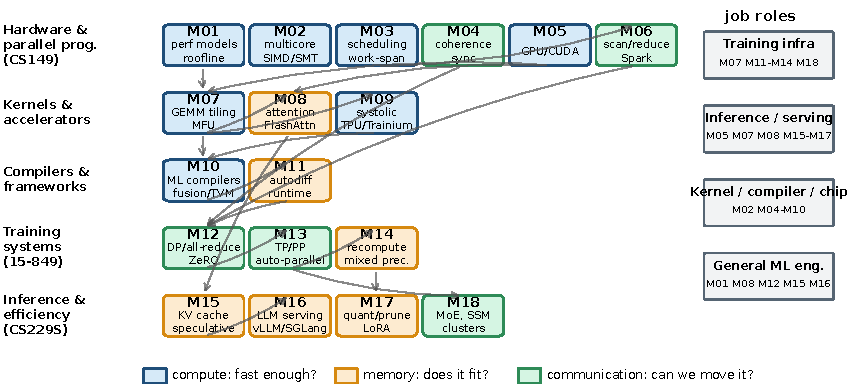
\includegraphics[width=\textwidth]{fig_capability_map}
\caption{18 个模块的知识地图。纵向按系统栈自下而上排列（硬件与并行编程 → 算子与加速器 → 编译器与框架 →
训练系统 → 推理与效率），颜色表示该模块主要回答的问题：蓝色「算得过来」、橙色「放得下」、绿色「传得过来」。
箭头是先修依赖，右侧是四类岗位的主线模块。面试准备时应沿箭头自下而上补齐，而不是按课程顺序线性阅读。}
\label{fig:map}
\end{figure*}

\subsection{三门课程如何互补}

三门课各管一层（表~\ref{tab:modules}）。CS149~\cite{cs149} 讲机器怎么并行：多核、SIMD、GPU、cache coherence、
内存一致性与专用硬件，给「算得过来」打地基。CS229S~\cite{cs229s} 把这些原理用在 Transformer 上：
hardware-aware 算法设计、FlashAttention、KV cache、推测解码、量化与新架构。CMU 15-849~\cite{cmu15849} 是论文研讨课，
覆盖框架、编译器、数据/模型/流水线并行、ZeRO、重计算与压缩，主要回答「放得下」和「传得过来」。
本文不按课程分章，而按系统栈自下而上排成 18 个模块，并补充了课程之后出现、但 2025 年以后推理岗默认要掌握的系统，
例如 vLLM~\cite{kwon2023vllm}、SGLang~\cite{zheng2024sglang}、FlashAttention-3~\cite{shah2024flashattention3}、
chunked prefill~\cite{agrawal2024sarathi} 与 PD 分离~\cite{zhong2024distserve,patel2024splitwise}。

\begin{table*}[!t]
\centering
\caption{18 个模块与三门课程、三个问题和配套实验的对应关系}
\label{tab:modules}
\footnotesize
\begin{tabularx}{\textwidth}{@{}c L{3.6cm} Y Y Y c L{2.6cm}@{}}
\toprule
\# & 模块 & CS149 Fall 2024 & CS229S Fall 2023 & CMU 15-849 S22 & 问题 & 本文配套实验 \\
\midrule
01 & 性能模型与 roofline & Why Parallelism & Hardware-aware algorithm design & Intro to DL systems & 算 & — \\
02 & 多核、SIMD 与多线程 & Multi-core, ISPC & — & — & 算 & CS149 A1 \\
03 & 并行编程与调度 & Work distribution, scheduling & — & — & 算 & CS149 A2 \\
04 & 局部性、一致性与同步 & Coherence, consistency, locks & — & — & 传 & CS149 A2 \\
05 & GPU 架构与 CUDA & GPU architecture, CUDA & GPU 存储层次 & — & 算 & CS149 A3 \\
06 & 数据并行原语 & Data-parallel thinking, Spark & — & Parameter server & 传 & CS149 A3 \\
07 & 矩阵乘与分块 & Efficiently evaluating DNNs & Hardware-aware design & ML hardware & 算 & CS149 A4 \\
08 & Attention 与 FlashAttention & DNN 融合 & FlashAttention & Transformers & 放 & CS229S P1 \\
09 & 专用加速器 & Hardware specialization & — & TPU & 算 & CS149 A4 \\
10 & ML 编译器 & Domain-specific prog. systems & TVM（客座） & ML compilation, TASO & 算 & 15-849 编译 \\
11 & 框架与自动微分 & — & FLOPs 与反传 & Systems for DL & 放 & 15-849 编译 \\
12 & 数据并行与 ZeRO & — & Parallelism fundamentals & Data parallel, ZeRO & 传 & 15-849 分布式 \\
13 & 张量/流水线并行 & — & Narayanan（客座） & Pipeline, Megatron, GSPMD & 传 & 15-849 分布式 \\
14 & 显存优化 & — & Dettmers（客座） & Rematerialization, Offload & 放 & 15-849 分布式 \\
15 & KV cache 与推测解码 & — & Analyzing Transformers & — & 放 & CS229S P2 \\
16 & LLM 推理服务 & — & Scheduling ML clusters & 推理库（客座） & 放 & 15-849 服务 \\
17 & 压缩、量化与 PEFT & — & Memory-efficient NN & Model compression & 放 & 15-849 编译 \\
18 & MoE、SSM、集群与数据 & — & Attention-free, MoE & GNN, ML for systems & 传 & — \\
\bottomrule
\end{tabularx}
\end{table*}

\subsection{本文的定位与贡献}

现有综述大多以「技术谱系」为线索，例如分布式训练综述或推理优化综述。本文的读者是准备 ML infra 面试、
或希望从工程走向研究的工程师，因此组织原则不同：每一个技术点都以「能否当场估算」和「能否说出常见错答」为验收标准。
具体贡献如下：
\begin{enumerate}
\item \textbf{统一的三问题框架}。把 18 个模块的内容组织到式~\eqref{eq:three} 的三项里，使读者能把陌生问题归约到熟悉的估算。
\item \textbf{可复算的数字}。正文中的每个数字要么在文中推导，要么由配套计算器 \texttt{tools/mlsys\_calc.py} 计算
（图表由 \texttt{reports/survey/make\_figures.py} 直接调用该计算器生成），要么引自论文或配套实验 CSV。
\item \textbf{配套实验与诚实的口径}。我们复用了仓库中 9 个 CPU 实验（FlashAttention IO 模型、KV cache 与推测解码、
分布式训练模拟、PagedAttention 服务模拟、编译/自动微分/压缩等）的结果，并逐条标明哪些是正确性验证、哪些是模型输出、
哪些是 CPU 实测，不能外推到 GPU。
\item \textbf{面试能力框架}。第~\ref{sec:interview} 节给出区分工程能力与研究能力的能力矩阵、答题模板、
常见错答清单、把实验转成 STAR 故事的方法以及研究能力练习。
\end{enumerate}

\begin{qa}{面试官为什么总让你「估一下」，而不是直接问概念？}
\ans 概念可以背，估算不行。估算同时检验三件事：是否知道硬件数量级（H100 约 1~PFLOP/s、3.35~TB/s），
是否会把系统行为化成公式（例如 decode 一步至少要读一遍权重），以及是否能从数字推出设计结论（例如 batch 不大时
量化比换卡更有效）。一个合格的回答在 30 秒内给出量级，再说明假设与误差来源。
\wrong 直接报一个经验数字（「大概 100~ms 吧」）而不给推导；或者花 5 分钟推导而不先报结论。
\end{qa}

\subsection{论文组织}

第~\ref{sec:perf} 节建立性能模型；第~\ref{sec:hw} 节讨论并行硬件与 GPU 编程模型；第~\ref{sec:kernel} 节讨论 GEMM、
FlashAttention 与融合；第~\ref{sec:accel} 节讨论专用加速器；第~\ref{sec:compiler} 节讨论编译器与框架；
第~\ref{sec:train} 节讨论分布式训练；第~\ref{sec:infer} 节讨论 LLM 推理与服务；第~\ref{sec:eff} 节讨论模型效率与架构；
第~\ref{sec:cluster} 节讨论集群、可靠性与数据；第~\ref{sec:interview} 节给出面试能力框架；
第~\ref{sec:open} 节讨论开放问题；附录给出公式速查、硬件参数与两周学习计划。
每节末尾有「面试要点」与「研究视角」两个框，前者用于考前复习，后者用于把知识变成可做的实验。

\section{性能模型：先算上界，再谈优化}
\label{sec:perf}

性能模型的价值不在于精确预测，而在于给出\emph{可被违反就说明有 bug 的上界}。本节介绍面试中最常用的五个模型：
roofline、Amdahl/Gustafson、work--span、Little 定律以及 I/O 复杂度下界。

\subsection{Roofline 与算术强度}

Williams 等人提出的 roofline 模型~\cite{williams2009roofline} 把一个 kernel 抽象为两个数：浮点运算量 $F$ 与
它在某一级存储（通常是 DRAM/HBM）上搬运的字节数 $B$。定义算术强度 $I=F/B$（FLOP/byte），则在计算与访存可重叠时
\begin{equation}
t \ge \max\!\left(\frac{F}{P_{\text{peak}}},\ \frac{B}{\mathrm{BW}}\right),\qquad
P_{\text{attain}} = \min(P_{\text{peak}},\ I\cdot \mathrm{BW}).
\label{eq:roofline}
\end{equation}
两项相等的点 $I^\ast = P_{\text{peak}}/\mathrm{BW}$ 称为拐点（ridge point）：$I<I^\ast$ 的 kernel 受访存限制（memory-bound），
$I>I^\ast$ 的受算力限制（compute-bound）。以本文统一使用的参数（附录表~\ref{tab:hw}）计算，H100 SXM 的稠密 BF16
峰值为 989~TFLOP/s、HBM3 带宽 3.35~TB/s，拐点 $I^\ast\approx 295$~FLOP/B；A100 SXM 为 312~TFLOP/s 与 2.04~TB/s，
$I^\ast\approx 153$~FLOP/B~\cite{nvidiaa100,nvidiah100}。注意 H100 的算力相对 A100 增加了 3.2 倍，带宽只增加了 1.6 倍，
所以拐点右移了近一倍：\emph{同一个 kernel 在新硬件上更容易变成访存受限}，这是「内存墙」~\cite{gholami2024memorywall}
在单卡上的体现。

图~\ref{fig:roofline} 把 Transformer 中几类典型算子放到 H100 的 roofline 上。逐元素加法（bf16，读两个、写一个元素，共 6 字节、1 FLOP）
强度只有 0.17，只能用到峰值的 0.06\%；LayerNorm/softmax 在 1 量级；batch=1 的 decode GEMV 强度约为 1；
GQA-8 的 decode attention 约为 4（第~\ref{sec:infer} 节推导）；batch=64 的 decode GEMM 约 62；$4096^3$ 的 prefill GEMM
达到 1365，远在拐点右侧。图中 FlashAttention 前向（点 7）与「S、P 各读写一次」的朴素实现（点 6）的强度差距不大，
这一点将在第~\ref{sec:kernel} 节由配套实验详细解释。

\begin{figure}[!t]
\centering
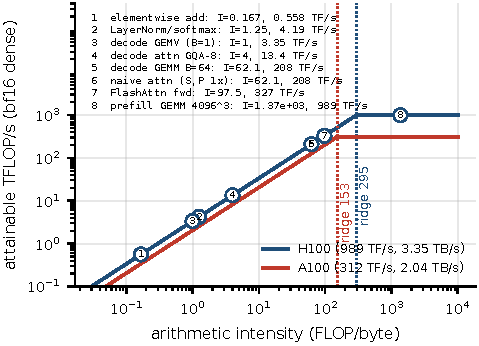
\includegraphics[width=\columnwidth]{fig_roofline}
\caption{A100 与 H100 的 roofline（BF16 稠密，HBM），以及 Transformer 典型算子在 H100 上的位置。
强度由 \texttt{mlsys\_calc.gemm\_intensity} 与配套 FlashAttention IO 模型（$T=4096,d=128$，SRAM 100~KiB）计算。
只有大 GEMM 越过拐点；decode 相关的全部算子位于斜线段，离拐点差 1--2 个数量级。}
\label{fig:roofline}
\end{figure}

roofline 的三个常见误用值得面试时主动指出。第一，$B$ 必须对应某一级存储；对 L2 或 shared memory 也可以画 roofline，
得到的拐点不同（层次化 roofline）。第二，$P_{\text{peak}}$ 必须对应实际使用的计算单元：A100 的非 tensor-core FP32 只有
19.5~TFLOP/s，与 BF16 tensor core 差 16 倍；FlashAttention-2 减少非矩阵乘 FLOPs 的动机正是这一点~\cite{dao2024flashattention2}。
第三，「GPU 利用率 100\%」不是算力打满：\texttt{nvidia-smi} 的 utilization 只表示采样窗口内有 kernel 在运行。

\begin{qa}{为什么「GPU 利用率 100\%」不代表算力打满？应该看什么？}
\ans \texttt{nvidia-smi} 报告的是有 kernel 驻留的时间比例，一个访存受限的逐元素 kernel 同样可以显示 100\%。
应看 Nsight Compute 的 SM 吞吐与 DRAM 吞吐占峰值的比例，或者直接计算 MFU（模型 FLOPs 利用率，第~\ref{sec:kernel} 节）。
DRAM 吞吐接近峰值而 SM 吞吐低，说明受访存限制，下一步是融合或降低精度，而不是调 block size。
\wrong 「100\% 说明已经最优」；或把 HFU（含重计算 FLOPs）当成 MFU 报告。
\end{qa}

\subsection{Amdahl 与 Gustafson 定律}

设程序中可并行部分占比为 $p$，用 $n$ 个处理器时，Amdahl 定律~\cite{amdahl1967validity} 给出固定问题规模下的加速比
\begin{equation}
S_{\text{A}}(n) = \frac{1}{(1-p) + p/n} \xrightarrow{n\to\infty} \frac{1}{1-p}.
\end{equation}
Gustafson~\cite{gustafson1988reevaluating} 指出，实际中问题规模常随资源增长，若并行部分的工作量放大 $n$ 倍，
则 $S_{\text{G}}(n)=(1-p)+pn$。图~\ref{fig:amdahl} 对比了两者：$p=0.95$ 时 8 核只有 5.9 倍，无穷多核也只有 20 倍；
而 Gustafson 视角下加速比随 $n$ 近似线性增长。两者并不矛盾：前者回答「同一个任务能快多少」，
后者回答「同样的时间能做多大的任务」。大模型训练中的弱扩展（增大 global batch）正是 Gustafson 视角，
但它受临界 batch size 的限制，不能无限扩展。

\begin{figure}[!t]
\centering
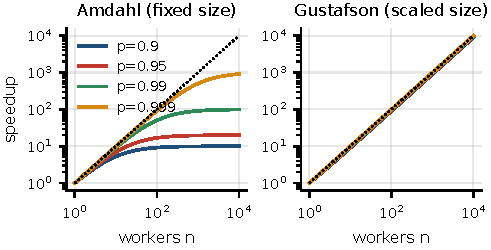
\includegraphics[width=\columnwidth]{fig_amdahl}
\caption{Amdahl（固定规模）与 Gustafson（规模随处理器数增长）加速比，虚线为线性加速。
$p=0.99$ 时 1024 个处理器的 Amdahl 加速比只有 91 倍（\texttt{mlsys\_calc.amdahl\_speedup}）。}
\label{fig:amdahl}
\end{figure}

\begin{qa}{Amdahl 定律在大模型训练里体现在哪里？}
\ans 体现在不随卡数缩小的部分：dataloader 的串行段、优化器步进中的全局梯度范数、日志与 checkpoint、
all-reduce 的延迟项 $2(p-1)\alpha$、流水线气泡，以及负载不均时最慢的 rank。卡数上去之后，这些部分决定 MFU 的上限。
\wrong 「训练是完全数据并行的，没有串行部分」。
\end{qa}

\subsection{Work--span 模型与调度}

把并行计算建模为有向无环图，$T_1$ 为总工作量（work），$T_\infty$ 为关键路径长度（span），并行度为 $T_1/T_\infty$。
Brent 定理~\cite{brent1974parallel} 与贪心调度给出
\begin{equation}
T_P \le \frac{T_1}{P} + T_\infty,
\label{eq:brent}
\end{equation}
Blumofe 与 Leiserson 证明随机 work stealing 在期望意义下达到 $T_1/P+O(T_\infty)$~\cite{blumofe1999scheduling}：
每个线程从自己的双端队列尾部取任务，空闲时随机从别人队列头部「偷」，偷到的往往是大块工作，争抢少。
式~\eqref{eq:brent} 的直接推论是线性加速的条件 $P\ll T_1/T_\infty$。

scan（前缀和）是检验 work--span 思维的标准例子~\cite{blelloch1990prefix,hillis1986data}。Hillis--Steele 算法 span 为 $\log_2 n$，
work 为 $n\log_2 n$；Blelloch 算法 work 为 $2(n-1)$，span 为 $2\log_2 n$。
\lab{CS149 A3}的计数器与公式逐一相等：$n=2^{20}$ 时 Blelloch 做 2.10M 次加法、40 步，Hillis--Steele 做 19.9M 次、20 步；
处理器多于数据时（$n=1000,P=2048$）Hillis--Steele 的 Brent 上界 15 低于 Blelloch 的 21，处理器少时 work 主导，Blelloch 胜出。
GPU 上的工程结论是：大数组用 work-efficient 的 Blelloch，warp 内（32 个元素）用 Hillis--Steele，因为线程本来就空着。

负载均衡是 work--span 的另一面。\lab{CS149 A1}在 Mandelbrot 上比较了三种划分：4 个 worker 时连续块划分 2.93 倍、
交错行 3.93 倍、动态分块 3.76 倍；8 块静态划分时中间块耗时 0.233~s 而边缘块只有 0.063~s。
同一实验的第一版曾测出 8 个 worker 21 倍的「超线性加速」，原因是按 worker 数切块改变了 numpy 中间数组的缓存行为，
基线不公平——这是一个很好的面试故事：超线性加速首先怀疑基线。

\begin{qa}{静态分配和动态分配怎么选？work stealing 为什么好？}
\ans 任务代价可预测且均匀时用静态划分（零调度开销）；不可预测时用动态。集中式队列会成为争抢热点，work stealing 让每个线程
优先处理本地任务，只有空闲时才偷，并且偷队列另一端的大块任务，满足 $T_P\le T_1/P+O(T_\infty)$。
\wrong 「动态一定比静态好」——细粒度任务的入队出队开销可能比任务本身还大。
\end{qa}

\subsection{Little 定律与服务容量}

对任何稳态排队系统，Little 定律~\cite{little1961proof} 给出 $L=\lambda W$：系统中平均请求数等于到达率乘以平均停留时间。
它不依赖到达分布与服务分布，因此是推理服务容量规划的第一公式。设平均输出 500 token、每 token 时延（TPOT）30~ms、
首 token 时延（TTFT）0.5~s，则 $W\approx 15.5$~s；若 KV 预算只允许 64 条并发，则 $\lambda_{\max}\approx 64/15.5\approx 4.1$~req/s。
同样的定律也解释了 GPU 的延迟隐藏：要维持带宽 $\mathrm{BW}$、访存延迟 $\ell$，在途字节数必须达到 $\mathrm{BW}\cdot\ell$，
这是 occupancy 与异步拷贝存在的理由（第~\ref{sec:hw} 节）。

\begin{est}{H100 需要多少在途字节才能吃满 HBM？}
取 HBM 带宽 3.35~TB/s、访存延迟约 500 个周期（约 0.3~\textmu s，附录表~\ref{tab:hw} 的数量级）。
由 Little 定律，在途字节 $\approx 3.35\times10^{12}\times 3\times10^{-7}\approx 1$~MB；分到 132 个 SM，每个 SM 约 7.6~KB 在途。
若每个线程每次发起 16 字节的向量加载，每个 SM 需要约 480 个线程同时有访存在途。这就是为什么访存受限 kernel
需要较高 occupancy 或者 TMA/\texttt{cp.async} 这类异步批量拷贝。
\end{est}

\subsection{I/O 复杂度下界}

Hong 与 Kung 的红蓝卵石游戏~\cite{hong1981io} 证明，快速存储容量为 $M$ 时，$n\times n$ 矩阵乘至少需要
$\Omega(n^3/\sqrt{M})$ 次慢速存储访问。这个下界把「分块」从技巧变成了必然：任何达到下界的算法都必须让每个
加载进快存的元素被复用 $\Theta(\sqrt{M})$ 次。FlashAttention 论文给出了 attention 的类似下界
$\Omega(T^2d^2/M)$~\cite{dao2022flashattention}，我们在第~\ref{sec:kernel} 节会看到，这个下界在 $d^2/M$ 不太小时
意味着 HBM 流量仍是 $T$ 的二次函数。

\begin{keypts}
\begin{itemize}
\item roofline：$t\ge\max(F/P,B/\mathrm{BW})$；H100 拐点 295、A100 拐点 153~FLOP/B，必须说明对应哪个计算单元与哪级存储。
\item Amdahl 给固定规模的上限，Gustafson 给扩展规模的视角；训练中的串行项包括通信延迟与流水线气泡。
\item work--span：$T_P\le T_1/P+T_\infty$；scan 的两种算法分别优化 span 与 work。
\item Little 定律 $L=\lambda W$ 同时适用于服务容量和 GPU 延迟隐藏。
\end{itemize}
\end{keypts}

\begin{research}
\begin{itemize}
\item roofline 假设计算与访存完全重叠。一个好问题是：对于 FlashAttention 这类「矩阵乘 + 逐元素」交替的 kernel，
重叠不完美导致的偏差有多大？可以用 Nsight 的指令级采样把时间分解为 tensor core 忙、等待 TMA、等待 softmax 三部分。
\item 设计实验验证 Little 定律在 LLM 服务里的适用边界：在 continuous batching 下，停留时间 $W$ 本身依赖并发 $L$
（batch 越大每步越慢），系统是否仍存在唯一稳态？
\end{itemize}
\end{research}

\section{并行硬件与编程模型}
\label{sec:hw}

本节对应 CS149 的前半部分。我们沿着「如何把晶体管变成吞吐」这条线，依次讨论多核、SIMD、硬件多线程、
cache coherence 与内存一致性，再把这些概念映射到 GPU 的 SIMT 模型上。面试中这一层的问题看似基础，
但它们是回答「为什么这个 kernel 慢」的唯一依据。

\subsection{多核、SIMD 与硬件多线程}

现代处理器用三种正交的手段提高吞吐~\cite{hennessy2019golden}：（1）\textbf{多核}，复制整个取指--执行流水线；
（2）\textbf{SIMD}，一条指令驱动 $W$ 个 ALU（AVX2 为 8 个 fp32 lane，AVX-512 为 16 个），把取指译码开销摊到 $W$ 个数据上；
（3）\textbf{硬件多线程}（SMT），在一个核上保存多个线程的上下文，一个线程等待内存时切换到另一个线程。
三者分别利用了任务并行、数据并行与延迟隐藏。GPU 把三者推到极致：H100 有 132 个 SM，每个 SM 同时驻留最多 64 个 warp，
每个 warp 32 个线程以 SIMT 方式执行~\cite{lindholm2008tesla,nickolls2008cuda}。

\textbf{SIMD 发散}（divergence）是数据并行的主要效率损失。一组 $W$ 个 lane 必须执行到组内最慢的 lane 结束，因此利用率为
\begin{equation}
U = \frac{\sum_{i} w_i}{W\cdot \max_{i\in\text{gang}} w_i},
\end{equation}
其中 $w_i$ 为第 $i$ 个 lane 的有效迭代数。\lab{CS149 A1}的模拟显示，每个 8 宽 gang 中只要有一条慢 lane，
利用率就跌到 0.163（加速 1.30 倍而非 8 倍）；在 numpy 中实测，掩码执行在「每 16 个元素有 1 个慢元素」的输入上与全部都慢的输入
一样贵（353 对 356~ns/元素），先压缩活跃集合后降到 29~ns。GPU 的 warp 发散与此完全同构，工程解法是按工作量排序或分桶，
让同一个 warp 内线程的工作量接近，或者改为持续从队列拉取工作的 persistent kernel。

\begin{qa}{SIMD/warp 发散的代价怎么算？if/else 只执行一个分支，为什么还有代价？}
\ans 同一 warp 的线程共享一个程序计数器（Volta 之后有独立线程调度，但发散路径仍串行化），两个分支依次执行，
不活跃的 lane 被掩码。代价为 $W\cdot\max w_i/\sum w_i$ 倍。工作量差异越大，代价越高。
\wrong 「if/else 两个分支只执行一个，所以没有代价」；或者认为发散只发生在 GPU 而不发生在 CPU SIMD 上。
\end{qa}

\textbf{硬件多线程}用并发换延迟：若访存延迟为 $\ell$ 周期、每个线程两次访存之间平均有 $c$ 个周期的计算，
则约需 $\ell/c$ 个线程才能让核保持忙碌。代价是每个线程都要占用寄存器与上下文，片上存储被分摊。
GPU 的 occupancy（每个 SM 驻留 warp 数与上限之比）就是这件事的量化。

\subsection{Cache coherence、false sharing 与同步}

多核共享内存时，每个核私有的 cache 需要一致性协议。MESI 一类基于失效的协议~\cite{papamarcos1984low} 保证单个地址上
「写串行化」：一个核写某 cache line 前必须使其它核的副本失效。由此产生了 \textbf{false sharing}：
两个核写同一 64 字节 cache line 上的不同变量，协议让这条 line 在两个核之间来回迁移（每次数十到上百 ns），
表现为加线程反而变慢。修法是按 cache line 填充或让每个线程写私有副本，最后归约。

一致性（coherence）只约束单个地址；\textbf{内存一致性模型}（consistency）约束不同地址之间读写的可见顺序。
顺序一致性（SC）~\cite{lamport1979make} 要求所有核看到同一个全局交错顺序；x86 的 TSO 允许「写后读」重排（store buffer），
ARM 与 GPU 采用更弱的模型~\cite{adve1996shared}。程序员通过 fence 或 acquire/release 原子操作建立
happens-before 关系。GPU 上的典型陷阱是：用一个普通标志位在 block 之间传递「数据已就绪」，没有 \texttt{\_\_threadfence()}
时另一个 SM 可能先看到标志后看到数据。

无锁数据结构依赖 CAS（compare-and-swap），其经典问题是 \textbf{ABA}：线程读到栈顶 A 后被挂起，其他线程弹出 A、弹出 B、
再压回 A，CAS 仍然成功，但 A 的 next 指针已失效。解法是带版本号的指针、hazard pointer 或 epoch 回收。

\begin{qa}{什么是 false sharing？怎么发现，怎么修？}
\ans 不同核写同一 cache line 上的不同变量，coherence 协议使该 line 反复失效迁移。症状是线程数增加而吞吐下降，
perf 中 HITM（命中其它核修改过的 line）事件很高。修法：按 64~B 对齐填充每线程计数器，或写线程私有副本再归约。
\wrong 「没有共享变量就没有竞争」——竞争的单位是 cache line，不是变量。
\end{qa}

\begin{qa}{x86 上一个线程写 \texttt{data=1; flag=1}，另一个线程 \texttt{while(!flag); print(data)}，一定打印 1 吗？在 ARM 或 GPU 上呢？}
\ans x86 的 TSO 不重排「写--写」与「读--读」，所以硬件层面会打印 1，但编译器仍可能重排或把 \texttt{flag} 提到寄存器里，
必须用 \texttt{std::atomic} 的 release/acquire。ARM 与 GPU 的弱内存模型允许写--写重排，没有 fence 时可能打印 0。
\wrong 「有 cache coherence 就一定看到最新值」——coherence 不约束不同地址之间的顺序。
\end{qa}

同步原语的选择是另一个高频题。\lab{CS149 A2}在 Python 中复刻了 CS149 的任务系统，测得 8 个空任务一次 launch：
条件变量（sleep）线程池 38.7~\textmu s，每次新建线程 3169~\textmu s，纯自旋线程池 31--50~ms。后者在 C++ 中本应最快，
但在 CPython 中自旋线程持有 GIL，要等 5~ms 的切换间隔才让出，空闲时还烧满 1 个核。这个实验的价值在于说明
\emph{「spin 还是 sleep」取决于自旋者是否阻塞干活的线程}，而不是一个与平台无关的定论。
同一实验中，异步依赖图让 48 个 9 任务的 launch 从 259~ms 降到 152~ms，接近理想比值 $2/(9/8)=1.78$
（实测 1.71 倍），这是「填满尾部空闲」的直接证据，与 CUDA stream 和 CUDA Graph 的动机相同。

\subsection{GPU 的 SIMT 编程模型}

CUDA 把计算组织为 grid--block--thread 三级，block 内的线程可以通过 shared memory 通信并用 \texttt{\_\_syncthreads()} 同步，
block 之间默认独立~\cite{nickolls2008cuda}。硬件上 block 被调度到 SM，SM 以 32 线程的 warp 为单位发射指令。
H100 的存储层次见表~\ref{tab:gpumem}：寄存器与 shared memory 的带宽比 HBM 高一个数量级以上，延迟低一个数量级，
所以几乎所有 GPU 优化都是把数据「搬近、复用、搬远」三步~\cite{volkov2010better,cutlass}。

\begin{table}[!t]
\centering
\caption{H100 SXM 存储层次的数量级（附录表~\ref{tab:hw} 的子集）}
\label{tab:gpumem}
\footnotesize
\begin{tabularx}{\columnwidth}{@{}l l l Y@{}}
\toprule
层级 & 容量 & 带宽量级 & 延迟与说明 \\
\midrule
寄存器 & 256~KB/SM & — & 1 周期；寄存器分块是 GEMM 复用的最内层 \\
Shared/L1 & $\le$228~KB/SM & $\sim$30~TB/s（全卡） & 20--30 周期；软件管理，32 个 bank \\
L2 & 50~MB & $\sim$10~TB/s & $\sim$200 周期；K/V 重读多命中于此 \\
HBM3 & 80~GB & 3.35~TB/s & $\sim$500 周期；roofline 的默认 $B$ \\
主机内存 & 数百 GB & 32--64~GB/s & 微秒级；经 PCIe，offload 的瓶颈 \\
\bottomrule
\end{tabularx}
\end{table}

\textbf{访存合并}（coalescing）：一个 warp 的 32 个线程访问连续且对齐的地址时，硬件合并为少量 32~B/128~B 事务；
按列访问行主序矩阵（stride 等于行宽）时每个线程一个事务，有效带宽下降一个数量级。常用的修法是借 shared memory 做转置中转。

\textbf{Bank conflict}：shared memory 分为 32 个 bank、每 bank 4 字节宽。同一 warp 的线程访问同一 bank 的不同地址会被串行化。
典型例子是 $32\times32$ 的 float 矩阵按列读取，所有线程落在同一 bank；声明为 $32\times33$（填充一列）即可错开。
同一地址的广播不冲突。

\begin{qa}{什么是 memory coalescing？给一个不合并的例子。}
\ans 合并的单位是 warp，看的是 32 个线程地址的模式：连续对齐时一个 128~B 事务就能服务整个 warp。
行主序矩阵按列读、结构体数组（AoS）只读一个字段、随机 gather 都不合并。修法：改数据布局（SoA）、shared memory 转置、
或者让相邻线程处理相邻元素。
\wrong 「同一个 block 内的访问会自动合并」；或把 coalescing 与 shared memory bank conflict 混为一谈。
\end{qa}

\begin{qa}{Shared memory bank conflict 怎么产生、怎么避免？}
\ans 同一 warp 中多个线程访问同一 bank 的\emph{不同}地址时串行化。按列访问 $32\times32$ float 矩阵是 32 路冲突；
填充为 $32\times33$ 使第 $i$ 行第 $j$ 列落在 bank $(33i+j)\bmod 32$，冲突消失。Hopper 的 TMA 与 swizzle 布局也是为了这件事。
\wrong 「bank conflict 发生在 global memory」；「所有线程读同一地址也冲突」（那是广播）。
\end{qa}

\textbf{Occupancy} 是延迟隐藏的手段而不是目标。Volkov 的经典报告~\cite{volkov2010better} 指出，
依靠指令级并行（ILP）和寄存器分块，低 occupancy 的 kernel 可以更快：高性能 GEMM 常让每个线程计算 $8\times8$ 以上的输出块，
占用大量寄存器，occupancy 只有 25\% 左右，但数据复用显著更高。CUTLASS~\cite{cutlass} 的层次化分块
（threadblock tile → warp tile → MMA tile）把这一思想系统化。

\begin{qa}{occupancy 越高越好吗？}
\ans 不是。occupancy 只是隐藏延迟的一种方式，另一种是 ILP 与异步拷贝。寄存器分块很重的 GEMM 和 FlashAttention
故意降低 occupancy 换取复用。判断标准是吞吐：Nsight Compute 显示 stall 原因主要是「等待内存」时提高 occupancy 有用，
主要是「等待 tensor core」时没用。
\wrong 「把 occupancy 拉到 100\% 性能就最好」。
\end{qa}

\subsection{Tensor core 与 Hopper 的异步执行}

Volta 引入 tensor core，每个时钟完成一个小矩阵乘加~\cite{nvidiavolta2017}；Ampere 增加 BF16/TF32 与 2:4 结构化稀疏~\cite{nvidiaa100,mishra2021accelerating}；
Hopper 增加 FP8、TMA（Tensor Memory Accelerator，异步批量搬运张量块）、warpgroup 级的异步 MMA 指令（wgmma）
以及 thread block cluster 与分布式 shared memory~\cite{nvidiah100}。这些特性的共同方向是：
\emph{把搬运与计算交给不同的硬件单元异步执行}，让软件流水线（producer 负责搬运、consumer 负责计算）成为可能。
FlashAttention-3 的 warp specialization 正是建立在这些特性之上~\cite{shah2024flashattention3}。

\begin{keypts}
\begin{itemize}
\item 三种并行：多核（任务）、SIMD/SIMT（数据）、多线程（延迟隐藏）；发散的代价按组内最慢 lane 计。
\item coherence 管单地址，consistency 管多地址顺序；false sharing 的单位是 cache line；无锁结构注意 ABA。
\item GPU 三件事：合并访存（warp 地址模式）、bank conflict（shared memory）、occupancy（手段不是目标）。
\item Hopper 的方向是异步：TMA 负责搬、wgmma 负责算，软件用 warp specialization 把两者流水起来。
\end{itemize}
\end{keypts}

\begin{research}
\begin{itemize}
\item 如何自动选择 warp specialization 的 producer/consumer 划分与流水深度？这是一个带资源约束（寄存器、shared memory）的
调度问题，目前多由专家手写（CUTLASS、FlashAttention-3）。
\item 设计一个微基准，测量 H100 上 shared memory bank conflict、L2 命中与 TMA 异步拷贝对一个 tile 化 GEMM 的各自贡献；
关键是每次只改变一个因素，并给出与 roofline 上界的差距分解。
\end{itemize}
\end{research}

\section{算子与内核：GEMM、FlashAttention 与融合}
\label{sec:kernel}

Transformer 的 FLOPs 绝大部分在 GEMM 里，而端到端时间的相当一部分却花在访存受限的「小算子」和 attention 的中间矩阵上。
本节先推导 GEMM 分块的复用与上界，再详细讨论 FlashAttention 三个版本以及一个经常被误解的问题——
它到底把 HBM 流量降了多少，最后讨论融合与 Triton。

\subsection{GEMM 的算术强度与分块}

$C_{M\times N}=A_{M\times K}B_{K\times N}$ 的运算量为 $F=2MNK$（一次乘加记 2 FLOP，厂商峰值也按此计）。若三个矩阵各过一次 HBM，
\begin{equation}
\begin{gathered}
I_{\text{GEMM}} = \frac{2MNK}{s(MK+KN+MN)},\\
I_{\text{square}} = \frac{2n}{3s},\qquad
I_{\text{GEMV}} \approx \frac{2}{s},
\end{gathered}
\end{equation}
其中 $s$ 为每元素字节数。BF16 方阵的强度为 $n/3$，在 H100 上要 $n\gtrsim 900$ 才越过拐点 295；
GEMV（$M=1$）只有 1~FLOP/B，只能用到峰值的 1/295。这一个式子解释了 decode 为什么慢、为什么 batch 是推理吞吐的第一杠杆。

上式假设「每个矩阵只过一次 HBM」，这要求片上能放下足够大的块。设快存可放 $M_s$ 个元素，采用 $b\times b$ 方块且三块同时驻留，
则 $3b^2\le M_s$。每加载两个 $b\times b$ 块做 $2b^3$ 次运算，局部强度约为 $b/s$；总访存
\begin{equation}
Q \approx \frac{2n^3}{b}+n^2 = \Theta\!\left(\frac{n^3}{\sqrt{M_s}}\right),
\end{equation}
与 Hong--Kung 下界同阶~\cite{hong1981io}。

\begin{est}{H100 一个 SM 的 shared memory 能支撑多大的 GEMM 块？}
H100 每 SM 最多 228~KB shared memory。BF16 下 $3b^2\times2\le228$~KB 得 $b\le197$，工程上取 128。此时单个 block 的局部强度
$b/s=64$~FLOP/B，\emph{还不到}拐点 295。真实 kernel 靠三件事越过拐点：多个 thread block 在 50~MB 的 L2 中共享 A、B 的同一行块/列块
（L2 带宽约为 HBM 的 3 倍）；非方形块（如 $128\times256$）；以及寄存器层再分块。这说明面试中「块越大越好」的回答不完整：
块大小受 shared memory、寄存器、occupancy 与 SM 数量（块数要足以填满 132 个 SM）的共同约束。
\end{est}

\lab{CS149 A4}在一个带 SBUF/PSUM 容量约束的 Trainium 式分块模型上验证了同样的规律：$4096^3$ 的 BF16 GEMM，
tile 边长从 128 增至 256、512 时 HBM 强度为 63.0、124.1、240.9~FLOP/B，约等于边长的一半；SBUF $\ge$1~MiB 之后，
2~MiB 的 PSUM（FP32 累加器）把强度封顶在 315.1；再增大 SBUF 只能加大 $t_k$、把 DMA 次数从 2080 降到 96，不再提高强度。
这些加速器参数是模型假设，不能当成 Trainium 规格（第~\ref{sec:accel} 节）。

\begin{qa}{矩阵乘分块时块大小怎么选？}
\ans 四个约束：（1）容量：$3b^2 s\le M_s$（双缓冲时再减半）；（2）强度：局部强度约 $b/s$，需结合 L2 复用越过拐点；
（3）并行度：$(M/b_m)(N/b_n)$ 个块要足以填满所有 SM，小矩阵常用 split-K；（4）硬件形状：块要是 MMA 指令形状的整数倍，
并兼顾 occupancy 与寄存器压力。最终由 autotuning 在候选集合中选。
\wrong 「越大越好」；或只考虑 shared memory 容量而忽略 SM 数与波次（wave quantization）。
\end{qa}

\textbf{MFU}（model FLOPs utilization）是训练效率的标准口径~\cite{chowdhery2022palm}：
$\mathrm{MFU}=6N\cdot(\text{tokens/s})/(n_{\text{GPU}}P_{\text{peak}})$。例如 8 张 H100 训练 7B 模型达到每秒 $10^5$ token，
MFU $=6\times7\times10^9\times10^5/(8\times989\times10^{12})\approx 53\%$。HFU 把重计算的 FLOPs 也算进去，所以 $\mathrm{HFU}\ge\mathrm{MFU}$。
MegaScale 报告在 12,288 张 GPU 上训练 175B 模型达到 55.2\% MFU~\cite{jiang2024megascale}，可作为大规模训练 MFU 的参考量级。

\begin{qa}{batch=1 的矩阵--向量乘为什么在任何 GPU 上都慢？}
\ans BF16 GEMV 的强度约为 1~FLOP/B，H100 拐点 295，只能用到峰值的 0.3\%。提高强度只有两条路：增加 batch（GEMV 变 GEMM），
或减少每个权重的字节数（量化）。换更快的卡帮助有限：H100 相对 A100 带宽只多 1.6 倍。
\wrong 「decode 慢是因为计算量大」。
\end{qa}

\subsection{Attention 的代价}

单头 attention 中 $Q,K,V\in\mathbb{R}^{T\times d}$，$S=QK^\top$ 与 $O=PV$ 各需 $2T^2d$ FLOPs，多头合计每层前向
$4T^2d_{\text{model}}$；朴素实现要物化 $T\times T$ 的 $S$ 与 $P$，每层每样本显存 $h\,T^2 s$ 字节。

\begin{est}{8K 上下文的 attention 占多少计算和显存？}
$T=8192$、$d_{\text{model}}=4096$、32 头、BF16：attention 前向 $4T^2d_{\text{model}}=4\times8192^2\times4096\approx1.1$~TFLOP/层；
同层投影与 MLP 约 $24Td_{\text{model}}^2\approx3.3$~TFLOP（按 4 倍 MLP 估），attention 约占 1/4。分数矩阵 $32\times8192^2\times2$~B
$\approx4.3$~GB/层/样本，反传还要保存。结论：中等长度下 attention 的问题首先是\emph{显存与 IO}，其次才是 FLOPs；
这正是 FlashAttention 的出发点。
\end{est}

\subsection{Online softmax 与 FlashAttention}

softmax 看似需要整行的最大值与和。Milakov 与 Gimelshein 的 online normalizer~\cite{milakov2018online} 观察到
$e^{x-m_{\text{new}}}=e^{x-m_{\text{old}}}\cdot e^{m_{\text{old}}-m_{\text{new}}}$，于是两段的统计量 $(m_i,\ell_i,o_i)$ 可以合并：
\begin{equation}
\begin{aligned}
m &= \max(m_1,m_2),\quad
\ell = e^{m_1-m}\ell_1 + e^{m_2-m}\ell_2,\\
o &= e^{m_1-m}o_1 + e^{m_2-m}o_2,\qquad O=o/\ell .
\end{aligned}
\label{eq:online}
\end{equation}
Rabe 与 Staats 据此证明 self-attention 只需 $O(\sqrt{n})$ 乃至 $O(\log n)$ 的额外显存~\cite{rabe2021selfattention}；
FlashAttention~\cite{dao2022flashattention} 把它与 GPU 存储层次结合：把 $Q$ 切成 $B_r$ 行一块、$K,V$ 切成 $B_c$ 行一块，
$S$、$P$ 的块只在 SRAM 中存在，反向传播保存每行的 logsumexp $L_i=m_i+\log\ell_i$，按块重算 $P_{ij}=\exp(S_{ij}-L_i)$。
它是\emph{精确}算法，不减少 FLOPs（反向还多一次 $QK^\top$ 重算），省的是 HBM 读写与显存：额外显存从 $O(T^2)$ 降到 $O(T)$。

\textbf{IO 复杂度}。SRAM 可放 $M$ 个元素，要同时放下 $K_j,V_j$ 与 $Q_i,O_i$，论文取 $B_c=\lceil M/4d\rceil$、
$B_r=\min(\lceil M/4d\rceil,d)$。外层每遍历一个 $K/V$ 块就要扫一遍全部 $Q,O$，总访问量
\begin{equation}
Q_{\text{flash}} = \Theta\!\left(\frac{T^2d^2}{M}\right),
\end{equation}
并且论文证明没有精确算法能在全部 $M\in[d,Td]$ 上做到 $o(T^2d^2/M)$~\cite{dao2022flashattention}。
关键在于：$d=64$--128、$M\approx10^5$ 时 $d^2/M$ 是一个常数（约 0.04--0.16），\emph{流量在 $T$ 上仍是二次的}，只是常数比朴素实现小。

\begin{figure*}[!t]
\centering
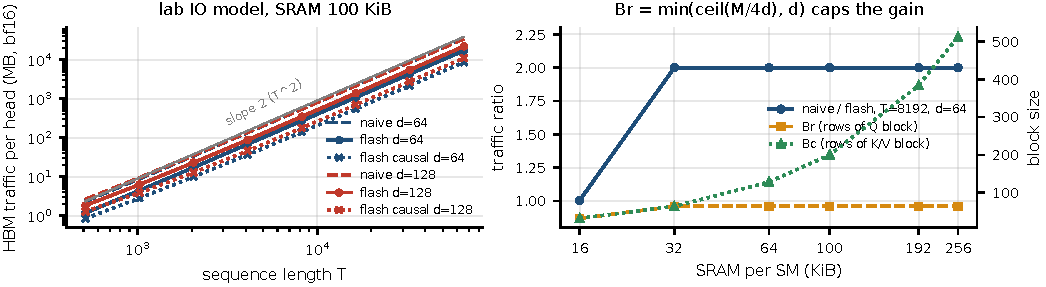
\includegraphics[width=\textwidth]{fig_lab_flash}
\caption{本文配套实验（CS229S P1）的 FlashAttention IO 计数器结果。左：每头 HBM 流量随 $T$ 的变化（BF16，SRAM 100~KiB），
朴素实现只计 $S$、$P$ 各读写一次；所有曲线斜率均为 2，即 $\Theta(T^2)$。非因果时 Flash 只比朴素少 2.00 倍（$d=64$）或 1.56 倍（$d=128$），
因果时由于跳过上三角块约少 4 倍。右：$T=8192,d=64$ 时流量比随 SRAM 的变化。$B_r$ 在 32~KiB 处即被 $d$ 截住，
更大的 SRAM 只增大 $B_c$，不再减少 $K/V$ 的重读次数。IO 计数器与解析模型在 8 组配置上逐元素一致。}
\label{fig:labflash}
\end{figure*}

图~\ref{fig:labflash} 是这一结论的直接证据。配套实验用 numpy 实现了 FA2 顺序的分块前向与基于 logsumexp 的反向，
float64 下 $O$、$dQ$、$dK$、$dV$ 与 \texttt{torch} 自动微分的最大误差 $\le4.9\times10^{-15}$；IO 计数器记录每次块读写。
$d=64$、$T=65536$ 时朴素 34,393~MB、Flash 17,197~MB，比值 2.00；$d=128$ 时 1.56。这与白板公式吻合：
Flash 流量 $\approx 2Td\cdot(T/B_r)+4Td$，朴素 $\approx4T^2$，比值 $\approx 2B_r/d$，$B_r=d$ 时为 2。
\emph{不能}由此推出「FlashAttention 在 GPU 上只快 2 倍」：真实 eager 实现中 scale、mask、softmax、dropout 各自对 $T^2$ 张量读写一次，
$S$ 常以 FP32 存储，且 $K/V$ 的重读在 GPU 上大多命中 L2；FlashAttention 最确定的收益是显存从 $O(T^2)$ 到 $O(T)$
以及消除这些中间 kernel。同样，numpy 版 Flash 比朴素版更慢（$T=1024,d=128$ 时 44.6 对 22.9~ms），这是 Python 循环开销，与 GPU 无关。

\begin{qa}{FlashAttention 快在哪？它减少了 FLOPs 吗？HBM 访问降到线性了吗？}
\ans 没有减少 FLOPs，反向还多一次重算；它是精确算法。快在不把 $T\times T$ 的分数矩阵写回 HBM：分块计算，用 online softmax 维护每行最大值与分母，
把 matmul--softmax--matmul 融合成一个 kernel。显存从 $O(T^2)$ 降到 $O(T)$；HBM 访问是 $\Theta(T^2d^2/M)$，对常见 $d$ 在 $T$ 上仍是二次，
只是常数显著变小。
\wrong 「它是近似 attention」；「访存从二次降到线性」——只有显存是线性的。
\end{qa}

\textbf{FlashAttention-2}~\cite{dao2024flashattention2} 的改动全部是工程性的（表~\ref{tab:fa}）：外层循环改为遍历 $Q$ 块，
每个 thread block 负责一段 $Q$，输出累加器留在寄存器、最后只写一次；推迟 rescale，只存 logsumexp，减少非矩阵乘 FLOPs
（A100 上非 tensor-core FLOP/s 比 tensor core 低约 16 倍）；除 batch 与 head 外还沿序列长度并行，长序列小 batch 时也能填满 SM；
block 内把 $Q$ 切给 4 个 warp，避免 v1 中 warp 间经 shared memory 归约。论文报告在 A100 上达到理论峰值的 50--73\%。

\textbf{FlashAttention-3}~\cite{shah2024flashattention3} 面向 Hopper：producer warp 只发 TMA 加载，consumer warpgroup 做 wgmma 与 softmax
（warp specialization）；两个 consumer warpgroup ping-pong，使一个做 softmax 时另一个做 GEMM；同一 warpgroup 内也让 softmax 与下一块 GEMM 重叠；
FP8 路径用分块量化与 Hadamard 变换（incoherent processing）压低离群值误差。论文报告 H100 上 BF16 约 740~TFLOP/s（约 75\% 利用率）。

\begin{table}[!t]
\centering
\caption{FlashAttention 三个版本的对比}
\label{tab:fa}
\footnotesize
\begin{tabularx}{\columnwidth}{@{}l Y Y Y@{}}
\toprule
 & FA1 (2022) & FA2 (2023) & FA3 (2024) \\
\midrule
目标硬件 & A100 等 & A100 & H100 (Hopper) \\
外层循环 & $K/V$ 块 & $Q$ 块 & $Q$ 块 \\
$O$ 的写回 & 每个 $K/V$ 块读写一次 & 只写一次 & 只写一次 \\
并行维度 & batch$\times$head & + 序列长度 & + warp specialization \\
warp 分工 & 按 $K/V$ 切，需归约 & 按 $Q$ 切，无归约 & producer\slash consumer、ping-pong \\
非 matmul FLOPs & 每步 rescale & 推迟到末尾 & 与 GEMM 重叠 \\
低精度 & FP16/BF16 & FP16/BF16 & + FP8（分块量化、Hadamard） \\
\bottomrule
\end{tabularx}
\end{table}

\begin{qa}{FlashAttention-2 相对 v1 改了什么？为什么不是「换了算法」？}
\ans 数学上是同一个 online softmax。改的是循环顺序（外层 $Q$ 块，$O$ 只写一次）、非矩阵乘运算的数量、沿序列长度并行以及 warp 间的工作划分。
这些改动提高了 tensor core 占用率，而不改变 IO 阶数。
\wrong 「v2 用了新的近似」或「v2 降低了 IO 复杂度的阶」。
\end{qa}

\textbf{Decode 阶段}的 attention 是另一回事：每个头的 $Q$ 只有一行，计算 $4Td$ FLOPs 而要读取 $2Td$ 个 KV 元素
（MHA 时强度为 $2/s=1$）；GQA 让 $H/H_{kv}$ 个查询头共享一组 KV，强度变为 $2(H/H_{kv})/s$（GQA-8 为 4~FLOP/B，配套实验 \texttt{decode\_attention\_intensity.csv}）。此时瓶颈是把 KV 读一遍，
FlashAttention 减少 $T^2$ 中间矩阵的收益不存在；需要的是沿 KV 长度切分并行（Flash-Decoding / split-K~\cite{dao2023flashdecoding}），
让一条长序列也能用满所有 SM。

\begin{qa}{为什么 decode 时 FlashAttention 帮不上大忙？}
\ans decode 每步 $Q$ 只有一个 token，没有 $T\times T$ 矩阵可省，瓶颈是读 KV。batch 小、序列长时还会出现并行度不足：
按 batch$\times$head 只有几十个 block，填不满 132 个 SM。Flash-Decoding 沿 KV 长度切分，每段各自算局部 $(m,\ell,o)$，再用式~\eqref{eq:online} 合并。
\wrong 「FlashAttention 在任何场景都能加速 attention」。
\end{qa}

\subsection{算子融合}

融合省的是中间张量的 HBM 往返与 kernel 发射：$k$ 个逐元素算子融合后流量从 $2kS$ 降到 $2S$。Ivanov 等人的分析指出，
Transformer 训练中大量时间花在受数据搬运限制的非 GEMM 算子上~\cite{ivanov2021data}。但端到端收益要用 roofline 看：
\lab{15-849 编译与压缩}在自写图 IR 上对 Transformer MLP 块（$T=4096,d=4096,d_{ff}=16384$，BF16，H100 模型）做逐元素融合与 GEMM epilogue 融合，
HBM 流量从 1.376~GB 降到 1.040~GB 再到 0.705~GB（$-49\%$），roofline 时间却只从 1342~\textmu s 降到 1132~\textmu s（$-16\%$），
见图~\ref{fig:labcompress} 右。原因是两个 GEMM 各 556~\textmu s 且受算力限制，占总时间的 83\%，融合只消掉了访存受限的那部分。
同一实验中 TASO 式的 QKV 合并~\cite{jia2019taso} 在 $T=4096$ 时把 GEMM 流量从 201.3 降到 134.2~MB，时间不变（208~\textmu s，计算受限）；
$T=1$（decode）时只省两次 kernel 启动。

\begin{qa}{算子融合省的是什么？什么样的算子不能随便融合？}
\ans 省的是中间结果的 HBM 读写与 kernel 发射开销。逐元素链（bias+GeLU+dropout+残差）收益最大。带归约的算子（LayerNorm、softmax）
后面接需要全局结果的操作时，融合需要改写算法（FlashAttention 就是把 softmax 的归约改写成 online 形式）；融合还会增加寄存器压力、降低 occupancy。
收益要按 roofline 判断：被融合的部分若本来就不在关键路径上，端到端收益很小。
\wrong 「融合减少了 FLOPs」；或把 49\% 的流量下降等同于 49\% 的加速。
\end{qa}

\subsection{Triton 与 kernel 编程的抽象层次}

Triton~\cite{tillet2019triton} 让程序员写 block 级程序：一个 program instance 处理一个 tile，用张量化的 \texttt{tl.load}/\texttt{tl.dot}
表达计算，编译器负责 block 内的线程映射、访存合并、shared memory 分配与 tensor core 指令选择。它与 CUDA 的差别在于抽象粒度
（tile 而非线程），与 TVM 的差别在于不做自动调度搜索（只做有限的 autotune）。PyTorch 2 的 TorchInductor 把融合后的图降为 Triton kernel~\cite{ansel2024pytorch2}，
因此掌握 Triton 已成为算子岗的基础要求。CUTLASS~\cite{cutlass} 则在 C++ 模板层暴露同样的分块层次，适合需要控制每一级流水的场景。

\begin{keypts}
\begin{itemize}
\item GEMM 强度 $2MNK/s(MK+KN+MN)$；方阵 $n/3$（BF16），GEMV 约 1。分块总访存 $\Theta(n^3/\sqrt{M})$。
\item MFU $=6N\cdot$tokens/s$/(nP)$；不要把 HFU 当 MFU。
\item FlashAttention：精确、不减 FLOPs、显存 $O(T)$、IO $\Theta(T^2d^2/M)$ 仍为二次；FA2 改循环与分工，FA3 用 Hopper 异步。
\item decode attention 强度 $2(H/H_{kv})/s$，要用 split-K（Flash-Decoding）而不是 FlashAttention 的思路。
\item 融合收益按 roofline 看：本文实验中流量 $-49\%$、时间 $-16\%$。
\end{itemize}
\end{keypts}

\begin{research}
\begin{itemize}
\item 消融实验设计：在真实 GPU 上把 FlashAttention 的收益分解为（a）省去中间 kernel 的 launch，（b）省去 FP32 的 $S$ 读写，
（c）$K/V$ 重读命中 L2 的比例。可以通过人为关闭 L2 持久化（access policy window）或改变 $B_r$ 来隔离（c）。
\item 对于 $d=256$ 甚至更大的 head 维度（部分新模型使用），$d^2/M$ 变大，Flash 与朴素实现的流量比会怎样变化？是否存在
需要改变分块维度（例如沿 $d$ 切分）的转折点？
\end{itemize}
\end{research}

\section{专用加速器：systolic array、TPU 与 Trainium}
\label{sec:accel}

既然 GPU 已经很快，为什么 Google、AWS 还要自己做芯片？答案在能耗上。通用处理器把大部分能耗花在取指、译码、调度和数据搬运上，
真正做运算的部分只占一小份。Horowitz 在 45~nm 工艺下的测量表明，一次 DRAM 访问的能耗比一次 32 位浮点乘法高两个数量级以上，
而 8 位整数乘法又比 FP32 乘法便宜一个数量级以上~\cite{horowitz2014energy}。所以专用加速器只有两条路可走~\cite{dally2020domain,sze2017efficient}：
一是把控制开销摊到大量运算上（宽 SIMD、矩阵单元），二是把数据留在离运算最近的地方反复使用。
这两条路可以用同一个量来衡量：每从 DRAM 取一个字，能做多少次运算。这正是 roofline 里的算术强度。

\subsection{Systolic array 与数据流}

Kung 提出的 systolic 架构~\cite{kung1982systolic} 让数据像心跳一样，在规则排列的处理单元（PE）之间一拍一拍地流动，每个 PE 只和邻居通信。
用 $P\times P$ 的阵列算矩阵乘时，$A$ 的一个元素从左侧进入，向右流过 $P$ 个 PE，被复用了 $P$ 次。只有阵列的边界需要读存储，
所以片上带宽需求从 $O(P^2)$ 降到了 $O(P)$。按照哪个操作数常驻在 PE 里，可以分出三种数据流~\cite{chen2016eyeriss,sze2017efficient}：
weight-stationary 让权重常驻，激活横向流动、部分和纵向流动，代表是 TPU v1；output-stationary 让每个 PE 固定累加一个输出；
row-stationary 是 Eyeriss 的做法，把卷积的一行权重和对应的输入一起留在 PE 中。

阵列的代价是填充和排空。对 weight-stationary 阵列来说，一个 $P\times P$ 的权重块处理 $M$ 行输入需要 $M+2P-2$ 个周期；
如果权重加载不和计算重叠，还要再加 $P$ 个周期，利用率约为 $M/(M+3P-2)$。也就是说，矩阵必须比阵列大得多，开销才摊得薄。
\lab{CS149 A4}用寄存器级仿真按周期精确地验证了这个公式（图~\ref{fig:labkvsys} 中）。$P=16$ 时，$n=16$ 的矩阵利用率只有 0.258；
$n=64$ 时，串行加载权重为 0.582，权重做双缓冲后升到 0.957。反过来固定 $n=128$，$P=4$ 的阵列利用率是 0.928，$P=128$ 只有 0.251：
矩阵只有一个块时，双缓冲也救不回来。

\begin{figure*}[!t]
\centering
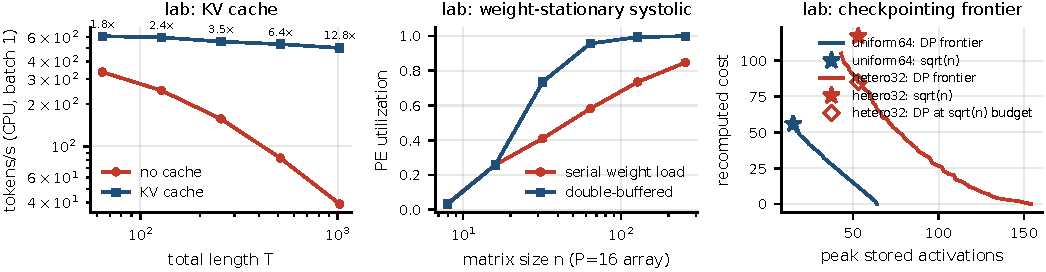
\includegraphics[width=\textwidth]{fig_lab_kv_systolic}
\caption{本文配套实验（CPU 测量与寄存器级仿真）。左：本地训练的 0.8M 参数 nanoGPT（4 层、宽 128）在 CPU、batch 1 下有无 KV cache 的生成吞吐。加速比从 $T=64$ 的 1.8 倍增长到 $T=1024$ 的 12.8 倍，
因为没有 cache 时每一步都要重算整个前缀，总代价是 $O(T^2)$。中：$16\times16$ weight-stationary systolic 阵列的 PE 利用率随矩阵尺寸的变化；权重双缓冲在 $n\ge64$ 时把利用率推到 0.95 以上，因为加载权重的周期被藏到了计算后面。
右：激活重计算的「峰值存储--重算代价」前沿，星号是 $\sqrt{n}$ 均匀分段，菱形是同一预算下动态规划的解。}
\label{fig:labkvsys}
\end{figure*}

\begin{qa}{Systolic array 为什么适合矩阵乘？缺点是什么？}
\ans 因为矩阵乘里每个操作数都要参与 $O(n)$ 次运算，systolic 阵列让这种复用发生在相邻 PE 的寄存器之间：从 SRAM 读一次的数被用 $P$ 次，
控制逻辑又极少，所以能效很高。缺点有两个。矩阵比阵列小或形状不匹配时，$3P-2$ 的填充排空开销摊不薄，利用率低；
对 softmax、归约、gather 这类非 GEMM 运算也不友好，需要额外的向量和标量单元。
\wrong 「TPU 快是因为频率高」。TPU v1 的频率只有 700~MHz。
\end{qa}

\begin{qa}{weight-stationary 和 output-stationary 怎么选？}
\ans 看哪个操作数复用最多、哪个最大。推理时同一份权重要乘 batch 里的每个样本，让权重常驻就能把权重读取摊到整个 batch 上，适合 batch（$M$）大的场景。
output-stationary 让部分和一直留在 PE 里，省掉部分和的往返，适合收缩维 $K$ 很长、输出较小的场景。
\wrong 「两者只是实现细节，性能一样」。
\end{qa}

\subsection{TPU：从推理 ASIC 到光互联超级计算机}

TPU v1~\cite{jouppi2017tpu} 是一颗推理芯片：$256\times256=65536$ 个 8 位 MAC，频率 700~MHz，峰值约 92~TOPS；
片上有 28~MiB 软件管理的存储（24~MiB unified buffer 加 4~MiB 累加器），权重来自 8~GiB 的 DDR3，带宽 34~GB/s。
这篇论文最有价值的部分不是峰值，而是它的 roofline 分析。线上负载以 MLP 和 LSTM 为主，它们的权重复用程度取决于 batch；
而 P99 时延约束（MLP0 为 7~ms）限制了 batch 不能太大。结果大多数应用都落在 roofline 的斜线段上，受权重带宽限制，只有 CNN 接近计算屋顶。

\begin{est}{TPU v1 的拐点与所需 batch}
峰值是 $65536\times2\times700\,\text{MHz}\approx92$~TOPS，权重带宽 34~GB/s，拐点就是 $92\times10^{12}/34\times10^{9}\approx2700$~ops/B。
INT8 的 MLP 在 batch 为 $B$ 时，每个权重字节做 $2B$ 次运算，所以要 $B\ge1350$ 才受算力限制。线上的 batch 远小于这个数。
这和今天 LLM decode 受 HBM 带宽限制是同一个现象，只是拐点从 2700 换成了 H100 的 295。
\end{est}

之后的 TPU 走向了大规模训练。TPU v4~\cite{jouppi2023tpuv4} 用光路交换机（OCS）把 4096 颗芯片连成可重构的 3D torus，并加入了面向 embedding 的 SparseCore；
每颗芯片的 BF16 峰值是 275~TFLOP/s，配 32~GiB HBM2，带宽约 1.2~TB/s。它的主要编程接口是 XLA 和 GSPMD~\cite{xu2021gspmd}：
程序员给张量加上 sharding 注解，由编译器插入集合通信。

\subsection{AWS Trainium 与 NKI}

Trainium 代表了另一种思路：把片上存储完全交给软件管理。Trainium（Trn1）的 NeuronCore-v2 包含 Tensor Engine（$128\times128$ 的 systolic array）、
Vector Engine、Scalar Engine 和 GpSimd Engine。片上存储分两级：SBUF（24~MiB，分 128 个 partition）存放输入和输出 tile，
PSUM（2~MiB）是矩阵乘的累加缓冲~\cite{awsneuron}。NKI（Neuron Kernel Interface）是一种嵌在 Python 里的 kernel 语言。
在 NKI 中，tile 的第 0 维是 partition 维，最大 128，对应阵列的一条边；\texttt{nc\_matmul} 沿 partition 维做收缩，结果写入 PSUM；
HBM 和 SBUF 之间的搬运全部是显式 DMA。CS149 Fall 2024 的作业 4 就是在这套硬件上手工分块卷积和矩阵乘，体会 tile 形状对利用率的影响。
和 GPU 的 shared memory 不同，这里没有 L1/L2 兜底，所有复用都必须显式写出来，写错了就直接撞上 DRAM 带宽墙。

显式化是有代价的。\lab{CS149 A4}测量了 im2col：它把卷积展开成 GEMM，数据膨胀倍数约为 $K_HK_W/\text{stride}^2$，
ResNet conv1（$7\times7$、stride 2）是 12.25 倍。在 numpy 中，im2col 加 GEMM 仍比逐 tap 的直接卷积快，但 $3\times3$ 层有 73\% 的时间花在拷贝 patch 矩阵上；
$1\times1$ 卷积没有膨胀，直接卷积反而更快。GPU 上的 implicit GEMM 和 Winograd 就是为了避开这种显式膨胀。

\begin{table*}[!t]
\centering
\caption{代表性 ML 加速器对比（数字取自论文与官方文档；拐点 = 峰值 / 片外带宽）}
\label{tab:accel}
\footnotesize
\begin{tabularx}{\textwidth}{@{}l L{2.6cm} L{2.8cm} L{3.0cm} Y Y@{}}
\toprule
加速器 & 计算单元 & 片上存储 & 片外存储与峰值 & 编程模型 & 面试要点 \\
\midrule
NVIDIA H100 SXM~\cite{nvidiah100} & 132 SM，第四代 tensor core & 每 SM 256~KB 寄存器、228~KB shared；50~MB L2 & 80~GB HBM3，3.35~TB/s；989 TF/s BF16 稠密，拐点 295 & CUDA/Triton，SIMT + 异步 TMA/wgmma & 通用性最好；硬件 cache 兜底；拐点右移使更多算子访存受限 \\
Google TPU v1~\cite{jouppi2017tpu} & $256\times256$ INT8 systolic，700~MHz & 28~MiB 软件管理 & 8~GiB DDR3，34~GB/s；92~TOPS，拐点约 2700 & CISC 式大指令，主机经 PCIe 下发 & 推理负载多受权重带宽限制；P99 约束限制 batch \\
Google TPU v4~\cite{jouppi2023tpuv4} & MXU systolic 阵列 + SparseCore & 软件管理 SRAM & 32~GiB HBM2，约 1.2~TB/s；275 TF/s BF16 & XLA/GSPMD，sharding 注解 & 4096 芯片 OCS 可重构 3D torus；SparseCore 服务 embedding \\
AWS Trainium~\cite{awsneuron} & $128\times128$ Tensor Engine + Vector/Scalar/GpSimd & SBUF 24~MiB（128 partition），PSUM 2~MiB & HBM（见官方文档） & NKI：显式 tile、DMA、partition 维 & 无 cache 兜底；PSUM 容量限制输出 tile，进而限制强度 \\
MIT Eyeriss~\cite{chen2016eyeriss} & 168 个 PE 的空间阵列 & 全局缓冲 + PE 本地存储 & DRAM & 配置化数据流 & row-stationary 数据流最小化总能耗 \\
\bottomrule
\end{tabularx}
\end{table*}

表~\ref{tab:accel} 把这些加速器放在一起比较。面试中常见的追问是「那为什么 GPU 仍然是主流」。GPU 用大量线程和寄存器文件做通用调度，
tensor core 只是嵌在 SM 里的小矩阵单元，面积效率不如大阵列；但它对 softmax、归约、gather 和动态形状的容忍度高得多。
ASIC 把大部分面积给了阵列和 SRAM，对编译器和张量形状的要求也就更苛刻。这是通用性和能效之间的取舍，谈不上谁先进、谁落后。

\begin{keypts}
\begin{itemize}
\item 专用化的核心是提高「每次取数的复用次数」；按能耗排序，DRAM 访问 $\gg$ SRAM 访问 $\gg$ 乘加。
\item systolic 阵列的利用率 $\approx M/(M+3P-2)$（串行加载权重时）；大阵列需要大矩阵和权重双缓冲。
\item TPU v1 的教训：拐点约 2700，P99 约束下的线上推理多受权重带宽限制，与今天的 LLM decode 是同一个现象。
\item Trainium/NKI：SBUF 和 PSUM 两级软件管理存储，partition 维 128，显式 DMA；tile 形状受 PSUM 容量约束。
\end{itemize}
\end{keypts}

\begin{research}
\begin{itemize}
\item 对 LLM decode 这类低强度负载，专用加速器应该怎样设计？一个方向是加大片上 SRAM，把权重留在片上（用面积换带宽）；
另一个方向是近存计算。可以用本文的 roofline 计算器估算：要让 8B 模型在 batch=1 时 decode 达到 1000~token/s，需要多大的有效带宽？
\item 设计一个跨加速器的「可移植性」实验：同一个 attention kernel 在 GPU（Triton）和 Trainium（NKI）上的 tile 选择为什么不同？
把差异分别归因到片上容量、partition 约束和异步引擎的数量。
\end{itemize}
\end{research}

\section{编译器与框架}
\label{sec:compiler}

上一节的融合和分块，如果每个模型都要人手写，成本是不可接受的。框架决定了用户怎么写模型，编译器决定了硬件怎么跑它，
两者之间的那一层就是本节的主题。我们从计算图和自动微分讲起，接着讨论图级优化（融合、代数替换）、算子级优化（调度空间与搜索），
以及 PyTorch 2 在 Python 字节码层面捕获计算图的路线，最后专门讨论面试的高频难点：动态形状。

\subsection{从 define-and-run 到 define-by-run}

框架的第一个设计选择是：先构图再执行，还是边执行边构图。DistBelief~\cite{dean2012large} 和 TensorFlow~\cite{abadi2016tensorflow} 采用前者，
也就是静态图（define-and-run），好处是整张图可以统一优化和做分布式放置。PyTorch~\cite{paszke2019pytorch} 采用后者，即时执行（define-by-run），
直接用 Python 控制流表达模型，易用得多，代价是失去了全局优化的机会。JAX~\cite{jax2018github} 走的是函数变换的路线（\texttt{jit}、\texttt{grad}、\texttt{vmap}、\texttt{pmap}），
在 tracing 时得到纯函数的中间表示，再交给 XLA 编译~\cite{xla}。PyTorch 2~\cite{ansel2024pytorch2} 则想两者兼得：保留 eager 语义，在运行时把图捕获下来再编译。

\subsection{自动微分}

不管用哪种框架，训练都离不开自动微分。深度学习用的是反向模式自动微分~\cite{baydin2018automatic}：对标量损失 $\mathcal{L}$ 和 $n$ 个参数，
一次反传就能得到全部梯度，代价只是前向的常数倍；前向模式则需要 $n$ 次。对 GEMM 主导的网络，这个常数约为 2，
因为反向要对输入和对权重各做一次同样大小的 GEMM。训练 FLOPs 的经验公式 $C\approx6ND$ 就是这么来的：前向 $2ND$，反向 $4ND$。
反向模式的代价是必须保存前向的中间激活，训练显存里「激活」这一项就来源于此（第~\ref{sec:train} 节）。

\lab{15-849 编译与压缩}用 numpy 实现了一个反向模式自动微分，包括迭代式的拓扑排序、广播求和以及 softmax-交叉熵。
在两层 MLP 上，梯度与 \texttt{torch} 的最大差 $\le5.6\times10^{-17}$，与中心差分的最大差 $\le2.3\times10^{-10}$。
它还测试了 5000 层的链式乘法：因为拓扑排序是迭代而不是递归实现的，反向不会爆栈。

\begin{qa}{为什么深度学习用反向模式而不是前向模式自动微分？代价是什么？}
\ans 因为输出是一个标量，输入却是 $n$ 维参数。反向模式一次反传就拿到全部梯度，代价约为前向的 2--3 倍；前向模式要跑 $n$ 次（或用 $n$ 维的对偶数）。
代价是要保存前向激活，显存随层数和序列长度线性增长，这才引出了重计算和 offload。反过来，如果输出维度远大于输入，比如要求雅可比矩阵的列，前向模式更好。
\wrong 「反向模式更精确」。两者算出的都是精确导数，差别只在复杂度。
\end{qa}

\subsection{图级优化：融合与代数替换}

有了计算图，编译器就可以在图上做优化：常量折叠、公共子表达式消除、布局变换和融合。XLA 的 HLO 融合把逐元素算子和归约算子合成一个 kernel；
TVM~\cite{chen2018tvm} 的 Relay 层按算子类别（injective、reduction、complex-out-fusable）定下融合规则。
TASO~\cite{jia2019taso} 更进一步，自动生成并验证图替换规则，比如把共享同一输入的两个矩阵乘合成一个更宽的矩阵乘，再用代价驱动的回溯搜索选出替换序列。
融合并不总是划算。\lab{15-849 编译与压缩}的结果是，MLP 块的流量降了 49\%，时间却只降了 16\%（第~\ref{sec:kernel} 节）；
而且融合后寄存器压力变大，还可能降低 occupancy。

\subsection{算子级优化：调度空间与搜索}

图切好之后，每个算子内部的循环怎么排，是另一个问题。Halide~\cite{ragan2013halide} 提出了影响深远的「算法与调度分离」：
算法说明算什么，是一个纯函数定义；调度说明按什么顺序、在哪里、用几个核来算，用的是 \texttt{split}、\texttt{reorder}、\texttt{tile}、\texttt{vectorize}、\texttt{compute\_at} 这些原语。
改调度不会改变结果。TVM 把这个思想推广到张量程序，并用学习出来的代价模型指导搜索~\cite{chen2018tvm}。
Ansor~\cite{zheng2020ansor} 连调度模板也不需要人写了：它自动生成层次化的 sketch，再随机注解、做进化搜索，并用代价模型筛选候选。

\lab{15-849 编译与压缩}在 $2048^3$ 的 GEMM 上搭了一个调度空间，由循环顺序和 $t_m,t_n,t_k$ 组成；代价模型是解析的，
参数取单个 H100 SM 分到的算力和带宽（7.49~TFLOP/s、25.4~GB/s、228~KB）。在 3072 个调度里，只有 8 个落在最优值的 5\% 以内。
最优调度是 5.99~ms，也只达到峰值的 38\%，原因是 C 块的强度 $t_mt_n/(t_m+t_n)=128$ 低于拐点 295。
搜索到 5\% 以内需要评估多少次？随机搜索的中位数是 244、P90 是 649；进化搜索的中位数是 147.5、P90 是 496，大约快 1.65 倍；
按枚举顺序的网格搜索是 434，不过这个数只取决于枚举顺序，参考意义不大。

这个实验还给了我一个方法论上的教训。第一版代价模型误用了整颗 CPU 的参数，结果 1080 个调度都落在 5\% 以内，搜索问题被模型弄得过于简单。
可见代价模型决定了搜索问题有多难，这也是 Ansor 要依赖学习型代价模型和真实测量的原因。

\begin{qa}{TVM/Ansor 和 Triton 的定位有什么不同？}
\ans 两者解决的是不同的问题。TVM 把算法和调度分开，靠搜索为每个算子、每种硬件找调度（Ansor 自动生成 sketch、做进化搜索、用学习的代价模型），目标是「不用人写 kernel」。
Triton 让人写 block 级的程序，编译器负责 block 内的线程映射、访存合并和 shared memory，目标是「降低手写 kernel 的门槛」。
前者是自动调优框架，后者是一门编程语言加编译器。
\wrong 「Triton 是 TVM 的前端」；「Ansor 比 Triton 快」。两者解决的问题不同，没法直接比快慢。
\end{qa}

\subsection{PyTorch 2：TorchDynamo、AOTAutograd 与 TorchInductor}

回到「既要 eager 的易用，又要编译的性能」这个目标。PyTorch 2~\cite{ansel2024pytorch2} 的 \texttt{torch.compile} 由三部分组成。
TorchDynamo 借助 CPython 的帧求值钩子（PEP~523），在字节码层面捕获 FX 图，并为图生成 guard，也就是记录张量形状、dtype 和 Python 对象需要满足的条件。
AOTAutograd 在编译期追踪出前向和反向合在一起的联合图，这样反向也能被优化，并在这里决定哪些激活保存、哪些重算。
TorchInductor 把图降为 GPU 上的 Triton kernel，或者 CPU 上的 C++/OpenMP 代码。
遇到追踪不了的 Python 代码，比如数据相关的控制流、\texttt{.item()}、打印、不支持的第三方库，Dynamo 会发生 graph break：
断点前后变成两张独立的图，中间回到 Python 解释执行，跨越断点的融合机会也就没了。

\begin{qa}{\texttt{torch.compile} 什么时候会 graph break？代价是什么？怎么排查？}
\ans 会切图的情况有：数据相关的控制流（\texttt{if x.sum()>0}）、把张量转成 Python 标量（\texttt{.item()}、\texttt{.tolist()}）、打印和日志、
不支持的 C 扩展或第三方库。代价是每个断点都要回一次 Python，图被切碎以后跨断点的融合消失，还可能引起更多重编译。
排查可以用 \texttt{torch.\_dynamo.explain} 或 \texttt{TORCH\_LOGS=graph\_breaks}；修法是把控制流改写成 \texttt{torch.where} 或 \texttt{torch.cond}，
或者把追踪不了的部分移出编译区域。
\wrong 「compile 之后整个模型就是一张图」。
\end{qa}

\subsection{动态形状}

LLM 的序列长度和 batch 每一步都在变，编译器却偏爱静态形状，因为形状决定了分块方式、循环边界和内存规划。主流的处理策略有三种。
第一种是 padding 加分桶：把长度向上取整到若干个桶，用少量静态形状覆盖全部输入，这是 XLA/TPU 的传统做法，代价是 padding 上浪费的计算。
第二种是符号形状：PyTorch 2 把尺寸表示成符号（SymInt），在 guard 中记录形状之间的约束，只有约束被违反时才重编译~\cite{ansel2024pytorch2}。
第三种是运行时专用化：推理引擎为常见的 batch 大小预先捕获 CUDA Graph，其余情况走 eager 路径。
面试中要能讲清楚三者在编译次数、浪费的计算和 kernel 质量这三方面各自的取舍。

\begin{qa}{动态形状为什么让编译器难做？你会怎么处理变长 batch？}
\ans 因为形状决定了分块、循环边界、内存规划和 kernel 选择，形状一变，静态编译的产物要么失效需要重编译，要么变得次优。
训练时，我会按长度分桶并做打包（packing），减少 padding。推理时，decode 的 batch 维分桶并预先捕获 CUDA Graph；prefill 用 varlen attention，
按 cu\_seqlens 把序列拼接起来，避免 padding。在编译器一侧，用符号形状，并只把真正动态的维度标成动态（\texttt{mark\_dynamic}），免得每来一个新长度就重编译一次。
\wrong 「把所有输入 pad 到最大长度就行」。这会把 $T^2$ 的 attention 计算浪费在 padding 上。
\end{qa}

\begin{table*}[!t]
\centering
\caption{ML 编译器与编程系统对比}
\label{tab:compilers}
\footnotesize
\begin{tabularx}{\textwidth}{@{}l L{2.6cm} L{3.2cm} Y Y@{}}
\toprule
系统 & 输入/抽象 & 核心思想 & 优化手段 & 典型局限 \\
\midrule
Halide~\cite{ragan2013halide} & 图像流水线 DSL & 算法与调度分离 & 手写或自动调度（tile、vectorize、compute\_at） & 领域限于规则 stencil/张量 \\
TVM~\cite{chen2018tvm} & Relay 图 + 张量表达式 & 端到端张量编译，调度原语 & 图级融合 + 模板化调度 + 学习的代价模型 & 依赖调度模板；调优耗时 \\
Ansor~\cite{zheng2020ansor} & 张量表达式 & 无模板的层次化搜索空间 & sketch 生成、随机注解、进化搜索、代价模型 & 搜索时间长；对新硬件需要测量 \\
TASO~\cite{jia2019taso} & 算子图 & 自动生成并形式验证图替换 & 代价驱动的回溯搜索替换序列 & 主要是图级，不生成 kernel \\
XLA~\cite{xla} & HLO（JAX/TF） & 整图编译，静态形状 & 融合、布局、buffer 复用；GSPMD 自动分片 & 动态形状需 padding/分桶 \\
PyTorch 2~\cite{ansel2024pytorch2} & Python 字节码 & 保留 eager 语义的图捕获 & Dynamo guard、AOTAutograd、Inductor 生成 Triton & graph break；重编译 \\
Triton~\cite{tillet2019triton} & block 级 Python kernel & 以 tile 为单位编程 & 编译器负责线程映射、合并访存、shared memory & 需人写算法；跨 block 协作受限 \\
\bottomrule
\end{tabularx}
\end{table*}

把这些系统按时间放在一起看（表~\ref{tab:compilers}），能看到一条清楚的演化线：最早是人写调度（Halide、TVM 模板），然后是机器搜索调度（Ansor），
再到人写 tile 级算法、由编译器负责 tile 内部的映射（Triton），最后是框架自动捕获计算图，并把融合后的子图交给 Triton（PyTorch 2）。
GSPMD~\cite{xu2021gspmd} 和 Alpa~\cite{zheng2022alpa} 把同样的编译思想用到了分布式并行上，第~\ref{sec:train} 节会讲到。

\begin{keypts}
\begin{itemize}
\item 反向模式 AD：一次反传得到全部梯度，代价约为前向的 2 倍（$6ND$ 的来源），但需要保存激活。
\item 图级优化有融合、CSE 和代数替换（TASO）；算子级优化靠算法与调度分离（Halide/TVM）和搜索（Ansor）。
\item \texttt{torch.compile} 由 Dynamo（字节码捕获 + guard）、AOTAutograd（联合前反向图）和 Inductor（生成 Triton）组成；graph break 会切断融合。
\item 动态形状的三种策略：分桶 padding、符号形状、运行时专用化（CUDA Graph）。
\end{itemize}
\end{keypts}

\begin{research}
\begin{itemize}
\item 代价模型的可迁移性：在一类 GPU 上训练的代价模型，能不能迁移到新架构上？可以把本文的解析模型当作「先验」，
只用少量真实测量做校准，衡量搜索到 5\% 以内需要多少次测量。
\item 融合决策应该基于 roofline，而不是简单地「能融就融」。一个可做的研究是把每个候选融合组的收益估计为
$\Delta t=\max(F/P,B/\mathrm{BW})$ 的变化量，再与 Inductor 的启发式规则对比。
\end{itemize}
\end{research}

\section{分布式训练}
\label{sec:train}

分布式训练的全部设计都可以看作在式~\eqref{eq:three} 的三项之间做交换：用通信换显存（ZeRO、FSDP），用计算换显存（重计算），
用显存换通信（梯度分桶、更大的 micro-batch），用气泡换显存（流水线）。本节先建立集合通信的代价模型，
再依次讨论数据并行与 ZeRO、张量并行、序列/上下文并行、流水线并行，最后给出 3D 并行的规划方法与显存优化手段。

\subsection{数据并行与参数服务器}

数据并行（DP）让每张卡持有完整模型、处理不同数据，每步对梯度求平均。早期的 DistBelief~\cite{dean2012large} 与参数服务器~\cite{li2014scaling}
把参数分片放在专门的 server 上，worker 推送梯度、拉取参数，支持异步与有界陈旧（bounded staleness），至今仍用于推荐模型的稀疏 embedding。
稠密模型则转向 all-reduce：Horovod~\cite{sergeev2018horovod} 把百度的 ring all-reduce 引入 TensorFlow，PyTorch DDP~\cite{li2020pytorch}
把梯度按反向顺序分桶（默认约 25~MB），一个桶的梯度就绪即异步发起 all-reduce，与后续层的反向重叠。

\begin{qa}{DDP 怎么让通信与反向重叠？bucket 大小怎么取？}
\ans 梯度按参数注册的逆序分桶，反向时一个桶内全部梯度就绪就异步发起 all-reduce，后面的层继续算反向。桶太小，延迟项 $\alpha$ 与 kernel 数多；
桶太大，最后一个桶的通信暴露在反向结束之后。默认 25~MB 量级，按网络带宽与模型层大小调整；\texttt{find\_unused\_parameters=True} 会破坏重叠。
\wrong 「等反向全部结束再 all-reduce」；或认为 DDP 每个参数单独 all-reduce。
\end{qa}

\subsection{集合通信的 $\alpha$--$\beta$ 模型}

用 $\alpha$ 表示每条消息的固定延迟、$\beta$ 表示每字节传输时间（$1/\beta$ 为单向带宽），消息大小 $S$、参与者 $p$。表~\ref{tab:collectives} 汇总了
常用算法的代价~\cite{thakur2005optimization,patarasuk2009bandwidth}。ring all-reduce 由 reduce-scatter 与 all-gather 两个阶段组成，
各 $p-1$ 步、每步每卡收发 $S/p$：
\begin{equation}
t_{\text{ring}} = 2(p-1)\alpha + \frac{2(p-1)}{p}\,S\beta .
\label{eq:ring}
\end{equation}
带宽项趋近 $2S\beta$，与卡数几乎无关，且是带宽最优的~\cite{patarasuk2009bandwidth}；但延迟项随 $p$ 线性增长。
二项树（reduce + broadcast）的延迟项只有 $2\lceil\log_2p\rceil\alpha$，但每步都传完整消息，带宽项为 $2\lceil\log_2p\rceil S\beta$。
递归减半--倍增（Rabenseifner）同时达到 $\log p$ 的步数与最优带宽项，但对物理拓扑敏感~\cite{thakur2005optimization}。

\begin{table}[!t]
\centering
\caption{集合通信算法的 $\alpha$--$\beta$ 代价（全互联、单端口全双工）}
\label{tab:collectives}
\footnotesize
\begin{tabularx}{\columnwidth}{@{}l c Y@{}}
\toprule
算法 & 步数 & 时间 \\
\midrule
ring reduce-scatter / all-gather & $p-1$ & $(p-1)\alpha+\frac{p-1}{p}S\beta$ \\
ring all-reduce & $2(p-1)$ & $2(p-1)\alpha+\frac{2(p-1)}{p}S\beta$ \\
二项树 all-reduce & $2\lceil\log_2p\rceil$ & $2\lceil\log_2p\rceil(\alpha+S\beta)$ \\
递归减半--倍增 & $2\lceil\log_2p\rceil$ & $2\lceil\log_2p\rceil\alpha+\frac{2(p-1)}{p}S\beta$ \\
naive（root 汇聚 + 广播） & $2(p-1)$ & $2(p-1)(\alpha+S\beta)$ \\
all-to-all（成对交换） & $p-1$ & $(p-1)\alpha+\frac{p-1}{p}S\beta$ \\
\bottomrule
\end{tabularx}
\end{table}

\begin{figure*}[!t]
\centering
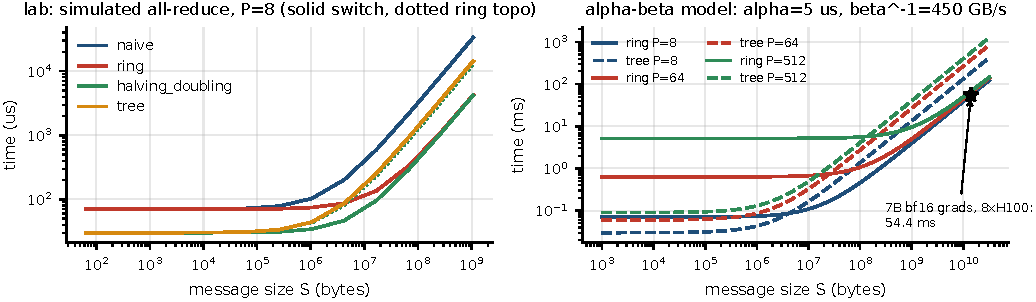
\includegraphics[width=\textwidth]{fig_allreduce}
\caption{all-reduce 时间随消息大小的变化。左：本文配套实验（15-849 分布式训练）的集合通信模拟器，$P=8$，$\alpha=5$~\textmu s，$1/\beta=450$~GB/s；
实线为交换机（全互联）拓扑，虚线为物理环拓扑。所有算法真实搬运 numpy 数组并逐 rank 计字节，模拟时间与闭式公式一致到 $10^{-12}$。
右：闭式 $\alpha$--$\beta$ 模型下 ring 与二项树在 $P=8,64,512$ 时的对比；五角星为 7B 模型 BF16 梯度（14~GB）在 8 卡 NVLink 上的 ring all-reduce（54.4~ms）。
小消息由延迟项主导（树赢），大消息由带宽项主导（ring 赢），交叉点随 $\alpha/\beta$ 与 $P$ 移动。}
\label{fig:allreduce}
\end{figure*}

图~\ref{fig:allreduce} 是这些公式的可视化。\lab{15-849 分布式训练}的模拟器在 $P=8$ 时给出：1~KB 消息 ring 70~\textmu s、树 30~\textmu s；
ring 在约 4.27~MB 处反超树；1~GB 时 ring 4.25~ms、树 14.3~ms；递归减半--倍增在交换机拓扑上与 ring 相当（4.21~ms），但在物理环上因链路争用慢到 12.56~ms，约 3 倍。
$P=64$、1~KB 时 ring 630~\textmu s 而树只有 60~\textmu s——这就是 NCCL 在大规模集群上引入 tree/双二叉树算法的原因。
唯一的真实测量是 CPU 上的 gloo：world=2 时 1~KB 0.40~ms、16~MB 25.8~ms，拟合 $\alpha\approx181$~\textmu s、等效带宽约 0.97~GB/s，只说明数量级。

\begin{est}{7B 模型的梯度 all-reduce 要多久？}
BF16 梯度 $S=2\times7\times10^9=14$~GB。8 卡 H100 节点内 NVLink 单向 450~GB/s，由式~\eqref{eq:ring}，带宽项
$2\times\frac{7}{8}\times14\times10^9/450\times10^9\approx54$~ms（\texttt{mlsys\_calc.ring\_allreduce\_time}，54.4~ms）。
若跨节点走每卡 400~Gb/s（50~GB/s）的 InfiniBand，约 0.49~s。一个 7B 模型在 8 卡上的单步计算若为数百毫秒，
那么跨节点时通信必须与反向重叠（分桶）、或者用分层 all-reduce（节点内 reduce-scatter、节点间 all-reduce、节点内 all-gather）。
\end{est}

\begin{qa}{all-reduce 为什么可以拆成 reduce-scatter + all-gather？这有什么用？}
\ans 先把和按分片算好（每卡得到 $1/p$ 的完整和），再把分片广播给所有人，结果与直接 all-reduce 相同。拆开之后可以只做一半：
ZeRO-2 只需要 reduce-scatter（每卡只更新自己负责的那份参数），ZeRO-3/FSDP 在前向用 all-gather 收集权重，序列并行用 RS+AG 替代 all-reduce
并在中间把激活按序列切分。
\wrong 「all-reduce 是原子操作，不能拆」。
\end{qa}

\begin{qa}{ring 和 tree all-reduce 怎么选？「环越大越慢」对吗？}
\ans ring 的带宽项 $2(p-1)S\beta/p$ 最优且几乎与 $p$ 无关，但延迟项 $2(p-1)\alpha$ 随 $p$ 线性增长；树的延迟项是 $O(\log p)$，带宽项差 $\log p$ 倍。
小消息（延迟主导）用树，大消息（带宽主导）用 ring；NCCL 根据消息大小与拓扑自动选择，并对大消息做分块流水。
\wrong 「ring 总是最好」或「环越大越慢」——变慢的只是延迟项，带宽项不变。
\end{qa}

\subsection{ZeRO 与 FSDP}

混合精度 Adam 的静态显存为每参数 16 字节：BF16 权重 $2N$、BF16 梯度 $2N$、FP32 主权重 $4N$、Adam 一阶矩 $4N$ 与二阶矩 $4N$
（后三项合称优化器状态 $12N$）~\cite{rajbhandari2020zero}。数据并行让每张卡都存一份完整的 $16N$，是巨大的冗余。
ZeRO~\cite{rajbhandari2020zero} 分三级消除冗余（$d$ 为 DP 度）：
\begin{equation}
\begin{gathered}
M_{\text{ZeRO-1}} = 4N+\frac{12N}{d},\qquad
M_{\text{ZeRO-2}} = 2N+\frac{14N}{d},\\
M_{\text{ZeRO-3}} = \frac{16N}{d}.
\end{gathered}
\label{eq:zero}
\end{equation}
ZeRO-1 只切优化器状态，ZeRO-2 再切梯度（reduce-scatter 代替 all-reduce），ZeRO-3 再切权重（前向、反向各 all-gather 一次）。
通信量方面，DP 的 all-reduce 等价于 RS+AG，每卡约 $2\Psi$（$\Psi$ 为参数字节数）；ZeRO-1/2 相同；ZeRO-3 是前向 AG + 反向 AG + 梯度 RS，共 $3\Psi$，
即 DP 的 1.5 倍。PyTorch FSDP~\cite{zhao2023pytorch} 是 ZeRO-3 的工程化实现：以模块为单位（FSDP unit）分片与 all-gather，
预取下一个 unit 的参数以重叠通信，并支持节点内分片、节点间复制的混合分片（HSDP）以降低跨节点流量。

\begin{table}[!t]
\centering
\caption{训练静态显存（GB/卡，不含激活；\texttt{mlsys\_calc.training\_memory\_bytes}）}
\label{tab:trainmem}
\footnotesize
\begin{tabularx}{\columnwidth}{@{}l c Y Y Y Y@{}}
\toprule
模型 & DP & 不切 & ZeRO-1 & ZeRO-2 & ZeRO-3 \\
\midrule
7B（$N=7\times10^9$） & 8 & 112.0 & 38.5 & 26.3 & 14.0 \\
Llama-3-8B（8.03B） & 8 & 128.5 & 44.2 & 30.1 & 16.1 \\
Llama-3-8B & 64 & 128.5 & 33.6 & 17.8 & 2.0 \\
Llama-3-70B（70.6B） & 8 & 1128.9 & 388.1 & 264.6 & 141.1 \\
Llama-3-70B & 64 & 1128.9 & 295.4 & 156.5 & 17.6 \\
\bottomrule
\end{tabularx}
\end{table}

\begin{est}{Llama-3-8B 与 70B 的训练显存}
8B：$16N=16\times8.03\times10^9\approx128.5$~GB，单卡放不下；8 卡 ZeRO-1 为 $4N+12N/8=32.1+12.0=44.2$~GB，ZeRO-3 为 16.1~GB（表~\ref{tab:trainmem}）。
70B：$16N\approx1.13$~TB。即使 64 卡 ZeRO-2 仍需 156.5~GB/卡（因为每卡保留完整 BF16 权重 141~GB），只有 ZeRO-3 或 TP/PP 能把权重切开。
激活另算：按 Korthikanti 等人的估计~\cite{korthikanti2023reducing}，使用 FlashAttention 时每层约 $34sbh$ 字节（$s$ 序列长、$b$ micro-batch、$h$ 隐藏维），
70B（$h=8192$，80 层）一条 4096 序列约 91~GB，全量重计算后只保留每层输入 $2sbh$，约 5.4~GB。图~\ref{fig:trainmem} 给出完整分解。
\end{est}

\begin{figure*}[!t]
\centering
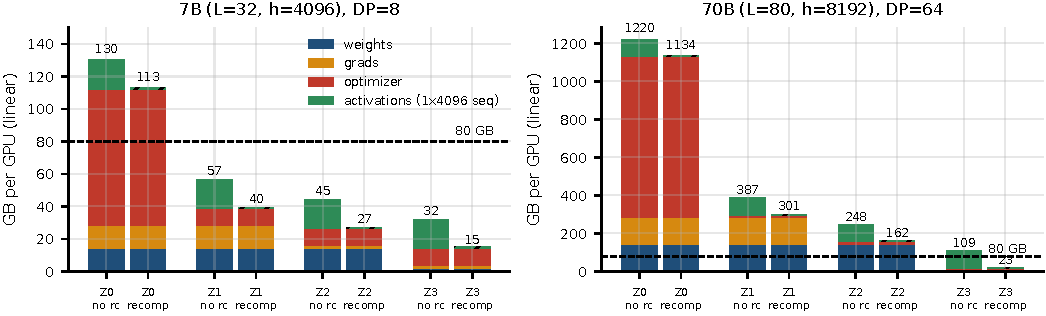
\includegraphics[width=\textwidth]{fig_train_memory}
\caption{每卡训练显存分解：权重、梯度、优化器状态与激活（micro-batch 为 1 条 4096 token 序列，按 Korthikanti 等人的 $34sbh$/层估计，
recomp 表示全量重计算只保留 $2sbh$/层）。左：7B（Llama-2 形状），DP=8；右：70B（Llama-3 形状），DP=64。虚线为 80~GB。
7B 在 ZeRO-1 + 重计算后即可放入单卡（40~GB）；70B 只有 ZeRO-3 才能放下，且激活在 ZeRO-3 下成为最大项（不重计算时 109~GB）。
激活公式针对 GPT 式 $4h$ MLP，对 SwiGLU 只是近似。}
\label{fig:trainmem}
\end{figure*}

\lab{15-849 分布式训练}在 4 个模拟 rank 上用显式的 reduce-scatter/all-gather 实现了 ZeRO 0--3（FP64、分片 Adam），20 步后参数与单进程训练最大差 $2.9\times10^{-16}$；
每 rank 常驻字节是 DP 的 1、0.625、0.4375、0.25（FP64 下 params:grads:m:v=1:1:1:1，理论比例为 $1$、$(2+2/P)/4$、$(1+3/P)/4$、$1/P$），
ZeRO-3 的通信恰好是 DP 的 1.5 倍。按论文的混合精度口径，$\Psi=7.5$B、$N_d=64$ 时计算器给出 120 / 31.4 / 16.6 / 1.88~GB，与 ZeRO 论文图 1 一致~\cite{rajbhandari2020zero}。

\begin{qa}{ZeRO 三个 stage 分别切了什么？通信量变不变？}
\ans stage 1 切优化器状态，stage 2 再切梯度，stage 3 再切权重。1、2 的通信量与 DP 相同（all-reduce=RS+AG，stage 2 只是把 AG 移到参数更新之后），
stage 3 在前向与反向各多一次权重 all-gather，是 DP 的 1.5 倍。7B、8 卡的静态显存依次为 112、38.5、26.3、14~GB。
\wrong 「ZeRO-3 的通信是 DP 的 3 倍」；或「ZeRO 改变了数学，会影响收敛」——它与 DP 数学等价。
\end{qa}

\subsection{张量并行（Megatron-LM）}

Megatron-LM~\cite{shoeybi2019megatron} 把 Transformer 的每一层沿隐藏维切分到 $t$ 张卡。MLP $Y=\mathrm{GeLU}(XW_1)W_2$ 中，$W_1$ 按列切，
每卡得到 $\mathrm{GeLU}$ 输入的一部分列；GeLU 是逐元素的，可本地计算；$W_2$ 按行切，正好消费这部分列，得到部分和，一次 all-reduce 求和。
attention 按头切分，$W_O$ 按行切，同样一次 all-reduce。用共轭算子 $f$（前向恒等、反向 all-reduce）与 $g$（前向 all-reduce、反向恒等）表示，
每层前向 2 次、反向 2 次 all-reduce，每次消息为 $b\cdot s\cdot h$ 个元素，与 $t$ 无关。

\begin{est}{张量并行每步要传多少？}
70B：$h=8192$，每卡一步处理 $b\cdot s=8192$ 个 token，BF16 下每次 all-reduce 的消息为 $8192\times8192\times2\approx134$~MB；每层 4 次、80 层约 43~GB/卡/步。
ring 因子 $2(t-1)/t=1.75$，走 450~GB/s NVLink 约 0.17~s，走 50~GB/s IB 约 1.5~s。这些通信在关键路径上，难以与计算重叠，
所以 TP 留在节点内。\lab{15-849 分布式训练}对 Llama-3-8B（batch 1、$s=8192$、$t=8$）的模型值为每次 67.1~MB、0.331~ms，32 层每步 42.4~ms；
TP 切分前后的前向、输入梯度与参数梯度最大差 $\le8.9\times10^{-16}$。
\end{est}

\begin{qa}{Megatron 的 MLP 为什么第一层按列切、第二层按行切？}
\ans 列切后每卡得到 $XW_1$ 的一部分列，GeLU 逐元素可本地算；行切的 $W_2$ 正好消费这部分列，输出部分和，一次 all-reduce 即可。
整个 MLP 前向只有一次通信。若两层都列切，第二层需要完整的输入，中间必须先 all-gather，通信更多。
\wrong 「两层都按列切更省通信」。
\end{qa}

\begin{qa}{为什么张量并行不出节点，而流水线并行可以跨节点？}
\ans TP 每层前反向共 4 次 $b\cdot s\cdot h$ 的 all-reduce，处在关键路径上、难以重叠，必须走 NVLink（450~GB/s）；PP 只在 stage 边界点对点传激活，
每个 micro-batch 一次 $b\cdot s\cdot h$，量小且可以与计算重叠，走 IB（50~GB/s，约为 NVLink 的 1/9）也可接受。
\wrong 「随便放」或「TP 通信量小所以可以跨节点」。
\end{qa}

\subsection{序列并行与上下文并行}

TP 并没有切分 LayerNorm 与 dropout 的激活，这部分在长序列下很可观。Korthikanti 等人的序列并行（SP）~\cite{korthikanti2023reducing}
在这些区域沿序列维切分，把 TP 的 all-reduce 换成 reduce-scatter + all-gather：通信量相同，激活却按 $t$ 切分。
当序列长到单卡放不下 attention 的输入时，需要上下文并行（CP）：Ring Attention~\cite{liu2023ring} 把序列切到 $c$ 张卡，
$K/V$ 块沿环传递，每卡用 online softmax（式~\eqref{eq:online}）累加，通信与块计算重叠；DeepSpeed-Ulysses~\cite{jacobs2023deepspeed}
则在 attention 前后各做一次 all-to-all，把「按序列切」转换为「按头切」，通信量与 $c$ 无关但并行度受头数限制。

\subsection{流水线并行}

流水线并行（PP）把层切成 $p$ 个 stage，一个 mini-batch 切成 $m$ 个 micro-batch。GPipe~\cite{huang2019gpipe} 先做完全部前向再做全部反向，
PipeDream~\cite{narayanan2019pipedream} 的 1F1B 调度在稳态中交替一个前向与一个反向。填充与排空各需 $p-1$ 个时隙，故两者的气泡比例相同：
\begin{equation}
\text{bubble} = \frac{p-1}{m+p-1},\qquad
\text{bubble}_{\text{interleaved}} = \frac{(p-1)/v}{m+(p-1)/v},
\label{eq:bubble}
\end{equation}
其中交错调度（interleaved 1F1B）让每卡负责 $v$ 个不相邻的虚拟 stage~\cite{narayanan2021efficient}，气泡缩小 $v$ 倍，代价是 $v$ 倍的点对点通信。
1F1B 的真正收益是\emph{激活显存}：在途的 micro-batch 从 $m$ 降到最多 $p$。

\begin{figure*}[!t]
\centering
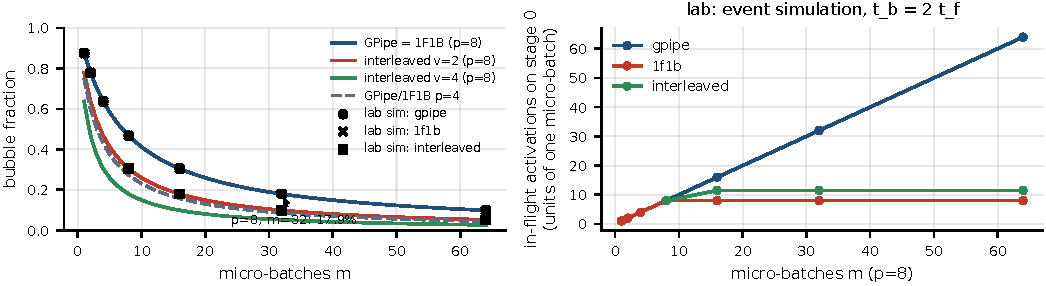
\includegraphics[width=\textwidth]{fig_pipeline}
\caption{流水线气泡与在途激活。左：式~\eqref{eq:bubble} 的气泡比例随 micro-batch 数 $m$ 的变化（$p=8$，$v=1,2,4$；虚线 $p=4$），
黑色标记为配套实验离散事件模拟的结果（$t_b=2t_f$），与公式一致到 $10^{-12}$。$p=8,m=32$ 时气泡为 17.9\%。
右：0 号 stage 的峰值在途激活。GPipe 随 $m$ 线性增长；1F1B 封顶于 $p=8$；交错调度（$v=2$）气泡减半，但在途激活升到 11.5 份，多于 1F1B。}
\label{fig:pipeline}
\end{figure*}

\begin{est}{8 级流水线、32 个 micro-batch 的气泡}
$p=8$、$m=32$：$7/39\approx17.9\%$；$m=8$ 时为 46.7\%，所以经验上取 $m\ge4p$。交错 $v=2$ 时为 9.9\%，$v=4$ 时为 5.2\%
（\texttt{mlsys\_calc.pipeline\_bubble}）。配套模拟中 $p=4,m=8$ 的 GPipe 与 1F1B 气泡都是 0.273，交错 $v=2$ 为 0.158；
但 0 号卡的在途激活 GPipe/1F1B/交错分别为 8/4/5.5 份——气泡与激活显存之间存在真实的权衡（图~\ref{fig:pipeline}）。
\end{est}

\begin{qa}{1F1B 比 GPipe 好在哪？它减少了气泡吗？}
\ans 均匀 stage 下两者的气泡完全相同，都是 $(p-1)/(m+p-1)$。1F1B 在稳态每做一个前向就做一个反向，一个 micro-batch 的反向做完就释放它的激活，
在途激活从 $m$ 份降到 $p$ 份，因此可以用更大的 $m$ 来\emph{间接}降低气泡。真正减小气泡的是交错调度（除以 $v$），代价是 $v$ 倍的点对点通信与更多在途激活。
\wrong 「1F1B 的气泡比 GPipe 小」。
\end{qa}

\subsection{3D 并行的规划}

表~\ref{tab:parallel} 比较了各类并行策略切分的对象、通信模式与适用范围。Narayanan 等人~\cite{narayanan2021efficient} 总结的规划经验可以写成一个可复述的流程：
（1）TP 度 $t$ 取节点内 GPU 数（通常 8），因为 TP 通信量最大且在关键路径上；（2）PP 度 $p$ 取能放下模型的最小值，因为 stage 越多气泡越大；
（3）剩余维度给 DP，并配 ZeRO-1 与梯度分桶重叠；（4）$m\ge4p$ 以控制气泡，同时检查 global batch 不超过收敛允许的临界 batch；
（5）长序列再加 SP/CP，MoE 再加专家并行（第~\ref{sec:eff} 节）。Alpa~\cite{zheng2022alpa} 把算子内（TP/DP）与算子间（PP）并行分层求解，
GSPMD~\cite{xu2021gspmd} 通过 sharding 注解让编译器自动插入通信，它们是「自动并行」的代表。

\begin{table*}[!t]
\centering
\caption{并行策略对比（$N$ 参数量，$s$ 每元素字节，$b\cdot s_{\text{seq}}\cdot h$ 为一个 micro-batch 的激活张量）}
\label{tab:parallel}
\footnotesize
\begin{tabularx}{\textwidth}{@{}l L{2.4cm} L{3.4cm} L{3.6cm} Y@{}}
\toprule
策略 & 切分对象 & 每步通信 & 显存收益 & 适用与代价 \\
\midrule
DP~\cite{li2020pytorch} & 数据 & 梯度 all-reduce，$\approx2Ns$/卡 & 无（每卡完整 $16N$） & 最简单；受 global batch 与显存限制 \\
ZeRO-1/2~\cite{rajbhandari2020zero} & 优化器状态/梯度 & 同 DP（RS+AG） & $4N+12N/d$ / $2N+14N/d$ & 几乎免费的显存收益，默认开启 \\
ZeRO-3 / FSDP~\cite{rajbhandari2020zero,zhao2023pytorch} & 参数、梯度、状态 & $1.5\times$ DP（AG+AG+RS） & $16N/d$ & 模型放不下且不愿改模型代码；跨 IB 时通信重 \\
TP~\cite{shoeybi2019megatron} & 层内权重（隐藏维/头） & 每层 4 次 $bs_{\text{seq}}h$ all-reduce & 权重、梯度、部分激活 $/t$ & 节点内（NVLink）；$t$ 受头数与效率限制 \\
SP~\cite{korthikanti2023reducing} & LayerNorm/dropout 激活（序列维） & 与 TP 相同（RS+AG 替代 AR） & 剩余激活 $/t$ & 与 TP 配合，几乎无额外代价 \\
CP~\cite{liu2023ring,jacobs2023deepspeed} & 序列（attention） & ring 传 K/V 或 2 次 all-to-all & 激活与 attention 输入 $/c$ & 长上下文训练/prefill \\
PP~\cite{huang2019gpipe,narayanan2019pipedream} & 层（stage） & stage 边界点对点 $bs_{\text{seq}}h$ & 权重与状态 $/p$ & 可跨节点；气泡 $(p-1)/(m+p-1)$ \\
EP~\cite{lepikhin2021gshard,fedus2022switch} & MoE 专家 & 每层 2 次 all-to-all（前向） & 专家参数 $/e$ & MoE；负载均衡与 all-to-all 带宽 \\
\bottomrule
\end{tabularx}
\end{table*}

\begin{est}{70B 模型预训练 15T token 需要多少卡、多少天？}
$C=6ND=6\times70.6\times10^9\times15\times10^{12}\approx6.35\times10^{24}$~FLOP。H100、MFU 40\%：1024 卡需
$6.35\times10^{24}/(1024\times989\times10^{12}\times0.4)\approx1.57\times10^7$~s $\approx181$ 天；8192 卡约 23 天（图~\ref{fig:chinchilla} 右）。
显存：TP=8（节点内）$\times$ PP=4 时每卡静态显存 $16N/32\approx35$~GB；再加 DP=256 的 ZeRO-1 为 $4N/32+12N/(32\times256)\approx8.9$~GB，留出空间给激活。
DP 梯度每卡分片 $2N/32\approx4.4$~GB，在 IB 上 ring all-reduce 约 $2\times4.4/50\approx0.18$~s，可藏在反向里。
\end{est}

\begin{qa}{70B 训练为什么不直接用 FSDP/ZeRO-3，而用 TP+PP+DP？}
\ans 两种都可行，取舍在通信位置。ZeRO-3 每层前向、反向都要 all-gather 权重，跨 IB 的总通信是 DP 的 1.5 倍；TP+PP 把每层的大通信留在 NVLink 内，
跨节点只有 PP 的点对点和 DP 的梯度分片。规模越大、网络越慢，TP+PP 越有优势；而 FSDP 的优点是不改模型代码、调度简单，中等规模（数百卡）常常足够。
\wrong 「ZeRO-3 显存最省所以总是最好」。
\end{qa}

\subsection{激活重计算}

Chen 等人~\cite{chen2016training} 提出每 $k$ 层存一个检查点：显存约 $n/k+k$，取 $k=\sqrt{n}$ 时最小约 $2\sqrt{n}$，额外计算约一次前向
（总 FLOPs 从 $3F$ 变为 $4F$，即 $+33\%$）。Checkmate~\cite{jain2020checkmate} 把重计算建模为混合整数线性规划，在显存预算下求最优的保存/重算方案；
Korthikanti 等人~\cite{korthikanti2023reducing} 提出选择性重计算：只重算 attention 中占显存大但计算便宜的部分（softmax、dropout mask），开销仅几个百分点。
\lab{15-849 分布式训练}实现了链上的 $\sqrt{n}$ 与预算约束动态规划：均匀 64 层时 $\sqrt{n}$（每 8 层）峰值 15、重算 56，已在 Pareto 前沿上；
异构 32 层（大小与代价 $\in[1,8]$）在同为 53 的预算下，$\sqrt{n}$ 重算 117 而 DP 只需 85，少 27\%（图~\ref{fig:labkvsys} 右）。
torch 版 16 层实验中 4 层一段（$=\sqrt{16}$）峰值最低，梯度与不重计算逐位相等；CPU 上时间开销 1.52 倍，远高于理论 1.33 倍，是 Python 钩子开销，不能外推到 GPU。

\begin{qa}{激活重计算多花多少算力？}
\ans 全量重计算多一次前向，前向:反向 $=1:2$，总计算从 $3F$ 到 $4F$，即 $+33\%$，不是翻倍。按 $\sqrt{n}$ 设检查点时激活从 $O(n)$ 降到 $O(\sqrt{n})$。
选择性重计算只重算 softmax/dropout 等，开销通常 $<5\%$。报告 MFU 时不计重算 FLOPs，HFU 计入。
\wrong 「重计算让训练慢一倍」。
\end{qa}

\subsection{混合精度、offload 与 FP8}

Micikevicius 等人~\cite{micikevicius2018mixed} 的混合精度训练确立了三件事：FP16 计算、FP32 主权重、动态 loss scaling。
BF16~\cite{kalamkar2019study} 有 8 位指数，与 FP32 动态范围相同，通常不需要 loss scaling，但只有 7 位尾数；
无论哪种，求和、softmax、LayerNorm 统计量与 loss 都应在 FP32 中累加。

ZeRO-Offload~\cite{ren2021zero} 把优化器状态与 Adam 更新放到 CPU，只在 GPU 上做前反向；ZeRO-Infinity~\cite{rajbhandari2021zero} 进一步利用 NVMe。
它们的瓶颈是 PCIe：7B 模型每步向主机传 $2N=14$~GB 梯度、再传回 14~GB 权重，在 32~GB/s 的 PCIe 4.0 上各约 0.44~s，所以 offload
只在单步计算足够长（大 batch）时才划算。

FP8 有 E4M3（精度更高，用于前向权重与激活）与 E5M2（范围更大，用于梯度）两种格式~\cite{micikevicius2022fp8}，H100 上算力是 BF16 的 2 倍。
由于动态范围窄，需要按张量（或更细粒度）缩放，常用 delayed scaling：用前若干步的 amax 历史估计当前 scale。DeepSeek-V3 报告了用细粒度（分块）缩放的
FP8 训练~\cite{deepseekai2024v3}。风险主要在离群值与累加精度，主权重与优化器状态仍为高精度。

\begin{qa}{BF16 和 FP16 训练的区别？FP8 训练要注意什么？}
\ans BF16 有 8 位指数、7 位尾数，范围同 FP32，不需要 loss scaling；FP16 有 5 位指数、10 位尾数，精度更高但梯度容易下溢，必须动态 loss scaling。
两者都要 FP32 主权重与 FP32 累加。FP8 需要 per-tensor/per-block 的 scale（delayed scaling 用 amax 历史），前向用 E4M3、梯度用 E5M2；
注意激活离群值、GEMM 累加精度，以及哪些算子（LayerNorm、softmax、loss）必须留在高精度。
\wrong 「BF16 精度比 FP16 高」；「FP8 训练就是把所有张量转成 8 位」。
\end{qa}

\begin{keypts}
\begin{itemize}
\item ring all-reduce：$2(p-1)\alpha+2(p-1)S\beta/p$；小消息用树、大消息用 ring；7B 梯度 8 卡 NVLink 约 54~ms。
\item $16N$：7B 单卡 112~GB；ZeRO-1/2/3 公式见式~\eqref{eq:zero}；ZeRO-3 通信 1.5 倍。
\item Megatron：列切 + 行切，每层前反向 4 次 $bsh$ all-reduce，留在节点内。
\item 气泡 $(p-1)/(m+p-1)$；1F1B 省激活不省气泡；交错除以 $v$。
\item 重计算 $+33\%$ FLOPs；选择性重计算 $<5\%$；BF16 免 loss scaling；FP8 需要 scale 管理。
\end{itemize}
\end{keypts}

\begin{research}
\begin{itemize}
\item 3D 并行的自动规划（Alpa、GSPMD）通常以静态代价模型为基础，而真实集群的带宽随拓扑与拥塞变化。可做的实验：
在 $\alpha$--$\beta$ 模型中加入拓扑项（交换机 vs 物理环，本文实验显示 halving-doubling 在物理环上慢 3 倍），看最优并行配置是否改变。
\item 流水线调度的「零气泡」方向~\cite{qi2024zerobubble}（把反向拆成对输入与对权重两部分分别调度）与激活显存的关系值得系统测量：
在本文的事件模拟器中把 $t_b$ 拆为 $t_{b,x}+t_{b,w}$，比较气泡与峰值激活的 Pareto 前沿。
\end{itemize}
\end{research}

\section{LLM 推理与服务}
\label{sec:infer}

2023 年以来，LLM 推理是面试中权重上升最快的方向。它和训练最大的区别在于自回归的 decode：每生成一个 token，都要把全部权重和这条序列的全部 KV cache 读一遍，
计算量却只有 $2N$ FLOPs。所以推理的很多问题，归根到底是「每生成一个 token 要读多少字节」的问题。本节先用 roofline 区分 prefill 和 decode，再推导 KV cache 的大小，
然后讨论批处理与调度（continuous batching、PagedAttention、chunked prefill、PD 分离、前缀缓存），最后是推测解码和量化。

\subsection{Prefill 与 decode 的 roofline}

一次请求分两个阶段。prefill 一次处理整段 prompt，线性层是 $[B\cdot T_p, d]\times[d,d]$ 的 GEMM，强度很高，受算力限制，它决定了首 token 时延（TTFT）。
decode 每步每条序列只处理一个 token，线性层退化成 GEMV（batch 为 $B$ 时是 $M=B$ 的瘦 GEMM），受带宽限制，它决定了每 token 时延（TPOT）。
Pope 等人对此做过系统的分析~\cite{pope2023efficiently}。忽略非矩阵运算，一个 decode 步的 roofline 下界是
\begin{equation}
t_{\text{dec}} \approx \max\!\left(\frac{2NB + 4Ld\,TB}{P_{\text{peak}}},\ \frac{sN + \mathrm{KV}(T,B)}{\mathrm{BW}}\right),
\label{eq:decode}
\end{equation}
其中 $4LdTB$ 是 attention 对长度为 $T$ 的上下文做点积和加权求和的运算量，$\mathrm{KV}(T,B)$ 是 KV cache 的字节数（式~\eqref{eq:kv}）。
如果只看权重，强度 $I\approx2NB/(sN)=B$（BF16），也就是说\emph{临界 batch 约等于拐点}，H100 上 $B^\ast\approx295$。
但 KV 的读取不能被 batch 分摊，每条序列都要读自己的 KV，所以长上下文下它会先成为瓶颈。
图~\ref{fig:intbatch} 显示了这一点：上下文为 4096 时，Llama-3-8B 的 decode 强度在大 batch 下趋于约 30；上下文到 32K 时只有约 7，永远到不了拐点。
相比之下，prefill（每条序列 512 token）的线性层强度在 batch 1 时就已经超过 400。

\begin{figure}[!t]
\centering
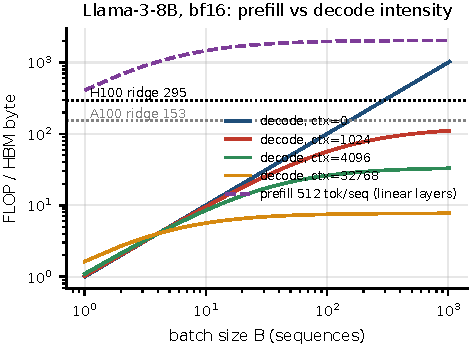
\includegraphics[width=\columnwidth]{fig_intensity_batch}
\caption{Llama-3-8B 在 BF16 下 prefill 与 decode 的算术强度随 batch 的变化（\texttt{mlsys\_calc.decode\_step\_time}）。
不计 KV（ctx=0）时，decode 强度等于 $B$，在 $B\approx295$ 处越过 H100 的拐点；计入 KV 后，强度会饱和在一个由上下文长度决定的常数上，
因为 KV 字节随 batch 同步增长。prefill 的线性层在任何 batch 下都受算力限制。}
\label{fig:intbatch}
\end{figure}

强度饱和意味着吞吐也会饱和。图~\ref{fig:decodetput} 把强度换算成了 decode 吞吐的上界。

\begin{figure*}[!t]
\centering
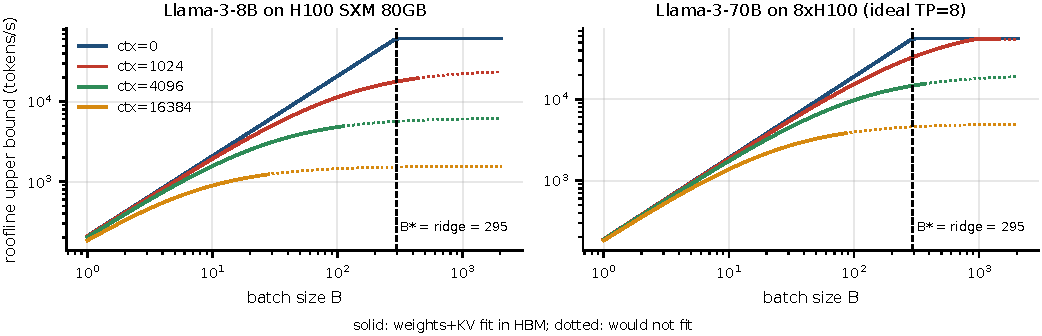
\includegraphics[width=\textwidth]{fig_decode_throughput}
\caption{decode 吞吐的 roofline 上界随 batch 的变化。左：Llama-3-8B，单张 H100；右：Llama-3-70B，理想 TP=8 的 8 卡 H100（聚合算力与带宽，忽略 all-reduce）。
实线表示权重和 KV 能放进 HBM，虚线表示放不下。ctx=0 的曲线在 $B^\ast=295$ 处出现从访存受限到算力受限的拐点；
上下文越长，曲线越早饱和，而且还没到拐点就因为 KV 放不下而终止。也就是说，长上下文下限制吞吐的是 KV 的带宽和容量，而不是算力。}
\label{fig:decodetput}
\end{figure*}

\begin{est}{H100 上 Llama-3-8B 的 decode 上限}
权重 $8.03\times10^9\times2\approx16.06$~GB。batch=1、上下文 4096 时，KV 是 0.54~GB，每步读 16.6~GB，$t\ge16.6/3.35\approx4.95$~ms，约 202~token/s；
而计算只有 $2N\approx16$~GFLOP，只用到峰值的 0.3\%。batch=64 时，KV 是 34.4~GB，每步 15.05~ms，约 4252~token/s，仍然受访存限制。
batch=256 时，KV 达到 137~GB，单卡放不下（\texttt{inference\_math.csv} 与配套实验 CS229S P2 一致）。
作为对比，看短上下文的 7B 模型在 batch=512 时的情况：读权重 14~GB 需要 4.2~ms，计算 $2\times7\times10^9\times512/989\times10^{12}\approx7.2$~ms，
\emph{已经受算力限制}了。RL rollout 这类大 batch 场景里推测解码收益消失，原因就在这里。
\end{est}

\begin{qa}{prefill 和 decode 的瓶颈分别是什么？这对系统设计意味着什么？}
\ans prefill 是 GEMM，受算力限制，决定 TTFT 和算力需求；decode 是 GEMV 或瘦 GEMM，受带宽限制，因为要读全部权重和 KV，它决定 TPOT 以及对显存带宽和容量的需求。
两者混在一起跑会互相干扰：一个长 prefill 会让同批 decode 的 TPOT 抖动。由此引出了两种设计：chunked prefill 把 prefill 切块混进 decode 步；
PD 分离把两者部署到不同的池子里，各自按 TTFT 和 TPOT 选择并行度。
\wrong 「decode 慢是因为计算量大」。
\end{qa}

\subsection{KV cache 的大小}

既然 KV 会成为瓶颈，就得会算它有多大。每一层、每个 token 都要存一个 K 向量和一个 V 向量，长度都是 $n_{kv}\cdot d_{\text{head}}$，所以
\begin{equation}
\mathrm{KV}(T,B) = 2\cdot L\cdot n_{kv}\cdot d_{\text{head}}\cdot T\cdot B\cdot s .
\label{eq:kv}
\end{equation}
代入几个常见模型：Llama-3-8B（$L=32$、$n_{kv}=8$、$d_{\text{head}}=128$）是 128~KiB/token；Llama-3-70B（$L=80$、$n_{kv}=8$）是 320~KiB/token；
没有用 GQA 的 Llama-2-7B（$n_{kv}=32$）是 512~KiB/token~\cite{touvron2023llama,dubey2024llama3}。不同上下文长度下的数值见表~\ref{tab:kv} 和图~\ref{fig:kv}。

\begin{table}[!t]
\centering
\caption{KV cache 大小（BF16，batch=1，单位 GiB；\texttt{mlsys\_calc.kv\_cache\_bytes}）}
\label{tab:kv}
\footnotesize
\setlength{\tabcolsep}{4pt}
\begin{tabularx}{\columnwidth}{@{}l c c Y Y Y@{}}
\toprule
模型 & $n_{kv}$ & KiB/tok & 8K & 32K & 128K \\
\midrule
Llama-2-7B（MHA） & 32 & 512 & 4.0 & 16.0 & 64.0 \\
Llama-3-8B（GQA-8） & 8 & 128 & 1.0 & 4.0 & 16.0 \\
Llama-3-70B（GQA-8） & 8 & 320 & 2.5 & 10.0 & 40.0 \\
70B 若为 MHA（反事实） & 64 & 2560 & 20.0 & 80.0 & 320.0 \\
\bottomrule
\end{tabularx}
\end{table}

\begin{figure}[!t]
\centering
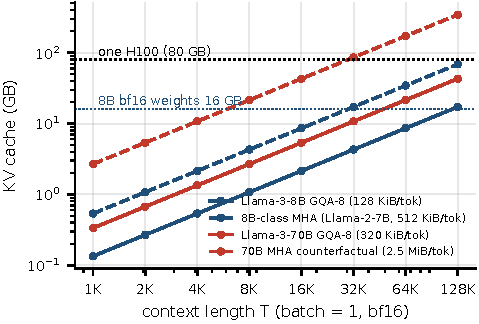
\includegraphics[width=\columnwidth]{fig_kv_cache}
\caption{KV cache 随上下文长度的增长（batch=1，BF16）。实线是采用 GQA-8 的真实模型，虚线是同规模的 MHA。
Llama-3-8B 在 128K 时 KV 为 16~GiB，已经和它 16~GB 的权重相当；70B 如果是 MHA，32K 上下文的一条序列就要 80~GiB，占满一张 H100。
GQA 把 KV 缩小了 $n_{\text{heads}}/n_{kv}$ 倍（8B 是 4 倍，70B 是 8 倍），同样的显存因此能放下长得多的上下文。}
\label{fig:kv}
\end{figure}

\begin{est}{8K 与 128K 上下文的 KV cache}
Llama-3-8B：$2\times32\times8\times128\times2=131072$~B=128~KiB/token。8K 的一条序列是 1~GiB，batch 32 是 32~GiB（34~GB）；128K 的一条序列是 16~GiB。
Llama-3-70B：320~KiB/token，8K 是 2.5~GiB，128K 是 40~GiB，一条 128K 的序列就要占半张 H100。同样条件下，Llama-2-7B 在 8K、batch 32 时需要 128~GiB。
到了 128K，decode 的瓶颈已经从「读权重」变成「读 KV」。KV 量化、GQA/MLA 和上下文并行都是从这里出发的。
\end{est}

\begin{qa}{KV cache 为什么能省计算？它本身的代价是什么？}
\ans 它省掉的是对前缀的重复计算。不缓存时，每一步都要为全部前缀重算 K、V 投影，生成 $T$ 个 token 总共要 $O(T^2)$ 次线性层；缓存之后每步只算新 token，总共 $O(T)$。
配套实验（CS229S P2，CPU）中，$T=1024$ 时 KV cache 把生成速度从 38.9 提到 499~token/s，快了 12.8 倍，总耗时也从 $\sim T^2$ 变成了 $\sim T$。
代价是显存 $2Ln_{kv}d_{\text{head}}TBs$，它决定了最大并发和最长上下文；而且每一步仍要读全部 KV 做点积，attention 的读取量随 $T$ 线性增长。
\wrong 「KV cache 减少了 attention 的计算」；或者计算 KV 大小时用了 $n_{\text{heads}}$ 而不是 $n_{kv}$（GQA 下会差 4--8 倍）。
\end{qa}

\subsection{MQA、GQA 与 MLA}

既然 KV 的大小正比于 $n_{kv}$，最直接的办法就是减少 KV 头。MQA~\cite{shazeer2019fast} 让所有查询头共享一组 K/V，KV 缩小 $n_{\text{heads}}$ 倍，但有质量损失。
GQA~\cite{ainslie2023gqa} 是折中：每组查询头共享一组 K/V，在质量和 KV 大小之间取平衡，而且可以从 MHA 的 checkpoint 经过少量 uptraining 得到。
二者都不改变 attention 的 FLOPs，因为每个查询头仍要和 $T$ 个 key 做点积；它们减少的是 KV 的存储和读取，所以 decode attention 的强度提高了 $n_{\text{heads}}/n_{kv}$ 倍。
DeepSeek-V2 的 MLA~\cite{deepseekai2024v2} 走得更远：它缓存一个低秩压缩的 latent（512 维）加一个解耦的 RoPE key（64 维），推理时把上投影矩阵吸收进查询和输出投影。
论文报告其 KV cache 比 DeepSeek 67B 减少了 93.3\%。

\begin{qa}{GQA、MLA、KV INT8 量化各自省了什么、代价是什么？}
\ans 三者都在减少 KV 的字节，方式不同，而且可以叠加。GQA 减少 KV 头数，KV 和 decode attention 的读取量都减少 $n_{\text{heads}}/n_{kv}$ 倍；它改变了模型结构，需要从训练开始用，或者做 uptraining。
MLA 缓存低秩 latent，压缩比更高，但实现复杂：RoPE 要解耦，还需要能吸收投影矩阵的 kernel。KV INT8/FP8 量化不需要重训，KV 直接减半，代价是轻微的精度损失和反量化开销。
\wrong 「GQA 减少了 attention 的 FLOPs」。
\end{qa}

\subsection{批处理与调度}

decode 受带宽限制，提高吞吐最有效的办法就是把更多请求拼进同一个 batch，让一次权重读取服务更多 token。下面五项技术都在回答同一个问题：怎样在显存和时延约束下把 batch 做大、做稳。

第一项是 continuous batching。传统的静态批处理要等一批里最长的请求生成完，才能换下一批。Orca~\cite{yu2022orca} 提出了 iteration-level 调度：
每个 decode 步都可以让完成的请求离开、让新请求加入；同时用 selective batching，只对线性层拼批，attention 则按请求分别计算。

第二项是 PagedAttention。如果按最大长度给每条序列连续预分配 KV，会产生大量内部碎片和预留浪费。vLLM~\cite{kwon2023vllm} 借鉴了操作系统的分页机制：
KV 按固定大小的块分配（默认 16 个 token 一块），用块表把逻辑块映射到物理块，浪费只发生在最后一块；并行采样和 beam search 还可以通过引用计数和 copy-on-write 共享前缀块。
论文报告的吞吐比当时的系统高 2--4 倍。

第三项是 chunked prefill。Sarathi-Serve~\cite{agrawal2024sarathi,agrawal2023sarathi} 把长 prompt 切成固定预算的块，和 decode 拼在同一步里执行（stall-free batching）。
decode 本来就受访存限制，捎带进去的 prefill 计算几乎是免费的；同时，长 prefill 再也不会让 decode「卡顿」。

第四项是 PD 分离。DistServe~\cite{zhong2024distserve} 和 Splitwise~\cite{patel2024splitwise} 把 prefill 和 decode 放到不同的 GPU 池里，各自选择并行度和 batch，
目标是优化 goodput，即满足 TTFT 和 TPOT 两个 SLO 的请求率。代价是 KV 需要跨卡甚至跨机传输。DistServe 报告，在相同 SLO 下可服务的请求率最高提升了 7.4 倍。

第五项是前缀缓存。SGLang~\cite{zheng2024sglang} 的 RadixAttention 用基数树管理 KV，自动复用不同请求之间共享的前缀，比如系统提示词、few-shot 示例和多轮对话历史；
它还配合缓存感知的调度，优先调度命中前缀较长的请求。

\begin{figure*}[!t]
\centering
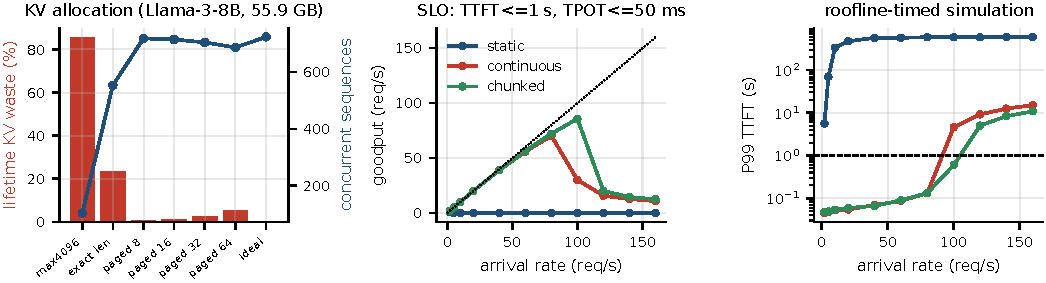
\includegraphics[width=\textwidth]{fig_lab_serving}
\caption{本文配套实验（15-849 服务与显存）中 KV 分配与调度的模拟结果（Llama-3-8B、H100，每步耗时取自 roofline 模型）。
左：10k 个请求（长度服从对数正态分布）在生命周期内的平均 KV 浪费和并发序列数。按 4096 连续预留时浪费 85.6\%、并发 104；即使预先知道最终长度也浪费 23.5\%；分页（block=16）只浪费 1.25\%，并发升到 714。
中：goodput 随到达率的变化（SLO 为 TTFT$\le$1~s 且 TPOT$\le$50~ms），static 的峰值是 0.97~req/s，continuous 是 70.2，chunked 是 85.7。
右：P99 TTFT，虚线是 1~s 的 SLO。所有时延都是模型输出，没有计入 kernel launch 和 CPU 调度开销，绝对值偏乐观；可以引用的是三者的相对关系和拐点位置。}
\label{fig:labserving}
\end{figure*}

这些机制的效果有多大？\lab{15-849 服务与显存}实现了块表、引用计数、copy-on-write fork、swap/recompute 两种抢占方式，以及按块表 gather 的 attention
（结果与连续存储的实现逐元素相等），再用离散事件模拟比较了三种调度（图~\ref{fig:labserving}）。
在饱和负载（$\lambda=160$~req/s）下，吞吐从 static 的 891~token/s 提到 continuous 的 14,050，再到 chunked 的 16,156。
最长的单次迭代从 5448~ms 降到 121~ms，再降到 9.2~ms；$\lambda=100$ 时，三者的 P99 TTFT 分别是 583~s、4.58~s 和 0.595~s。
显存紧张时差别更明显：把 KV 预算压到 6.55~GB、$\lambda=60$ 时，continuous 抢占了 73 次，重算了 26,480 个 prefill token，goodput 跌到 6.9~req/s；
chunked 只抢占了 39 次，goodput 保住了 51.1。分页的浪费也可以在白板上估出来：每条序列最多浪费 block$-1$ 个 token，平均约 block/2，
$8/590\approx1.4\%$，和实测的 1.25\% 吻合。

\begin{qa}{PagedAttention 解决的是什么问题？代价呢？block 大小怎么取？}
\ans 它解决的是 KV 的内部碎片和预留浪费，并没有让 KV 变小。按最大长度连续预留时，平均浪费可以超过 80\%；分页之后浪费只出现在最后一块，还能在并行采样、beam search 和共享前缀之间共用块。
代价是 attention kernel 要按块表间接寻址：块越小，访存越零碎，块表也越大；但块越小，浪费也越少。vLLM 默认取 16，是在浪费和 kernel 效率之间的折中。
\wrong 「PagedAttention 减少了 KV 的大小」。它减少的是浪费，不是 KV 本身。
\end{qa}

\begin{qa}{continuous batching 与 static batching 的区别？chunked prefill 又解决了什么？}
\ans 区别在于组批的时机。static batching 下，一批请求要等最长的那条结束，短请求空等，新请求排队；continuous batching 在每个 decode 步重新组批，吞吐和平均时延都更好。
但它留下了一个问题：新请求的整段 prefill 混进某一步时，这一步会变得很长，同批 decode 的 TPOT 出现明显的尖峰。chunked prefill 给每一步设一个 token 预算，把 prefill 切成块，
本文的模拟中最长的一步因此从 121~ms 降到了 9.2~ms。
\wrong 「continuous batching 就是 batch 更大」。
\end{qa}

\begin{qa}{chunked prefill 和 PD 分离怎么选？}
\ans 看规模和 SLO。chunked prefill 在同一组 GPU 上平滑干扰，部署简单，也不用传 KV，但 prefill 和 decode 只能共用一套并行配置。PD 分离让两个池各自按 TTFT 和 TPOT 选择 TP 和 batch，
规模大、SLO 严格时 goodput 更高；代价是 KV 传输（70B、2K token 的 KV 是 640~MB，在 50~GB/s 上约 13~ms），以及两池容量配比带来的运维复杂度。
所以规模小或 prompt 短时选前者，规模大、prompt 长、SLO 严格时选后者。
\wrong 「PD 分离总是更好」。规模小的时候，两个池都吃不满。
\end{qa}

把上面的知识串起来，就能回答一道典型的系统设计题。

\begin{est}{70B 模型在线推理 100~req/s 需要多少张 H100？}
假设输入 2K、输出 500 token，要求 TTFT P99$<$2~s、TPOT P99$<$50~ms，使用 8$\times$H100 节点、TP=8。
\emph{权重}：$70.6\times10^9\times2=141$~GB，每卡 17.6~GB。\emph{KV 预算}：每卡 $80\times0.9-17.6-4\approx50$~GB；按 TP 切开 KV 头后，每卡每 token 是 40~KiB，整个节点约能放 123 万 token，
大约是 490 条 2.5K 长度的并发序列。\emph{decode}（batch 256、平均上下文 2.5K）：读权重要 $141/(8\times3.35)\approx5.3$~ms，读 KV 要 $256\times2500\times320\,\text{KiB}/26.8\,\text{TB/s}\approx7.8$~ms，
计算要 4.6~ms，所以仍受访存限制，单步约 13~ms；按 50\% 的效率算，每个节点约 1 万 token/s。需求是 $100\times500=5$ 万 token/s，需要约 5 个节点。
\emph{prefill}：每秒 $100\times2\text{K}$ 个 token，需要 $2\times70.6\times10^9\times2\times10^5\approx28$~PFLOP/s；单节点峰值 7.9~PFLOP/s，按 50\% MFU 约为 4，需要约 7 个节点。
合计约 12 个节点、96 张 H100，其中一半以上用于 prefill。最便宜的两项优化是前缀缓存和 FP8。
\end{est}

\begin{qa}{什么时候前缀缓存（prefix caching）最值钱？它的代价是什么？}
\ans 请求之间共享长前缀的时候最值钱，比如固定的系统提示词、few-shot 模板、多轮对话、agent 的工具描述、对同一份文档的多次提问。命中之后，这一段的 prefill 计算和 TTFT 都省掉了。
代价有三点：缓存要占 KV 显存，和并发争抢；需要淘汰策略（LRU，或基于基数树的引用计数）；路由要有亲和性，同一前缀的请求要落到同一个实例上，否则命中率会很低。
\wrong 「前缀缓存会改变模型输出」。命中的是完全相同前缀的精确 KV，输出不变。
\end{qa}

\subsection{推测解码}

batch 小的时候，decode 读一遍权重只产出一个 token，带宽被浪费了。推测解码~\cite{leviathan2023fast,chen2023accelerating} 利用的正是这部分富余：
先用便宜的草稿模型 $q$ 连续提议 $\gamma$ 个 token，再让目标模型 $p$ 用一次前向并行地验证。第 $i$ 个草稿 token 以概率 $\min(1,p(x)/q(x))$ 被接受；
第一次被拒绝时，从残差分布 $\mathrm{norm}(\max(0,p-q))$ 中重新采样，并截断后面的草稿；如果全部被接受，目标模型再多采一个 token。
设每个 token 的接受率为 $\alpha=\sum_x\min(p(x),q(x))=1-\mathrm{TV}(p,q)$（假设各位置独立同分布），那么每次目标前向产生的期望 token 数和加速比为
\begin{equation}
\mathbb{E}[\text{tokens}] = \sum_{i=0}^{\gamma}\alpha^i = \frac{1-\alpha^{\gamma+1}}{1-\alpha},\qquad
S = \frac{\mathbb{E}[\text{tokens}]}{\gamma c + 1},
\label{eq:spec}
\end{equation}
其中 $c$ 是一次草稿前向相对于一次目标前向的成本。分母里的「1」假设验证 $\gamma+1$ 个 token 和生成 1 个 token 一样贵，这在访存受限的 decode 上近似成立。

\begin{figure*}[!t]
\centering
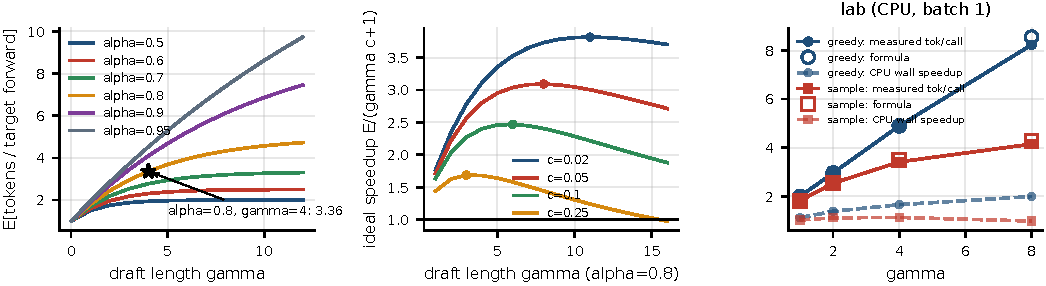
\includegraphics[width=\textwidth]{fig_speculative}
\caption{推测解码。左：式~\eqref{eq:spec} 的期望 token 数随草稿长度 $\gamma$ 和接受率 $\alpha$ 的变化，五角星是 $\alpha=0.8,\gamma=4$ 时的 3.36；$\alpha$ 越高，加长草稿越有用。
中：$\alpha=0.8$ 时理想加速比随 $\gamma$ 和草稿成本 $c$ 的变化，圆点是最优的 $\gamma$：草稿越贵，最优 $\gamma$ 越短，收益也越低。
右：本文配套实验（CS229S P2，CPU，batch 1）中每次目标调用实测得到的 token 数（实心）与公式（空心）相差不到 4\%，但 CPU 上的墙钟加速只有 0.98--1.99 倍。}
\label{fig:spec}
\end{figure*}

\begin{est}{$\alpha=0.8$、$\gamma=4$ 的推测解码}
$\mathbb{E}=(1-0.8^5)/(1-0.8)=(1-0.32768)/0.2\approx3.36$，即每次目标前向平均产出 3.36 个 token。如果草稿成本 $c=0.05$，$S=3.36/(4\times0.05+1)=3.36/1.2\approx2.8$。
从图~\ref{fig:spec} 中图可以读出，$c=0.05$ 时最优的 $\gamma$ 约为 8（$S\approx3.1$），$c=0.25$ 时最优 $\gamma$ 降到 3，$S$ 只有约 1.7。
\end{est}

\lab{CS229S P2}在一个合成语法上训练了 4 层的目标模型（79.7 万参数）和 1 层的草稿模型，实现了采样版的接受--拒绝和贪心版的推测解码，并用显式给出的 $p,q$ 做了 60,000 次试验来检验输出分布。
其中有三个结论值得在面试里讲。第一，贪心版的输出和目标模型逐 token 一致（16/16）。第二，$\alpha$ 的估计方法很容易出错：必须用「接受数 /（接受数 + 拒绝数）」；
如果用「接受数 / 提议数」，第一次拒绝之后那些从未被检验过的草稿也被算进了分母，$\gamma=8$ 时会把 0.80 算成 0.41。
第三，CPU 上验证 $\gamma+1$ 个 token 的一次前向是单 token 前向的 1.41--1.61 倍，草稿的相对成本 $c=0.256$，这是被调用开销抬高的结果，而不是参数比 0.04，
所以墙钟加速只有 0.98--1.99 倍。这个结果不能推出「GPU 上也只有 2 倍」：GPU 上 batch=1 的 decode 受带宽限制，多验证几个 token 几乎不增加时间。

也有方法不用独立的草稿模型。Medusa~\cite{cai2024medusa} 在目标模型上加几个解码头，并行预测后面的若干 token，再用树形 attention 一次验证多条候选；
EAGLE~\cite{li2024eagle} 在特征层（倒数第二层的隐状态）上自回归地生成草稿，接受率更高。但它们仍受同一条约束：只有当验证近乎免费，也就是 decode 受访存限制时，才划算。

\begin{qa}{推测解码为什么不改变输出分布？}
\ans 因为接受和重采样两条路径的概率加起来正好是 $p(x)$。对任意 token $x$，输出它的概率 $=q(x)\min(1,p(x)/q(x))+P(\text{拒绝})\cdot\frac{\max(0,p(x)-q(x))}{\sum_y\max(0,p(y)-q(y))}$。
第一项等于 $\min(p,q)$；拒绝的概率是 $1-\sum\min(p,q)=\sum\max(0,p-q)$，所以第二项等于 $\max(0,p-q)$。两项之和恰好是 $p(x)$。
贪心版则保证输出和目标模型的贪心解码完全相同。
\wrong 「草稿模型猜错的 token 会混进输出」；或者「推测解码是一种近似方法」。
\end{qa}

\begin{qa}{大 batch 下推测解码还划算吗？}
\ans 通常不划算。batch 越大，decode 越接近算力受限（7B 在 batch 512 时已经受算力限制），多验证的 $\gamma$ 个 token 就不再免费。
式~\eqref{eq:spec} 的分母变成 $\gamma c+v$，而 $v$ 会随 batch 增大逐渐接近 $\gamma+1$；同时，被拒绝的 token 白白浪费了算力。所以高吞吐的服务一般只在负载低时打开推测解码，
或者动态调整 $\gamma$。
\wrong 「推测解码在任何负载下都能加速」。
\end{qa}

\subsection{量化}

推测解码是让每次读权重多产出几个 token，量化则是直接减少要读的字节。线性量化把张量映射到 $b$ 位整数网格上。对称量化取 $\text{scale}=\max|x|/(2^{b-1}-1)$，$q=\mathrm{round}(x/\text{scale})$，
误差上界是 scale/2。粒度从粗到细分为 per-tensor、per-channel 和 per-group（$g=64/128$）。
LLM 量化的核心难点是激活离群值：少数固定通道的幅值比其他通道大几十到上百倍~\cite{dettmers2022llmint8}。per-tensor 的 scale 被它撑大以后，其余通道几乎都被量化成了 0。
表~\ref{tab:quant} 汇总了主要的应对方法。

\begin{table*}[!t]
\centering
\caption{LLM 量化方法对比（W$x$A$y$ 表示权重 $x$ 位、激活 $y$ 位）}
\label{tab:quant}
\footnotesize
\begin{tabularx}{\textwidth}{@{}l c L{3.4cm} Y Y@{}}
\toprule
方法 & 典型配置 & 核心思想 & 加速来源 & 代价与局限 \\
\midrule
LLM.int8()~\cite{dettmers2022llmint8} & W8A8 + FP16 离群 & 把幅值超阈值（6）的特征维拆出走 FP16，其余 INT8 & 显存减半 & 混合分解需额外 kernel，吞吐不一定提升 \\
SmoothQuant~\cite{xiao2023smoothquant} & W8A8 & $XW=(X\mathrm{diag}(s)^{-1})(\mathrm{diag}(s)W)$，把激活难度按通道挪到权重 & INT8 tensor core，prefill 与 decode 都受益 & 需要校准；权重也变难量化 \\
GPTQ~\cite{frantar2023gptq} & W4A16/W3A16 & 逐列量化，用 Hessian $H=X^\top X$ 的逆把舍入误差补偿到未量化的列 & decode 读权重字节减少 & 依赖校准数据的协方差；prefill 不加速 \\
AWQ~\cite{lin2024awq} & W4A16 & 按激活幅值找出约 1\% 的显著权重通道，用等价缩放保护 & 同上，硬件友好（无混合精度） & 需要校准；仍是 weight-only \\
QLoRA~\cite{dettmers2023qlora} & NF4 权重 + BF16 LoRA & 4 位 NormalFloat、双重量化、分页优化器 & 微调显存 & 训练吞吐低于 BF16 \\
FP8~\cite{micikevicius2022fp8} & W8A8（E4M3） & 浮点格式自带动态范围，per-tensor/per-block scale & H100 tensor core 2 倍算力 & 需要 scale 管理；仅新硬件支持 \\
\bottomrule
\end{tabularx}
\end{table*}

\begin{figure*}[!t]
\centering
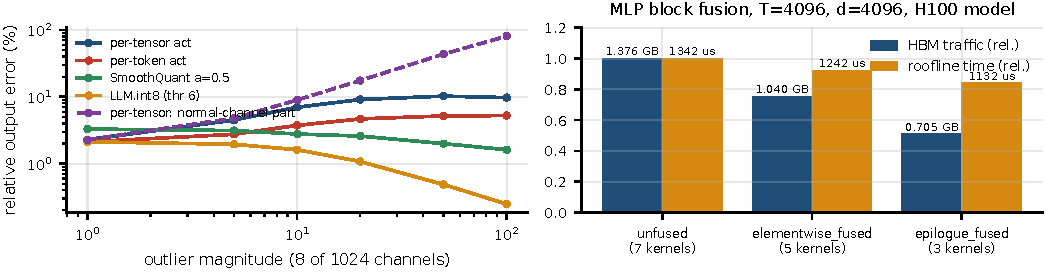
\includegraphics[width=\textwidth]{fig_lab_compress}
\caption{本文配套实验（15-849 编译与压缩）。左：在 1024 个通道中放入 8 个离群通道，W8A8（权重 per-channel）的相对输出误差随离群倍数的变化。
50 倍离群时，per-tensor 激活量化的误差是 10.2\%，per-token 是 5.17\%，SmoothQuant（$\alpha=0.5$）是 1.99\%，LLM.int8 是 0.49\%。虚线显示，per-tensor 下普通通道部分的误差高达 43.6\%（100 倍时 80.8\%）；
整体误差「只有」10\%，是因为离群通道同时主导了输出的范数，掩盖了普通通道的损坏。右：Transformer MLP 块的融合，HBM 流量 $-49\%$，roofline 时间却只有 $-16\%$（第~\ref{sec:kernel} 节）。数据是合成的，用于说明机制。}
\label{fig:labcompress}
\end{figure*}

\lab{15-849 编译与压缩}的激活量化结果见图~\ref{fig:labcompress}。权重量化方面还有两点值得一提。其一，对重尾（Student-$t$）分布的权重，INT8 per-tensor 的误差是 20.6\%，
per-channel 是 1.97\%，group128 是 1.11\%，说明整张表的步长是由一个极大值决定的。其二，GPTQ 只在输入之间有相关性时才有用：输入谱衰减为 1.0 时，测试误差是 3.5\%（RTN 是 25.3\%）；
输入各向同性时反而略差（28.2\% 对 26.4\%）。原因是 $H\approx cI$ 时没有可利用的相关性，补偿项拟合的只是校准集的采样噪声。

\begin{qa}{为什么 LLM 的激活难量化，权重容易？}
\ans 因为离群值集中在激活上。权重近似零均值，离群值少；激活却在少数固定通道上有几十到上百倍的离群值，per-tensor INT8 的 scale 被撑大，普通通道只剩下几个量化级。
离群值是按\emph{通道}出现的，而不是按 token，所以 per-token 量化只能缓解（配套实验中误差减半）。LLM.int8 把离群通道拆出去走 FP16；SmoothQuant 用逐通道缩放把激活的难度挪到权重上。
\wrong 「INT8 对所有张量都一样好做」。
\end{qa}

\begin{qa}{weight-only 量化（W4A16）为什么能加速 decode，却不一定加速 prefill？W4A16 与 W8A8 怎么选？}
\ans 因为两个阶段的瓶颈不同。decode 受带宽限制，读 INT4 权重比 BF16 少 4 倍字节，反量化在寄存器里做，计算本来就不是瓶颈；prefill 受算力限制，权重仍要反量化成 BF16 才能上 tensor core，
算力一点没省，反而多了反量化的开销。所以小 batch、低时延的 decode 选 W4A16；大 batch、prefill 占比高、受算力限制的服务选 W8A8 或 FP8，用上 INT8/FP8 的 tensor core。
\wrong 「量化总是更快」；「4 位一定比 8 位快」。
\end{qa}

\begin{table*}[!t]
\centering
\caption{LLM 服务系统的关键技术对比}
\label{tab:serving}
\footnotesize
\begin{tabularx}{\textwidth}{@{}l L{3.2cm} L{3.6cm} Y@{}}
\toprule
系统/技术 & 解决的问题 & 机制 & 代价与适用条件 \\
\midrule
Orca~\cite{yu2022orca} & 静态批处理的空等与排队 & iteration-level 调度、selective batching & 需要 KV 管理支持动态加入/离开 \\
vLLM~\cite{kwon2023vllm} & KV 碎片与预留浪费 & PagedAttention：块表、引用计数、CoW、抢占（swap/recompute） & kernel 间接寻址；块大小折中 \\
Sarathi-Serve~\cite{agrawal2024sarathi} & prefill 造成 decode 卡顿（TPOT 尖峰） & chunked prefill、stall-free batching、token 预算 & prefill 被切块后 TTFT 略增；预算需调 \\
DistServe~\cite{zhong2024distserve} / Splitwise~\cite{patel2024splitwise} & prefill 与 decode 干扰、并行配置耦合 & PD 分离、按 goodput 规划两池并行度 & KV 跨机传输；容量配比与运维 \\
SGLang~\cite{zheng2024sglang} & 请求间前缀重复计算；结构化程序 & RadixAttention 前缀缓存、缓存感知调度、约束解码 & 缓存占用显存；需要亲和路由 \\
推测解码~\cite{leviathan2023fast,cai2024medusa,li2024eagle} & batch 小时 decode 带宽受限 & 草稿 + 并行验证，分布无偏 & 大 batch 下收益消失；需要草稿模型或额外头 \\
S-LoRA~\cite{sheng2024slora} / Punica~\cite{chen2024punica} & 多 LoRA 适配器服务 & 统一分页、分段 gather-matmul（SGMV） & 异构 rank 的 kernel 效率 \\
\bottomrule
\end{tabularx}
\end{table*}

表~\ref{tab:serving} 把本节讨论过的服务技术放在一起。它们几乎都在应对同一个约束：decode 受带宽和 KV 容量限制，prefill 受算力限制，而在线服务又要同时满足 TTFT 和 TPOT。
面试中的系统设计题（比如上面的 70B 估算）考的就是能否按收益给这些技术排序。一个合理的顺序是：先上 continuous batching 和 PagedAttention，
再做量化和前缀缓存，然后是 chunked prefill 或 PD 分离，最后才是推测解码。

\begin{keypts}
\begin{itemize}
\item decode 步时 $\approx\max(2NB/P,\ (sN+\mathrm{KV})/\mathrm{BW})$；临界 batch 约等于拐点（H100 约 295），但 KV 不能被 batch 分摊。
\item KV $=2Ln_{kv}d_{\text{head}}TBs$：8B 是 128~KiB/token，70B 是 320~KiB/token；8B 在 8K 时 1~GiB，128K 时 16~GiB。
\item 调度的演进：continuous batching、PagedAttention、chunked prefill，再到 PD 分离和前缀缓存。
\item 推测解码 $\mathbb{E}=(1-\alpha^{\gamma+1})/(1-\alpha)$，$\alpha=0.8,\gamma=4$ 时为 3.36；输出分布无偏；大 batch 下不划算。
\item 激活离群值按通道出现；W4A16 加速 decode，W8A8/FP8 加速 prefill。
\end{itemize}
\end{keypts}

\begin{research}
\begin{itemize}
\item 本文的模拟显示，chunked prefill 的吞吐优势有一部分来自 roofline 假设下「混合步完美重叠」。真实 GPU 上混合步的效率是多少？
可以在真实引擎中固定 decode batch，改变捎带的 prefill token 数，测量步长时间与 $\max(F/P,B/\mathrm{BW})$ 的偏差。
\item 推测解码的接受率 $\alpha$ 并不是独立同分布的，它随位置、温度和领域变化。一个可做的实验是按位置统计接受率，检验式~\eqref{eq:spec} 的偏差，
并据此设计自适应 $\gamma$ 的策略。评估指标必须是同一负载下的 goodput，而不是 batch=1 时的加速比。
\end{itemize}
\end{research}

\section{模型效率与架构}
\label{sec:eff}

前几节都把模型当作给定的，只改系统。这一节反过来，讨论通过「改模型」来改变系统代价的方法：参数高效微调、剪枝与蒸馏、混合专家（MoE）、
attention-free 架构，以及决定「训多大的模型、用多少数据」的 scaling law。面试中这部分考的不是算法细节，而是每种方法把式~\eqref{eq:three} 的哪一项换成了哪一项。

\subsection{参数高效微调：LoRA 与 QLoRA}

全量微调一个大模型，显存主要花在梯度和优化器状态上。LoRA~\cite{hu2022lora} 的做法是冻结预训练权重 $W\in\mathbb{R}^{d\times k}$，只训练一个低秩的增量：
\begin{equation}
W' = W + \frac{\alpha}{r}BA,\quad A\in\mathbb{R}^{r\times k},\ B\in\mathbb{R}^{d\times r},\ B_0=0,
\end{equation}
可训练参数只有 $r(d+k)$ 个；推理时可以把 $BA$ 合并回 $W$，不增加时延。$d=k=4096$、$r=16$ 时，可训练参数是 131K，只占全量 16.8M 的 0.78\%。
QLoRA~\cite{dettmers2023qlora} 再把冻结的基座量化成 4 位 NormalFloat（NF4），加上双重量化和分页优化器，使 65B 模型能在单张 48~GB 的 GPU 上微调。

\lab{15-849 编译与压缩}验证了 LoRA 的两个恒等式：初始化时输出与基座的最大差为 0，合并后的最大差是 $3.3\times10^{-15}$。它还验证了低秩逼近的下界：
$d=256$、真实 $\Delta W$ 的秩为 8 时，$r=4$ 的误差 0.434 已经接近 Eckart--Young 下界 0.424，$r=8$ 时降到 0.044。
按 Llama-3-8B 的形状算，$r=8$ 只挂在 q、v 上是 3.41M 参数（0.042\%），$r=16$ 挂在全部线性层上是 41.9M（0.52\%）。

\begin{qa}{LoRA 省的是什么显存？不省什么？}
\ans 省的是梯度和优化器状态。只有 $r(d+k)$ 个参数需要 FP32 主权重和 Adam 的 $m,v$，7B 模型的优化器状态可以从 84~GB 降到 0.1~GB 的量级。
不省的是基座权重和激活：BF16 的基座仍要 $2N$（QLoRA 用 4 位把它降到约 $0.5N$），反向传播也仍要流经全部层。
\wrong 「LoRA 省了前向显存」，或者「LoRA 让训练快很多」。它的前反向计算量和全量微调相近。
\end{qa}

\subsection{剪枝、稀疏与蒸馏}

剪枝想直接减少参数，难点在于稀疏能不能在硬件上兑现成加速。Deep Compression~\cite{han2016deep} 用剪枝、量化（权重共享）和 Huffman 编码，把 CNN 压缩了一到两个数量级；
但非结构化的稀疏在 GPU 上很难变成实际加速。NVIDIA 的 2:4 结构化稀疏（每 4 个元素保留 2 个）由 Ampere 之后的稀疏 tensor core 直接支持，理论算力翻倍~\cite{mishra2021accelerating}。
SparseGPT~\cite{frantar2023sparsegpt} 把 GPTQ 式的二阶补偿用到了一次性剪枝上。知识蒸馏~\cite{hinton2015distilling} 则用大模型的软标签训练小模型，是部署侧最常用的「改模型」手段之一。

结构约束是有代价的。\lab{15-849 编译与压缩}中，对一个 $1024^2$ 的重尾矩阵剪掉 50\%，非结构化剪枝的输出误差是 20.4\%，2:4 是 29.0\%，4:8 是 25.1\%。
在一个小 MLP 上，2:4 稀疏不微调时准确率是 62.9\%，微调 3 轮后回到 67.2\%（稠密模型是 66.2\%）。这说明结构约束越强，就越依赖恢复训练。

\begin{qa}{2:4 稀疏和非结构化稀疏怎么选？}
\ans 在精度和能否加速之间取舍。非结构化稀疏在同样稀疏度下精度更好，但访存不规则、索引开销大，GPU 很难加速。2:4 有硬件支持（稀疏 tensor core，每 4 个元素用 2 位元数据），
能兑现约 2 倍的算力上限，但约束更强、精度损失更大，通常要微调来恢复。实际加速还要看 GEMM 是否受算力限制：decode 受带宽限制时，2:4 省下的是权重字节，而不是 FLOPs。
\wrong 「剪掉 50\% 就快 2 倍」。非结构化的 50\% 在 GPU 上几乎不会变快。
\end{qa}

\subsection{混合专家（MoE）与专家并行}

能不能让参数变多，而每个 token 的计算不变？这就是 MoE 的想法。Sparsely-gated MoE~\cite{shazeer2017outrageously} 用一个门控网络为每个 token 选出 top-$k$ 个专家（每个专家是一个 FFN），
于是参数量随专家数 $E$ 线性增长，每 token 的 FLOPs 却只随 $k$ 增长。GShard~\cite{lepikhin2021gshard} 用 top-2 门控和自动分片把 MoE 扩展到了 600B 参数；
Switch Transformer~\cite{fedus2022switch} 进一步简化为 top-1，并引入了容量因子和辅助负载均衡损失。容量因子规定每个专家最多接收 $\text{capacity}=\text{factor}\times\text{tokens}/E$ 个 token，
溢出的 token 被丢弃或走残差连接。

专家并行（EP）把专家分到不同的卡上，每层前向需要两次 all-to-all，一次把 token 分发给专家（dispatch），一次把结果收回来（combine），反向还要再两次。
DeepSpeed-MoE~\cite{rajbhandari2022deepspeed} 从推理系统的角度优化 MoE；MegaBlocks~\cite{gale2023megablocks} 用块稀疏 kernel，避免了容量因子带来的丢 token 和 padding。
DeepSeek-V2/V3~\cite{deepseekai2024v2,deepseekai2024v3} 采用了细粒度专家加共享专家的结构。

\begin{est}{MoE 的 all-to-all 每次要传多少？}
每张卡 8192 个 token、$d=4096$、top-2、BF16、EP=8：每张卡每次发送 $\approx8192\times2\times4096\times2\times\frac{7}{8}\approx117$~MB。
每层前向 2 次、反向 2 次；如果跨 IB（50~GB/s），每次约 2.3~ms，32 层每步约 0.3~s，和 TP 的通信是同一个量级。所以 EP 通常放在节点内，或者和 DP 交织，以利用节点内的带宽。
\end{est}

\begin{qa}{MoE 为什么「参数多但不贵」？它贵在哪？}
\ans 不贵的是 FLOPs：每个 token 只经过 top-$k$ 个专家，计算量随 $k$ 增长，而不是随 $E$。贵的地方有三处。一是显存，全部专家都要放下，部署时要按总参数而不是激活参数来配卡。
二是通信，EP 每层前反向共 4 次 all-to-all，对网络拓扑很敏感。三是负载不均，热门专家所在的卡会拖慢整步，需要负载均衡损失、容量因子，或者无丢弃的块稀疏实现。
推理时还有一点：decode 读的是被激活专家的权重，batch 一大，几乎所有专家都会被激活，访存上的优势也就随之减少。
\wrong 「MoE 省算力，所以训练和部署都便宜」。
\end{qa}

\subsection{Attention-free 与状态空间模型}

第~\ref{sec:infer} 节看到，长上下文下 KV cache 是 decode 的主要负担。Transformer~\cite{vaswani2017attention} 的 attention 让 KV cache 随长度线性增长，
而循环形式的模型每一步的状态大小是固定的，这正是 attention-free 架构吸引人的地方。线性 attention~\cite{katharopoulos2020transformers} 把 $\mathrm{softmax}(QK^\top)V$
换成 $\phi(Q)(\phi(K)^\top V)$，复杂度降到 $O(Td^2)$。S4~\cite{gu2022efficiently} 用结构化状态空间模型，训练时写成长卷积的形式来并行。
Hyena~\cite{poli2023hyena} 用隐式参数化的长卷积加门控来替代 attention。Mamba~\cite{gu2023mamba} 引入了随输入变化的选择性状态空间，用硬件感知的并行扫描来训练；
推理时每个 token 的代价是 $O(1)$，没有 KV cache。

\lab{CS229S P1}有两个与此相关的测量。第一个是 depthwise 因果卷积的三种写法（$C=16$，float64）。FFT 的耗时只取决于 $N$，$N=16384$ 时约 14--15~ms；
$O(NK)$ 的直接写法随 $K$ 线性增长，其中移位相加在 $K\approx16$ 处、滑窗在 $K\approx64$ 处与 FFT 交叉。所以短卷积（Mamba/H3 的 $K=4$）直接写快 5.2--8.5 倍，
而长卷积（Hyena 的 $K=N$）在所有 $N$ 上都是 FFT 更快。
第二个是 associative recall。一个手工设定权重、没有经过训练的两层 attention-only 模型（一个「上一 token」头加一个匹配头，也就是 induction head）
就能精确地解这个任务：$\beta\ge8$ 时，32 个键值对的准确率是 1.0；$\beta=1$ 时只有 0.227。这说明 attention 天然擅长精确检索；
而状态大小固定的 SSM 必须把历史压缩进状态里，这正是它在 recall 类任务上的弱点。

\begin{qa}{Mamba/SSM 相对 Transformer 的推理优势是什么？代价呢？}
\ans 优势是状态大小固定。写成递归形式时，decode 不需要随长度增长的 KV cache，每个 token 的代价是 $O(1)$，长序列、大 batch 下吞吐和显存都更好；训练时则用并行扫描或卷积形式来并行。
代价是固定大小的状态是对历史的有损压缩，精确检索（长距离复制、associative recall）不如 attention。所以出现了把 attention 和 SSM 混合起来的架构。
\wrong 「SSM 在所有任务上都比 attention 好」，或者「SSM 训练时也是每 token $O(1)$，没法并行」。
\end{qa}

\subsection{Scaling law 与计算最优}

最后一个问题是：给定一笔算力，应该训多大的模型、用多少数据？Kaplan 等人~\cite{kaplan2020scaling} 发现，损失随参数量 $N$、数据量 $D$ 和算力 $C$ 呈幂律下降。
Chinchilla~\cite{hoffmann2022training} 在固定算力下重新做了拟合，结论是参数和数据应该大致同比例增长，约为每个参数 20 个 token：
\begin{equation}
C\approx6ND,\quad D^\ast\approx20N^\ast\ \Rightarrow\ N^\ast\approx\sqrt{C/120}.
\end{equation}
要注意，这是\emph{训练}算力最优，而不是推理成本最优。要大规模部署的模型常常远超 20 token/参数：Llama-3-8B 训了 15T token，约 1868 token/参数~\cite{dubey2024llama3}，
相当于用更多的训练算力换一个更小、推理更便宜的模型。图~\ref{fig:chinchilla} 左把若干公开模型放在 Chinchilla 曲线旁边：GPT-3 175B 只训了 300B token（约 2 token/参数），明显「欠训」；
Chinchilla 70B 落在曲线上；Llama 系列则大幅「过训」。

\begin{figure*}[!t]
\centering
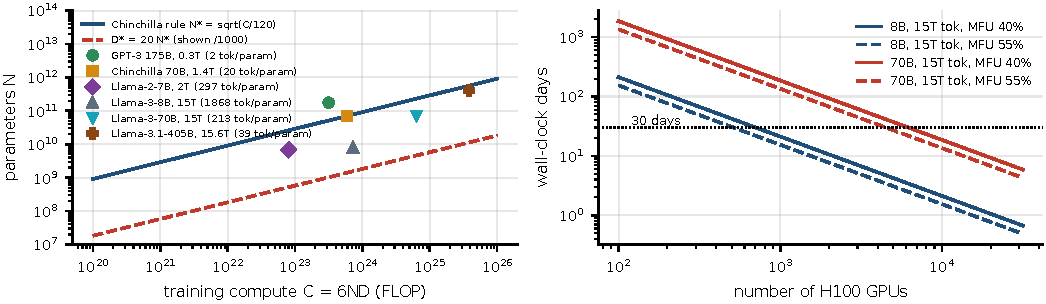
\includegraphics[width=\textwidth]{fig_chinchilla}
\caption{左：Chinchilla 计算最优规则 $N^\ast=\sqrt{C/120}$（实线）与 $D^\ast=20N^\ast$（虚线，缩小 1000 倍显示），以及公开模型的 $(C,N)$ 和 token/参数比；离曲线越远，说明这个模型的训练越偏离「训练算力最优」。
右：在 H100 上用 15T token 训练 8B 和 70B 模型所需的墙钟天数随 GPU 数的变化（MFU 取 40\% 和 55\%）。70B 用 8192 卡、MFU 40\% 时约需 23 天。}
\label{fig:chinchilla}
\end{figure*}

\begin{est}{给定 $6\times10^{23}$ FLOP，计算最优的模型多大？}
$N^\ast=\sqrt{6\times10^{23}/120}\approx7.1\times10^{10}$，也就是约 70B；$D^\ast=20N^\ast\approx1.4$T token。这和 Chinchilla 70B/1.4T 一致（$6\times70\times10^9\times1.4\times10^{12}\approx5.9\times10^{23}$）。
如果改训 8B 模型，同样的算力可以训约 12T token，推理成本约为 70B 的 1/9。用 1 万张 H100、MFU 40\%，$6\times10^{23}$ FLOP 约需 $1.5\times10^5$~s，不到 2 天。
\end{est}

\begin{qa}{Chinchilla 的结论是什么？「每个模型都该训 20 token/参数」对吗？}
\ans 不对，因为 Chinchilla 只考虑了训练算力。它的结论是：固定训练算力时，参数和数据应同比例扩展，最优约为 20 token/参数，$C\approx6ND$。
但如果模型要服务大量请求，总成本是训练加推理，而推理成本随模型大小线性增长，所以应该训练更小的模型、喂更多的 token（Llama-3-8B 约 1868 token/参数）。
可用的高质量数据有限，也是一个现实约束。
\wrong 「Chinchilla 说模型训 20 token/参数最好」。这忽略了推理成本和数据约束。
\end{qa}

\begin{keypts}
\begin{itemize}
\item LoRA 的参数量是 $r(d+k)$，省梯度和优化器状态，不省基座权重和激活；QLoRA 再把基座压到 4 位。
\item 2:4 稀疏有硬件支持（约 2 倍的算力上限）；非结构化稀疏难以兑现加速。
\item MoE：FLOPs 随 $k$ 增长，显存随 $E$ 增长；EP 每层前反向共 4 次 all-to-all（8192 token、$d=4096$、top-2、EP=8 时约 117~MB/次）。
\item SSM：decode 每 token $O(1)$，没有 KV，但精确检索弱；短卷积直接算，长卷积用 FFT。
\item Chinchilla：$N^\ast=\sqrt{C/120}$、$D^\ast=20N^\ast$；要部署的模型常常故意过训。
\end{itemize}
\end{keypts}

\begin{research}
\begin{itemize}
\item 推理感知的 scaling law：把部署时的 token 总量 $D_{\text{inf}}$ 纳入目标函数 $\min_{N,D}6ND+2ND_{\text{inf}}$（在损失约束下），最优的 token/参数比怎样随 $D_{\text{inf}}$ 变化？
这是一个可以用公开拟合系数来做的解析练习。
\item MoE 的通信与计算之比随专家粒度变化：细粒度专家增加了 all-to-all 的消息数（$\alpha$ 项），但改善了负载均衡。可以在本文的 $\alpha$--$\beta$ 模拟器上扫描专家数和 top-$k$，
找出 all-to-all 从带宽主导转为延迟主导的拐点。
\end{itemize}
\end{research}

\section{集群、可靠性与数据}
\label{sec:cluster}

把单个作业的并行策略调好以后，大模型训练的真实效率还受三件事影响：多个作业怎样共享集群（调度），万卡规模下的故障怎样才不会吞掉训练进度（可靠性），
以及 GPU 是不是在等数据（数据管线）。这一层是训练 infra 岗位高级面试题的主要来源。

\subsection{深度学习集群调度}

深度学习作业和传统的批处理作业很不一样。Jeon 等人分析微软 Philly 集群~\cite{jeon2019analysis} 后发现：分布式训练需要 gang scheduling，即所有 worker 必须同时启动，否则先启动的只能空等；
作业对拓扑局部性很敏感，最好放在同一节点或同一交换机下，而这种局部性约束又让排队时间变长；还有相当比例的作业因为用户错误或故障而失败。
针对这些特点，Gandiva~\cite{xiao2018gandiva} 利用 DL 作业的迭代性做时间片轮转和迁移，并根据运行时的观察调整放置。Tiresias~\cite{gu2019tiresias} 在不知道作业时长的前提下，
按「已获得的服务量 = GPU 数 $\times$ 时间」做二维 LAS（least attained service）调度，降低平均完成时间。
Pollux~\cite{qiao2021pollux} 注意到吞吐和统计效率都会随 batch 变化，于是联合调整每个作业的 GPU 数和 batch size，以 goodput 为优化目标。

\begin{qa}{深度学习集群调度和传统批处理调度有什么不同？}
\ans 主要有四点不同。第一是 gang scheduling：分布式作业的所有 worker 必须同时拿到资源。第二是拓扑敏感：放在同一节点或同一交换机下，会直接影响 all-reduce 的时间。
第三是可抢占和弹性：作业可以依靠 checkpoint 暂停、迁移和伸缩。第四是吞吐与资源不成线性关系：卡数加倍不一定吞吐加倍，batch 变大还会改变统计效率（Pollux）。
\wrong 「按 GPU 数量排队就行」。
\end{qa}

\subsection{大规模训练的故障与恢复}

到了万卡规模，故障就是常态。Llama~3 报告，在约 1.6 万张 H100 上的一段 54 天预训练中，作业共中断了 466 次，其中 419 次是非计划中断；
约 78\% 归因于已确认的硬件问题（GPU 和主机组件），GPU 相关问题是最大的一类。靠自动化恢复，有效训练时间仍然超过了 90\%~\cite{dubey2024llama3}。
MegaScale~\cite{jiang2024megascale} 在 12,288 张 GPU 上，把算法、通信重叠、算子和数据管线的优化，与「深度可观测性」（细粒度监控、心跳、自动诊断和慢节点剔除）结合起来，
达到了 55.2\% 的 MFU。Gemini 技术报告~\cite{geminiteam2023gemini} 也讨论了大规模训练中的静默数据损坏（SDC）和快速恢复。

\begin{est}{万卡训练多久坏一次？checkpoint 应该多久存一次？}
设单卡的年故障率是 2\%，1 万张卡每年约坏 200 次，平均约 44 小时一次；再算上网络、主机和软件故障，实际往往是十几小时一次。
70B 模型的完整 checkpoint（BF16 权重加 FP32 主权重和 Adam 状态）约为 $16\times70.6\times10^9\approx1.1$~TB。
Young 公式~\cite{young1974first} 给出最优的保存间隔 $\tau\approx\sqrt{2\delta M}$，其中 $\delta$ 是一次保存的开销，$M$ 是平均故障间隔。
取 $\delta=30$~s、$M=12$~h，$\tau\approx\sqrt{2\times30\times43200}\approx1610$~s，也就是约 27 分钟存一次；每次故障平均损失约 $\tau/2$，再加上重启的时间。
\end{est}

从公式可以看出，工程上的关键是把 $\delta$ 压小。异步 checkpoint 先把分片拷到主机内存，每张卡几 GB，几秒就能完成，训练随即继续，再由后台写入分布式存储；
每个 DP 组只需要保存一份；CheckFreq~\cite{mohan2021checkfreq} 则把快照和持久化组成流水线，并自适应地调整保存频率。
$\delta$ 越小，最优间隔就越短，故障造成的平均损失也越小。

\begin{qa}{checkpoint 间隔怎么定？为什么要异步？}
\ans 间隔要在保存开销和故障损失之间平衡：间隔太短，保存开销占比高；太长，故障时丢的进度多。最小化期望损失，就得到 Young 公式 $\tau\approx\sqrt{2\delta M}$。
异步保存把 $\delta$ 从「写分布式存储的时间」降成「拷贝到主机内存的时间」，既降低了开销，又允许存得更频繁。恢复时间也要考虑：从内存副本（或相邻节点上的冗余副本）恢复，比从远端存储读取快得多。
\wrong 「每 N 步存一次就行」，不考虑故障率和保存开销；或者同步写远端存储，把训练阻塞住。
\end{qa}

\begin{qa}{分布式训练挂住了，你怎么查？}
\ans 挂住几乎总是因为集合通信对不上：某个 rank 少调或多调了一次 collective，或者各 rank 的调用顺序不同。我会这样查。先打开 \texttt{NCCL\_DEBUG=INFO} 和异步错误处理，并设一个合理的超时，
让「挂住」变成「报错」。再用 \texttt{py-spy dump} 看每个 rank 停在哪一行，如果停在不同的 collective 上，就是顺序不一致。常见的根因有：只在 rank 0 执行的分支里调用了 collective；
输入长度不同，导致某个 rank 多跑了一轮；部分参数在某些 rank 上没有梯度。如果只是变慢而不是挂住，就先用 \texttt{nccl-tests} 测 bus bandwidth，与式~\eqref{eq:ring} 的理论值比较，
再检查拓扑（是不是走了 PCIe）和 IB 的配置。
\wrong 「重启一下」或「把超时调大」，却不去定位是哪个 rank 不一致。
\end{qa}

\subsection{性能排查的顺序}

训练或推理变慢时，面试官想听的是\emph{排查的顺序}，以及\emph{能区分不同假设的那个观测}。一个可以复述的顺序是：先用 roofline 算出上界，实测如果已经在上界的 1.2 倍以内，就别再优化 kernel 了；
再看时间线上有没有空洞；然后看单个 kernel 的 DRAM 和 SM 吞吐；最后才调超参，而且每次只动一个变量。表~\ref{tab:debug} 把常见的时间线症状和对应的原因、区分方法列在一起。

\begin{table}[!t]
\centering
\caption{时间线症状、最可能的原因与区分性观测}
\label{tab:debug}
\footnotesize
\begin{tabularx}{\columnwidth}{@{}L{2.2cm} L{2.4cm} Y@{}}
\toprule
时间线上看到的 & 最可能的原因 & 区分它的观测 \\
\midrule
kernel 间大量小空洞 & CPU 发射开销、小 kernel 过多 & 空洞宽度与 kernel 数成正比；CUDA Graph 或 \texttt{torch.compile} 后消失 \\
每步开头一段空白 & dataloader 跟不上 & 加倍 \texttt{num\_workers} 后变短；GPU 空闲时 CPU 满载 \\
反向后一大段 NCCL & 梯度通信未与反向重叠 & bucket 过大或开启了 \texttt{find\_unused\_} \texttt{parameters} \\
周期性长尖峰 & 分配器碎片整理、checkpoint & \texttt{num\_alloc\_retries} 增长 \\
利用率 100\% 但慢 & 访存受限 kernel & DRAM 吞吐近峰值、SM 吞吐低 \\
某卡总是最后到 & 负载不均或慢卡 & 每 rank 步时分布；换卡后是否跟随 \\
\bottomrule
\end{tabularx}
\end{table}

\begin{qa}{MFU 只有 25\%，你怎么查？}
\ans 先算账，再看 profile。算账是指用 $6N$ 加上 attention 项估计模型 FLOPs，并确认 MFU 的分母用的是稠密峰值，不含稀疏。然后按占比从大到小逐项排查：通信有没有暴露（没有和计算重叠的 all-reduce 或 all-gather）；
流水线气泡是不是太大（$m<4p$）；dataloader 有没有造成每步开头的空白；逐元素 kernel 有没有融合；micro-batch 是不是太小，GEMM 吃不满；是不是开了全量重计算（这时 HFU 高而 MFU 低）。
每次只改一个因素，改完重新测。
\wrong 一上来就去手写 kernel，或者只报 HFU。
\end{qa}

\subsection{数据管线}

最后一个容易被忽视的问题是：GPU 会不会在等数据？Mohan 等人~\cite{mohan2021analyzing} 发现，很多训练作业有相当一部分时间耗在「数据停顿」（data stall）上，也就是数据读取和预处理跟不上 GPU。
tf.data~\cite{murray2021tfdata} 用流水化、并行 map 和自动调优来缓解这个问题。LLM 预训练的数据管线以离线预分词、内存映射的二进制分片和按长度打包（packing）为主，在线开销较小；
但多模态（要解码图像和视频）和 RL（要生成 rollout）又把数据这一侧推回了关键路径。

这里还有两个经典系统值得一提。Spark 的 RDD~\cite{zaharia2012resilient} 靠 lineage 重算实现容错，是大规模离线数据处理的基础；参数服务器~\cite{li2014scaling} 则在推荐场景中继续承担稀疏 embedding 的训练。
把这两者和 all-reduce 对照着讲，是 CS149 和 15-849 之间最自然的衔接：它们分别代表了数据并行原语在批处理、稀疏训练和稠密训练中的三种形态。
另一个方向是用学习的方法来优化系统本身，比如用强化学习做设备放置~\cite{mirhoseini2017device}，这对研究岗是加分项。

\begin{keypts}
\begin{itemize}
\item DL 调度的特点：gang、拓扑敏感、可抢占与弹性、吞吐与资源非线性（Gandiva、Tiresias、Pollux）。
\item 万卡训练的故障按小时计；Llama~3 的 54 天里有 419 次非计划中断，约 78\% 是硬件问题。
\item Young 公式 $\tau\approx\sqrt{2\delta M}$；用异步、分片、先写内存再落盘来压小 $\delta$。
\item 排查顺序：先算 roofline 上界，再看时间线空洞，然后看单 kernel 吞吐，最后调超参；训练挂住时先查 collective 的调用顺序。
\end{itemize}
\end{keypts}

\begin{research}
\begin{itemize}
\item 静默数据损坏（SDC）在万卡规模下怎样检测？一个可做的设计是周期性地让不同的 rank 重复计算同一个小批次，并比较梯度的哈希；
需要量化它的开销和检出率之间的权衡。
\item 用本文的事件模拟器研究「慢节点」对同步训练的影响：一个 rank 慢 10\% 时，DP、PP、TP 各自的整体吞吐下降多少？
哪种并行方式对尾部延迟最敏感？
\end{itemize}
\end{research}

\section{面试能力框架}
\label{sec:interview}

前十节是知识；本节把它们组织成面试中可以被观察到的能力。MLSys 面试通常同时考两件事：\emph{工程能力}——能否把一个系统问题拆成可测量、可估算的部分，
并按正确顺序定位瓶颈；\emph{研究能力}——能否读懂一篇论文的真实贡献与前提，提出能区分假设的实验。二者共享同一个底座：
式~\eqref{eq:three} 的三项分解与第~\ref{sec:perf} 节的 roofline。

\subsection{按岗位的能力矩阵}

表~\ref{tab:roles} 按五类常见岗位列出工程与研究两条线上的核心要求、必须当场算出的数，以及面试官最常深挖的方向；
它与图~\ref{fig:map} 的课程分层一一对应：推理岗主要对应第~\ref{sec:infer} 节，训练 infra 对应第~\ref{sec:train}、\ref{sec:cluster} 节，
算子/编译对应第~\ref{sec:kernel}、\ref{sec:compiler} 节，芯片岗对应第~\ref{sec:hw}、\ref{sec:accel} 节。

\begin{table*}[!t]
\centering
\caption{岗位 $\times$ 能力矩阵：工程与研究两条线的核心要求}
\label{tab:roles}
\footnotesize
\begin{tabularx}{\textwidth}{@{}L{2.0cm} Y Y L{3.6cm} L{3.4cm}@{}}
\toprule
岗位 & 工程能力（必须能做） & 研究能力（加分项） & 必须当场算出 & 常被深挖 \\
\midrule
LLM 推理系统 & KV 管理、batching 调度、量化部署、推测解码的工程取舍；读 profile 定位 decode 瓶颈 & 调度策略的理论分析；prefill/decode 分离的建模；新注意力变体的系统代价 & decode 步时、KV 容量、并发上限、TTFT/TPOT & vLLM 分页细节、chunked prefill、SLO 与 goodput \\
训练 infra & DDP/FSDP/3D 并行配置、显存预算、通信重叠、checkpoint 与故障恢复 & 并行策略自动搜索、通信压缩、故障与慢节点建模 & $16N$ 显存、all-reduce 时间、气泡、$6ND$ 天数 & ZeRO 各阶段、TP 为何限在节点内、MFU 排查 \\
算子 / 编译器 & CUDA/Triton kernel、tiling、融合、profile（Nsight） & 调度空间搜索、代价模型、动态形状 & 算术强度、tile 大小、HBM 字节、MFU & FlashAttention IO、bank conflict、occupancy \\
AI 芯片 / 加速器 & 数据流映射、片上存储规划、性能建模与仿真 & 新数据流与稀疏/低精度支持、软硬协同 & PE 利用率、片上带宽、能耗/字节 & systolic 填充开销、TPU 与 GPU 的取舍 \\
MLSys 研究 & 可复现实验、基线公平、消融设计 & 找到被忽视的前提、提出可证伪的假设 & 任一上界估算 & 论文的局限、你会做的下一个实验 \\
\bottomrule
\end{tabularx}
\end{table*}

\subsection{回答模板：结论 → 估算 → 瓶颈 → 权衡 → 证据}

开放式系统题最常见的失败是「列名词」：把知道的技术全部报一遍，却不说哪一个在当前场景下起作用。本文推荐的五步模板强制把回答落到数上：
\begin{enumerate}
\item \textbf{结论}：第一句话直接给判断（「这是带宽受限，先上 GQA 与 INT8 权重」）；
\item \textbf{估算}：用第~\ref{sec:perf} 节的 roofline 与附录的公式给出数量级；
\item \textbf{瓶颈}：说明估算显示的主导项是计算、访存还是通信，以及它会在什么条件下切换；
\item \textbf{权衡}：每个方案的代价（精度、时延、复杂度、显存）；
\item \textbf{证据}：如何测量来验证判断——指出能区分两个假设的那个观测。
\end{enumerate}

\begin{qa}{「把 Llama-3-70B 在线服务的成本降一半」，你怎么答？}
\ans \textbf{结论}：decode 受带宽限制，优先降低每 token 读的字节数，再提高 batch。\textbf{估算}：BF16 权重 141~GB，8 卡 TP 每卡每步读约 17.6~GB，
H100 3.35~TB/s 下约 5.3~ms/步；GQA 下每 token KV 320~KiB。\textbf{瓶颈}：batch 小时权重主导，batch 大、上下文长时 KV 主导。
\textbf{权衡}：INT8/FP8 权重把权重字节减半，精度损失需在任务上验证；FP8 KV 让并发翻倍；推测解码降低时延但大 batch 下收益递减；前缀缓存对系统提示共享的场景收益最大。
\textbf{证据}：先测当前 batch 分布与 KV 占用，若平均 batch 已经很大且 KV 占满，则 KV 量化与前缀缓存优先；若 batch 小，权重量化优先。
\wrong 不做估算直接列「量化、剪枝、蒸馏、FlashAttention、vLLM」。
\end{qa}

\subsection{常见错答}

表~\ref{tab:wrong} 汇总了前文面试追问框中出现频率最高的错答。它们几乎都源于同一个错误：把一个在特定区间成立的结论当成普遍规律，
却不说明区间的边界（batch、序列长度、拓扑、精度）。

\begin{table}[!t]
\centering
\caption{高频错答与纠正}
\label{tab:wrong}
\footnotesize
\begin{tabularx}{\columnwidth}{@{}L{3.0cm} Y@{}}
\toprule
错答 & 纠正 \\
\midrule
FlashAttention 把 attention 变成线性 & FLOPs 不变；HBM 流量 $\Theta(T^2d^2/M)$ 仍二次；显存从 $O(T^2)$ 到 $O(T)$ \\
decode 慢是因为算力不够 & 小 batch 下带宽受限；大 batch、短上下文才转为计算受限 \\
ZeRO-3 通信和 DP 一样 & 约为 DP 的 1.5 倍（多一次前向 all-gather） \\
ring all-reduce 时间随卡数线性增长 & 带宽项 $2(p-1)/p\cdot S/B$ 几乎与 $p$ 无关，延迟项线性 \\
7B 模型训练需要 14~GB & 混合精度 Adam 约 $16N=112$~GB，另加激活 \\
GQA 减少计算 & 主要减少 KV 字节，比例 $n_{\text{heads}}/n_{kv}$ \\
推测解码总能加速 & $\alpha$ 低或大 batch 时可能变慢 \\
MoE 省算力所以便宜 & 显存按总参数，且有 all-to-all 与负载不均 \\
利用率 100\% 说明 GPU 吃满 & 只表示有 kernel 在跑，看 SM 与 DRAM 吞吐 \\
\bottomrule
\end{tabularx}
\end{table}

\subsection{把配套实验变成 STAR 故事}

项目经历是面试中最可控的部分。本文配套仓库的每个实验都按「20 秒结论 → STAR → 白板 → 不能推出的结论 → 追问」组织，
表~\ref{tab:star} 列出了十个故事的结论与考察点。所有数字都来自 CPU 上的测量或解析/离散事件模型，不是 GPU 实测；
讲故事时必须主动说明这一点，并说出「这个实验\emph{不能}推出什么」——这恰恰是面试官判断你是否理解实验的最强信号。

\begin{table*}[!t]
\centering
\caption{本文配套实验的十个 STAR 故事（数字为 CPU 测量或模型输出）}
\label{tab:star}
\footnotesize
\begin{tabularx}{\textwidth}{@{}c L{2.4cm} Y L{3.4cm}@{}}
\toprule
\# & 实验 & 20 秒结论 & 考察点 \\
\midrule
1 & CS229S P1 FlashAttention & 按论文块大小，HBM 流量只比朴素少 2.00 倍（因果 3.7--4.0 倍），在 $T$ 上仍二次 & IO 复杂度、读论文 \\
2 & CS229S P2 推测解码 & 每次目标前向的 token 数与 $(1-\alpha^{\gamma+1})/(1-\alpha)$ 差 4\% 以内；CPU 上加速只有 0.98--1.99 倍 & 推理加速、口径 \\
3 & 15-849 服务 & 连续预留 KV 浪费 85.6\%，分页后 1.25\%，并发 104 → 714；chunked prefill 把最差一步 121~ms 压到 9.2~ms & serving \\
4 & 15-849 分布式 & ZeRO 0--3 与单进程差 $2.9\times10^{-16}$；ZeRO-3 通信恰为 DP 的 1.5 倍 & 分布式训练 \\
5 & 15-849 编译 & MLP epilogue 融合省 49\% HBM 流量，但只省 16\% 时间 & 编译器、roofline \\
6 & 15-849 压缩 & 8/1024 个 50 倍离群通道让 per-tensor W8A8 误差 2.3\% → 10.2\%，LLM.int8 拉回 0.49\% & 量化 \\
7 & CS149 A3 渲染 & 乱序画圆 93\% 像素错误；分块 + scan 保序后误差为 0 & 并行正确性 \\
8 & CS149 A1 SIMD & 每个 8 宽 gang 只要一条慢 lane，SIMD 利用率掉到 0.163 & 发散、负载均衡 \\
9 & CS149 A2 线程池 & 纯 spin 线程池在 CPython 中每次 launch 31--50~ms，sleep 版 38.7~µs & 同步、GIL \\
10 & CS149 A1 多进程 & 第一版测出 8 进程 21 倍「超线性」加速，根因是块大小改变了缓存行为 & 实验可信度 \\
\bottomrule
\end{tabularx}
\end{table*}

选择策略：只准备两个故事并讲透。推理岗用 1 与 3，训练岗用 4 与 6（或 4 与 10），算子/芯片岗用 1 与 7。先说结果数字，90 秒左右停下让对方打断。

\begin{qa}{讲一个你发现自己实验结论错了的经历。}
\ans （故事 10）第一版多进程 Mandelbrot 测出 8 个 worker 21 倍加速，在 4 物理核的机器上显然不可能。我没有直接报告，而是先怀疑基线：
块是按 worker 数切的，块变小后 numpy 的中间数组落进了缓存——同一张图串行整块算要 3.65~s，按小块串行算只要 1.29~s。
加速有一大半来自缓存行为改变，而不是并行。把所有调度的块大小统一后，加速回到与物理核数相符的范围。结论：比较两种实现时只能改变一个变量，超线性加速首先是测量问题的信号。
\wrong 只讲「我实现了什么」而没有「我怎么确认它是对的」。
\end{qa}

\begin{qa}{你的实验都在 CPU 上，怎么说明它对 GPU 有意义？}
\ans 区分三类结论：（1）正确性结论（ZeRO 逐位一致、分页 attention 与连续实现逐元素相等）与硬件无关；（2）计数结论（HBM 字节数、KV 浪费率、通信量）由算法决定，
与硬件无关；（3）时间结论只有相对关系与拐点位置有意义，绝对值需要在 GPU 上重测。我会主动说明哪个数属于哪一类，例如推测解码在 CPU 上加速只有 0.98--1.99 倍，
是因为 CPU 上验证 $\gamma+1$ 个 token 的代价是单 token 的 1.4--1.6 倍，而 GPU 上 batch 1 的 decode 受带宽限制，这个比值接近 1。
\wrong 把 CPU 上的墙钟加速直接当成 GPU 结论，或者反过来说「CPU 实验没有意义」。
\end{qa}

\subsection{为面试读论文}

读系统论文时，用五个问题做笔记，每个问题的答案不超过两句：
\begin{enumerate}
\item \textbf{瓶颈}：论文声称解决的瓶颈是计算、访存、通信还是调度/碎片？用式~\eqref{eq:three} 的哪一项表达？
\item \textbf{关键想法}：一句话说清它把什么换成了什么（例如 FlashAttention 用重算换 HBM 流量，vLLM 用间接寻址换连续性）。
\item \textbf{前提}：在什么区间成立？batch、序列长度、硬件代际、拓扑变了是否仍然成立？
\item \textbf{证据}：主结果的基线是否公平（同等调优、同一硬件）？加速来自哪一部分（是否有消融）？
\item \textbf{下一个实验}：如果你来做，会补哪个消融或扩展到哪个区间？
\end{enumerate}
以 vLLM~\cite{kwon2023vllm} 为例：瓶颈是 KV 的碎片（显存而非算力）；关键想法是把操作系统的分页搬到 KV 上；前提是请求长度方差大、显存是并发的约束；
证据是与 Orca 等系统的吞吐对比，2--4 倍的提升主要来自更大的 batch；下一个实验可以是在长度方差小（如固定长度批处理）的负载上，分页的收益是否消失。

\subsection{研究练习：提出一个消融}

研究岗面试常以「如果你来改进这篇论文，你会做什么实验」收尾。好的回答具备三个要素：一个可证伪的假设、一个只改变一个变量的实验、一个能区分假设的观测。

\begin{qa}{给 chunked prefill 设计一个消融实验。}
\ans \textbf{假设}：chunk 大小存在最优值——太小使 prefill 的 GEMM 不饱和、总吞吐下降，太大使与之同批的 decode 步变长、TPOT 尾延迟上升。
\textbf{实验}：固定负载（到达率、长度分布）与硬件，只扫 chunk 大小（128 到 8192），记录吞吐、TTFT 与 TPOT 的 P99 以及 goodput。
\textbf{区分性观测}：若 goodput 曲线呈倒 U 形且峰值位置随到达率移动，则支持假设并说明 chunk 大小应自适应；若单调，则说明当前负载下只有一侧的约束起作用。
本文配套的离散事件模拟器（第~\ref{sec:infer} 节）可以在 CPU 上先做这个扫描，再到 GPU 上验证峰值位置。
\wrong 「把 chunk 调大调小看看效果」——没有假设，也没有说明看哪个指标。
\end{qa}

\begin{qa}{给你一块没见过的新加速器，第一周你怎么评估它？}
\ans 先测三个上界：峰值算力（大方阵 GEMM）、内存带宽（stream 类拷贝）、互连带宽与延迟（不同消息大小的 all-reduce），得到它的 roofline 与 $\alpha$--$\beta$ 参数；
再用代表性负载（一个 decode 步、一个训练步）测实际达到上界的比例；最后看软件栈：编译器是否能自动融合、是否支持所需的精度与稀疏格式。
报告要写清：硬件、软件版本、预热与重复次数、中位数与离散度。
\wrong 直接跑一个端到端模型看速度，无法分辨慢在硬件、编译器还是负载。
\end{qa}

\subsection{实验与汇报的工程规范}

可信的数字有固定的产生方式：预热后多次测量取中位数并报告离散度；写明硬件、软件版本与线程数；测量前先用解析模型给出预期值，
偏差超过 20\% 时先怀疑测量再怀疑理论；比较两个实现时只改变一个变量；正确性先于性能（例如在 float64 下与参考实现比较到 $10^{-9}$）。
本文所有配套实验的数字都按此规范产生，原始 CSV 与生成脚本随仓库公开。

\begin{keypts}
\begin{itemize}
\item 回答模板：结论 → 估算 → 瓶颈 → 权衡 → 证据；第一句就给判断。
\item 错答多源于忽略适用区间；说清 batch、长度、拓扑、精度的边界。
\item 项目故事要带「不能推出什么」；CPU 实验的计数与正确性结论与硬件无关。
\item 读论文五问：瓶颈、关键想法、前提、证据、下一个实验。
\end{itemize}
\end{keypts}

\begin{research}
\begin{itemize}
\item 把本节的五步模板当作一个「可评分的协议」：对同一道题，模板化回答与自由回答在信息密度（每分钟给出的可验证数字）上差多少？这可以作为自我训练的度量。
\item 从表~\ref{tab:star} 任选一个实验，写出它在 GPU 上的复现计划：哪些数应该不变，哪些会变，预期变多少，为什么。
\end{itemize}
\end{research}

\section{开放问题与研究方向}
\label{sec:open}

本节把各节「研究视角」中的问题归并为六个方向。每个方向都给出它对应式~\eqref{eq:three} 的哪一项、目前的代表性工作，以及一个可以在 CPU 上起步的切入点。

\textbf{(1) 长上下文的访存墙。}上下文从 8K 走向百万级后，KV cache 成为 decode 的主导字节（Llama-3-8B 在 128K 时单序列 16~GiB）。
现有路线包括结构压缩（GQA/MLA~\cite{ainslie2023gqa,deepseekai2024v2}）、KV 量化、序列并行~\cite{liu2023ring,jacobs2023deepspeed}，以及 attention-free 架构~\cite{gu2023mamba}。
开放问题是：在精确检索能力（第~\ref{sec:eff} 节的 associative recall）与每 token 字节数之间，帕累托前沿在哪里？

\textbf{(2) 推理调度的理论。}continuous batching、chunked prefill、prefill/decode 分离~\cite{yu2022orca,agrawal2024sarathi,zhong2024distserve,patel2024splitwise}
都是在 TTFT、TPOT 与吞吐之间做取舍，但大多以经验调参。把它们形式化为带 SLO 约束的排队问题，给出 goodput 的上界与可证明的调度策略，仍是空白较多的方向。

\textbf{(3) 自动并行与代价模型。}Alpa~\cite{zheng2022alpa} 与 GSPMD~\cite{xu2021gspmd} 证明了自动搜索 3D 并行的可行性，但代价模型对通信重叠、显存碎片与故障的刻画仍很粗。
第~\ref{sec:train} 节的解析式可以作为可微或可搜索的代价模型起点，关键问题是它与实测的偏差来源。

\textbf{(4) 低精度的边界。}FP8 训练~\cite{micikevicius2022fp8,deepseekai2024v3} 与 4 位推理~\cite{frantar2023gptq,lin2024awq} 已经实用，更低位宽（FP4、三值）受限于离群值与累加精度。
系统侧的问题是：缩放因子的粒度（per-tensor、per-channel、per-block）在 kernel 效率与精度之间如何取舍？

\textbf{(5) 规模化的可靠性。}万卡训练的故障间隔以小时计~\cite{dubey2024llama3,jiang2024megascale}。异步 checkpoint、冗余副本、慢节点检测与静默数据损坏的发现都还是工程密集、
理论稀疏的领域；把 Young 公式推广到「故障率随规模变化 + 恢复时间随 checkpoint 位置变化」是一个干净的建模问题。

\textbf{(6) 编译器与硬件的协同。}Hopper 的 TMA 与 warp 特化~\cite{shah2024flashattention3}、Trainium 的 NKI~\cite{awsneuron} 都要求程序员显式地管理异步数据搬运。
编译器能否自动生成 FlashAttention-3 级别的 kernel？Triton~\cite{tillet2019triton} 与 TVM/Ansor~\cite{chen2018tvm,zheng2020ansor} 给出了部分答案，但在异步流水线与跨 kernel 融合上仍依赖人工。

\begin{keypts}
\begin{itemize}
\item 面试中谈研究方向时，先说它对应计算、访存、通信的哪一项，再说代表工作，最后说你会做的第一个实验。
\item 好的开放问题有清晰的度量（goodput、每 token 字节、MFU、有效训练时间）。
\end{itemize}
\end{keypts}

\begin{research}
\begin{itemize}
\item 选择上述任一方向，写一页研究提案：问题、为什么现在重要、可证伪的假设、最小实验、预期结果与风险。这是研究岗面试中最常见的「带回家」题型。
\end{itemize}
\end{research}

\section{结论}
\label{sec:conclusion}

本文把 CS149、CS229S 与 CMU 15-849 三门课程的内容统一到「计算、访存、通信」三项分解之下：从 roofline 与 Amdahl 定律出发，经过 SIMD/SIMT 硬件、
GEMM 与 FlashAttention 等 kernel、systolic 加速器、编译器与框架，到大模型的分布式训练、推理服务、模型效率与集群可靠性。
贯穿全文的结论是，几乎每一项系统优化都可以表述为「把一种资源换成另一种」：FlashAttention 用重算换 HBM 流量，ZeRO 用通信换显存，
激活重计算用 FLOPs 换显存，分页 KV 用间接寻址换连续性，推测解码用草稿模型的算力换目标模型的串行步数，MoE 用显存与通信换每 token 的 FLOPs。
判断一次交换是否划算，只需估算交换前后的主导项。

面向面试，本文给出了可当场推导的白板估算、按岗位组织的能力矩阵、五步回答模板与高频错答，并把配套实验整理为可复述的 STAR 故事。
所有配套实验都在 CPU 上完成，它们支撑的是正确性、计数与相对关系的结论，而不是 GPU 上的绝对性能；我们在文中逐处标明了这一区别。
希望这份综述能帮助读者在面试与研究中，从「知道很多名词」走向「能算出哪个名词在当前场景下起作用」。


\appendices
\section{公式速查}
\label{app:formulas}

考前复习时，最省时间的办法是把正文里反复用到的公式过一遍，并各配一个能当场算出的例子。表~\ref{tab:formulas} 汇总了正文中用到的 22 个公式，编号与配套仓库的公式卡一致。
表中的记号如下：$p$ 是处理器或 GPU 数，$P$ 是峰值算力，$BW$ 是带宽，$b$ 是每个元素的字节数，$N$ 是参数量，$D$ 是训练 token 数，$T$ 是序列长度，$B$ 是 batch，$L$ 是层数。
正文的 GEMM 和 KV 公式里，每元素字节数记作 $s$，与这里的 $b$ 是同一个量。

\begin{table*}[!t]
\centering
\caption{公式速查表（F1--F22）}
\label{tab:formulas}
\footnotesize
\renewcommand{\arraystretch}{1.15}
\begin{tabularx}{\textwidth}{@{}l L{3.2cm} L{6.6cm} Y@{}}
\toprule
\# & 名称 & 公式 & 白板用例 \\
\midrule
F1 & Amdahl / Gustafson & $S=\frac{1}{(1-f)+f/p}$；$S_G=(1-f)+fp$ & $f=0.95,p=8$：5.93；$f=0.99,p=1024$：91.2 \\
F2 & Roofline & $t=\max(F/P,\ B_{\text{bytes}}/BW)$，拐点 $I^\ast=P/BW$ & H100 BF16：$989/3.35\approx295$ \\
F3 & GEMM 强度 & $I=\frac{2MNK}{b(MK+KN+MN)}$，方阵 BF16 为 $n/3$ & $4096^3$：1365；GEMV：$\approx1$ \\
F4 & 分块访存 & $B_{\text{bytes}}\approx bMNK(\frac{1}{T_M}+\frac{1}{T_N})$，方块 $I\approx T/b$ & $T=128$ 的 BF16 tile：$I\approx64$ \\
F5 & Work--span & $\max(W/p,S)\le T_p\le W/p+S$ & 并行度 $W/S$ \\
F6 & Scan & Blelloch：$W=O(n)$，$S=O(\log n)$ & 上扫 + 下扫各 $n-1$ 次加法 \\
F7 & Attention & FLOPs $\approx4T^2d$（每层，QK 与 PV）；Flash 的 HBM $\Theta(T^2d^2/M)$ & 显存从 $O(T^2)$ 降到 $O(T)$ \\
F8 & Online softmax & $m=\max(m_1,m_2)$，$\ell=\ell_1e^{m_1-m}+\ell_2e^{m_2-m}$ & 块间合并可结合 \\
F9 & 参数与 FLOPs & $N\approx12Ld^2$（不含词表），$C\approx6ND$ & 8B$\times$15T：$7.2\times10^{23}$ \\
F10 & 训练显存 & DP：$16N$；ZeRO-1/2/3：$4N+\frac{12N}{p}$，$2N+\frac{14N}{p}$，$\frac{16N}{p}$ & 7B、$p=8$：112/38.5/26.25/14.0~GB \\
F11 & Ring all-reduce & $t=2(p-1)\alpha+\frac{2(p-1)}{p}\cdot\frac{S}{BW}$ & 14~GB、8 卡、450~GB/s：54.4~ms \\
F12 & TP 通信 & 每层前向 2 次 all-reduce，每次 $bBTd$ 字节，反向再 2 次 & $B T=8192$、$d=4096$：每次 64~MiB \\
F13 & 流水线气泡 & $\frac{p-1}{m+p-1}$；交错 $\frac{p-1}{vm+p-1}$ & $p=8,m=32$：0.18；$v=2$：0.099 \\
F14 & $\sqrt{n}$ 重计算 & 存 $\sqrt{n}$ 个检查点，激活 $O(\sqrt{n})$，多一次前向 & 64 层：存 8 段 \\
F15 & KV cache & $2\,L\,n_{kv}\,d_h\,b\,T\,B$ & Llama-3-8B：128~KiB/token \\
F16 & Decode 步时 & $t\approx\frac{2N+\text{KV}}{BW}$（小 batch），临界 $B^\ast\approx I^\ast$ & 8B、H100、$B=1$：4.95~ms \\
F17 & 推测解码 & $E=\frac{1-\alpha^{\gamma+1}}{1-\alpha}$，$S=\frac{E}{\gamma c+1}$ & $\alpha=0.8,\gamma=4$：3.36；$c=0.05$：2.80 \\
F18 & Little 定律 & $L=\lambda W$ & 100~req/s$\times$10~s：1000 并发 \\
F19 & 线性量化 & $q=\mathrm{round}(x/s)+z$，$s=\frac{x_{\max}-x_{\min}}{2^k-1}$ & 离群值放大 $s$ \\
F20 & LoRA & 可训练参数 $r(d+k)$ & $d=k=4096,r=16$：131K \\
F21 & MoE all-to-all & 每卡 $n_{\text{tok}}\,k\,d\,b\,\frac{E_p-1}{E_p}$ & 8192 token、top-2、EP=8：117~MB \\
F22 & MFU & $\frac{6N\cdot\text{tokens/s}}{p\cdot P}$（可加 attention 项） & 与 HFU 区分：后者计入重计算 \\
\bottomrule
\end{tabularx}
\end{table*}

\section{硬件与模型参数}
\label{app:hw}

白板估算的数字要前后一致，就得统一用一组硬件参数。表~\ref{tab:hw} 就是正文所有估算使用的那一组。其中算力一律取稠密值，因为厂商标称的稀疏值是稠密值的 2 倍，
直接拿来算 MFU 会把利用率低估一半；NVLink 取单向带宽。表~\ref{tab:models} 给出常用模型的结构，以及由结构算出的参数量和每 token 的 KV（BF16、全部层）。

\begin{table*}[!t]
\centering
\caption{硬件参数（稠密算力、单向带宽）}
\label{tab:hw}
\footnotesize
\begin{tabularx}{\textwidth}{@{}L{2.4cm} r r r r r r Y@{}}
\toprule
型号 & BF16 & FP8 & HBM & HBM 带宽 & 拐点 & SM & 互连（单向） \\
 & (TFLOP/s) & (TFLOP/s) & (GB) & (TB/s) & (FLOP/B) & & \\
\midrule
A100 SXM~\cite{nvidiaa100} & 312 & --- & 80 & 2.04 & 153 & 108 & NVLink3 300~GB/s \\
H100 SXM~\cite{nvidiah100} & 989 & 1979 & 80 & 3.35 & 295 & 132 & NVLink4 450~GB/s \\
H200 SXM & 989 & 1979 & 141 & 4.8 & 206 & 132 & NVLink4 450~GB/s \\
RTX 4090 & $\approx$165 & --- & 24 & 1.01 & 164 & 128 & PCIe4 x16 $\approx$32~GB/s \\
TPU v4~\cite{jouppi2023tpuv4} & 275 & --- & 32 & $\approx$1.2 & $\approx$229 & --- & ICI + OCS，4096 芯片/pod \\
\midrule
\multicolumn{8}{@{}l}{网络：PCIe 5.0 x16 $\approx$64~GB/s；InfiniBand HDR 25~GB/s/端口；NDR 50~GB/s/端口（节点内 NVLink 约快 9 倍）。}\\
\multicolumn{8}{@{}l}{H100 存储层次：寄存器 256~KB/SM；共享内存最多 228~KB/SM；L2 50~MB；HBM 延迟约 500 周期。}\\
\bottomrule
\end{tabularx}
\end{table*}

\begin{table}[!t]
\centering
\caption{常用模型结构（参数量与 KV 由结构算出）}
\label{tab:models}
\footnotesize
\begin{tabular}{@{}l r r c r r@{}}
\toprule
模型 & 层 & $d$ & 头/KV 头 & 参数 & KV/token \\
\midrule
GPT-2 124M & 12 & 768 & 12/12 & 0.124B & 36~KiB \\
Qwen2.5-0.5B & 24 & 896 & 14/2 & 0.49B & 12~KiB \\
Llama-2-7B & 32 & 4096 & 32/32 & 6.74B & 512~KiB \\
Llama-3-8B & 32 & 4096 & 32/8 & 8.03B & 128~KiB \\
Llama-3-70B & 80 & 8192 & 64/8 & 70.6B & 320~KiB \\
\bottomrule
\end{tabular}
\end{table}

\section{两周学习计划}
\label{app:plan}

最后是一个以面试为目标的两周计划（表~\ref{tab:plan}）。第一周打底，覆盖性能模型、硬件、kernel 和编译；第二周攻大模型，覆盖训练、推理、效率和集群，
最后落到项目故事和模拟面试上。安排的顺序沿着图~\ref{fig:map} 的箭头自下而上。每天的产出有两样：一个能在白板上复述的估算，一个能在 90 秒内讲完的结论。

\begin{table*}[!t]
\centering
\caption{两周学习计划（每天约 4 小时）}
\label{tab:plan}
\footnotesize
\begin{tabularx}{\textwidth}{@{}c L{3.0cm} Y L{4.2cm}@{}}
\toprule
天 & 主题（本文章节） & 阅读与动手 & 当天必须能讲出的数 \\
\midrule
1 & 性能模型（\S\ref{sec:perf}） & Roofline~\cite{williams2009roofline}、Amdahl；用计算器算三种 GEMM 的强度 & H100 拐点 295；$4096^3$ 强度 1365 \\
2 & 并行硬件（\S\ref{sec:hw}） & CS149 A1/A2：SIMD 发散、线程池；伪共享实验 & 慢 lane 使 SIMD 利用率降到 0.163 \\
3 & GPU 编程（\S\ref{sec:hw}） & CUDA 模型~\cite{nickolls2008cuda}、coalescing、bank conflict、occupancy~\cite{volkov2010better} & 每 SM 228~KB 共享内存 \\
4 & GEMM 与 tiling（\S\ref{sec:kernel}） & CUTLASS 分块；推导 tile 大小 & 方块 tile 强度 $T/b$ \\
5 & FlashAttention（\S\ref{sec:kernel}） & FA1/2/3~\cite{dao2022flashattention,dao2024flashattention2,shah2024flashattention3}；online softmax 实现 & HBM $\Theta(T^2d^2/M)$；实验中仅少 2 倍 \\
6 & 加速器与编译（\S\ref{sec:accel}、\S\ref{sec:compiler}） & TPU~\cite{jouppi2017tpu}、TVM~\cite{chen2018tvm}、PyTorch 2~\cite{ansel2024pytorch2}；融合实验 & 融合省 49\% 流量、16\% 时间 \\
7 & 复习与模拟 & 用第~\ref{sec:interview} 节模板答第 2--6 节的追问框 & 第一周所有估算 \\
8 & 数据并行与 ZeRO（\S\ref{sec:train}） & ZeRO~\cite{rajbhandari2020zero}、FSDP~\cite{zhao2023pytorch}；ring all-reduce 推导 & $16N$；7B 需 112~GB \\
9 & 模型/流水线并行（\S\ref{sec:train}） & Megatron~\cite{shoeybi2019megatron,narayanan2021efficient}、GPipe~\cite{huang2019gpipe} & 气泡 0.18（$p=8,m=32$） \\
10 & 推理基础（\S\ref{sec:infer}） & KV cache、GQA~\cite{ainslie2023gqa}、decode roofline & 8B 在 H100 上 $B=1$ 约 200~tok/s \\
11 & 推理服务（\S\ref{sec:infer}） & vLLM~\cite{kwon2023vllm}、Sarathi~\cite{agrawal2024sarathi}、DistServe~\cite{zhong2024distserve} & KV 浪费 85.6\% → 1.25\% \\
12 & 推测解码与量化（\S\ref{sec:infer}） & \cite{leviathan2023fast,dettmers2022llmint8,frantar2023gptq,lin2024awq} & $E=3.36$（$\alpha=0.8,\gamma=4$） \\
13 & 效率与集群（\S\ref{sec:eff}、\S\ref{sec:cluster}） & LoRA、MoE、Chinchilla~\cite{hoffmann2022training}；Llama~3 可靠性 & $N^\ast=\sqrt{C/120}$；27 分钟 checkpoint \\
14 & 项目故事与模拟面试 & 准备两个 STAR 故事（表~\ref{tab:star}）；完成一次系统设计 & 每个故事的「不能推出什么」 \\
\bottomrule
\end{tabularx}
\end{table*}


\clearpage
\bibliographystyle{IEEEtran}
\bibliography{refs}

\end{document}
